\documentclass[12pt]{article}

\usepackage[utf8]{inputenc}
\usepackage[T1]{fontenc}
%\usepackage{polski}
\usepackage{fullpage}
\usepackage{amsmath,amssymb,amsfonts,amsthm}
\usepackage{thmtools}
\usepackage[polish]{babel}
%\usepackage{ebgaramond,ebgaramond-maths}
%\usepackage[cmintegrals,cmbraces]{newtxmath}
\usepackage{braket}
\usepackage{enumitem}
\usepackage{color}
\usepackage{ifthen}
\usepackage{cleveref}
\usepackage{mathtools}

\setlength{\marginparwidth}{2cm}
\usepackage[backgroundcolor=lightgray]{todonotes}

\usepackage{tikz}
\usepackage{xcolor}
\usetikzlibrary{chains,fit,shapes,decorations.pathreplacing}
\edef\sizetape{0.6cm} 
\tikzstyle{tmtape}=[draw,minimum size=\sizetape]
\definecolor{lightgrey}{RGB}{192,192,192}

\usepackage[cache=false,newfloat]{minted}
\usepackage{caption}
\usepackage{csquotes}
\usepackage[titlenumbered,ruled]{algorithm2e}
\usepackage{algpseudocode}
\renewcommand*{\algorithmcfname}{Problem}
\SetKwInOut{Input}{Wejście}
\SetKwInOut{Output}{Wyjście}

\newenvironment{code}{\captionsetup{type=listing}}{}
\SetupFloatingEnvironment{listing}{name=Algorytm}

\PassOptionsToPackage{
backend=bibtex8,bibencoding=ascii, % alternatively: backend=biber
language=auto,
style=authoryear-comp, % alternatively: style=numeric-comp
%bibstyle=authoryear,dashed=false, % dashed: substitute rep. author with ---
sorting=nyt,
maxbibnames=10,
natbib=true
}{biblatex}
\usepackage{biblatex}

\addbibresource{bibliography.bib}

\theoremstyle{plain}
\newtheorem{theorem-thm}{Twierdzenie}[section]
\newtheorem{lemma-thm}[theorem-thm]{Lemat}
\theoremstyle{definition}
\newtheorem{definition-thm}[theorem-thm]{Definicja}
\newtheorem{corollary-thm}[theorem-thm]{Wniosek}
\newtheorem{remark-thm}[theorem-thm]{Obserwacja}
\newtheorem{problem-thm}{Problem}[section]

\newenvironment{theorem}[2]
  {\ifthenelse{\not\equal{#1}{}}{\begin{theorem-thm}[{\citealt[#2]{#1}}]}{\begin{theorem-thm}}}
  {\end{theorem-thm}}

\newenvironment{lemma}[2]
  {\ifthenelse{\not\equal{#1}{}}{\begin{lemma-thm}[{\citealt[#2]{#1}}]}{\begin{lemma-thm}}}
  {\end{lemma-thm}}

\newenvironment{definition}[2]
  {\ifthenelse{\not\equal{#1}{}}{\begin{definition-thm}[{\citealt[#2]{#1}}]}{\begin{definition-thm}}}
  {\end{definition-thm}}

\newenvironment{corollary}[2]
  {\ifthenelse{\not\equal{#1}{}}{\begin{corollary-thm}[{\citealt[#2]{#1}}]}{\begin{corollary-thm}}}
  {\end{corollary-thm}}

\newboolean{show-problem-refs}
\setboolean{show-problem-refs}{false}
\newenvironment{problem}[2]
  {\ifthenelse{\boolean{show-problem-refs} \and \not\equal{#1}{} }{\begin{problem-thm}[{\citealt[#2]{#1}}]}{\begin{problem-thm}}}
  {\end{problem-thm}}

\setlist{nosep}

\newcommand{\B}{\mathcal{B}}
\newcommand{\N}{\mathbb{N}}
\newcommand{\Q}{\mathbb{Q}}

\newcommand{\TBM}{Turbo\_BM}

\newcommand{\elps}{\makebox[.8em][c]{.\hfil.\hfil.}}
\newcommand{\range}[2]{\{#1, \elps, #2\}}

\DeclareMathOperator{\rot}{\mathfrak{r}}
\DeclareMathOperator{\W}{\mathcal{W}}
\DeclareMathOperator{\A}{\mathcal{A}}
\DeclareMathOperator{\Otime}{\mathcal{O}}
\DeclareMathOperator{\states}{\mathcal{S}}
\DeclareMathOperator{\trie}{\mathcal{T}}
\DeclareMathOperator{\goto}{\texttt{goto}}
\DeclareMathOperator{\cnext}{\texttt{next}}
\DeclareMathOperator{\fail}{\texttt{fail}}
\DeclareMathOperator{\out}{\texttt{output}}
\DeclareMathOperator{\none}{\texttt{None}}

\DeclarePairedDelimiter\ceil{\lceil}{\rceil}
\DeclarePairedDelimiter\floor{\lfloor}{\rfloor}

\newcommand\defeq{\stackrel{\mathclap{\normalfont\mbox{def}}}{=}}
\setlength\parskip{2mm}

\begin{document}
\title{Algorytmy tekstowe\vspace{-2ex}}
%\author{Krzysztof \textsc{Turowski}\vspace{-2ex}}
\author{}
\date{}
\maketitle

\tableofcontents
\newpage

\section{Notacja}

\subsection{Podstawowe pojęcia}

\begin{definition}{}{}
  {\bf\textit{Alfabet}} $\A$ -- (skończony) zbiór symboli.
\end{definition}

W większości algorytmów rozmiar alfabetu jest stały i pomijany w analizie złożoności.

\begin{definition}{}{}
  {\bf\textit{Słowo}} $w \in \A^*$ to ciąg zbudowany nad alfabetem $\A$.
\end{definition}

Słowo puste jest oznaczane symbolem $\varepsilon$. Zbiór słów niepustych to $\A^+ = \A^* \setminus \{\varepsilon\}$.

Zbiór słów długości $n$ oznaczamy $\A_n$ i definiujemy jako $\A_0 = \{\varepsilon\}$, $A_{n + 1} = \Cup_{x \in \A_n, y \in \A} xy$. 

Numerację symboli w słowie zaczynamy od $1$, więc $w[i]$ (albo $w_i$) jest $i$-tym symbolem w słowie $w$.

\begin{definition}{}{}
  {\bf\textit{Długość słowa}} to funkcja $|\cdot|: \A^* \to \N$  taka, że $|w| = n$ wtedy i tylko wtedy, gdy $w \in \A^n$.
\end{definition}

\begin{definition}{}{}
  Słowo $u$ jest {\bf\textit{podsłowem}} (ang. \emph{factor}) słowa $w$, gdy istnieją słowa $v_1 v_2 \in \A^*$ takie, że $w = v_1 u v_2$.
  Podsłowo jest {\bf\textit{właściwe}}, gdy $v_1 v_2 \neq \varepsilon$.
\end{definition}

% Zbiór wszystkich podsłów oznaczamy $F(w) = \{u: \exists_{v_1, v_2: v_1 v_2\neq\varepsilon} v_1 u v_2\}$.
% Zbiór podsłów długości $k$ oznaczamy $F_k(w) = \{u: u \in F(w) \land |u| = k\}$.

\begin{definition}{}{}
  Słowo $u$ jest {\bf\textit{prefiksem}} ({\bf\textit{sufiksem}}) słowa $w$, gdy istnieje słowo $v \in \A^*$ takie, że $w = u v$ ($w = v u$).
  Prefiks (sufiks) jest {\bf\textit{właściwy}}, gdy $v \neq \varepsilon$.
\end{definition}

\begin{definition}{}{}
  Słowo $u$ jest {\bf\textit{podciągiem}} słowa $w$, gdy istnieją liczby $1 \le i_1 < i_2 < \ldots < i_k \le |w|$ takie, że $u = w[i_1] w[i_2] \ldots w[i_k]$.
\end{definition}

\begin{definition}{}{}
  Słowo $\bar{w}$ jest {\bf\textit{odwrotnością}} słowa $w$, gdy dla $n = |w|$ mamy $\bar{w} = w[n] w[n - 1] \ldots w[1]$.
\end{definition}

\begin{definition}{}{}
  Słowo $w$ jest {\bf\textit{palindromem}}, jeśli istnieją słowa $u, v \in \A^*$ takie, że $|u| \le 1$ i $w = \bar{v} u v$.
\end{definition}

\subsection{Porządki i odległości}

Złożoność obliczeniowa algorytmów tekstowych obliczana jest przy przyjęciu dwóch (binarnych) operacji atomowych na parach liter z alfabetu: $=$ oraz $\le$.

\begin{definition}{}{}
  Relacja $\preceq$ jest relacją {\bf\textit{porządku prefiksowego}} tj. $u \preceq v$ wtedy i tylko wtedy, gdy $u$ jest prefiksem $u$.
\end{definition}

\begin{definition}{}{}
  Relacja $\preceq_R$ jest relacją {\bf\textit{porządku wojskowego}} (\emph{radix}) tj. $u \preceq_R v$ wtedy i tylko wtedy, gdy:
  \begin{itemize}
    \item albo $|u| < |v|$,
    \item albo $|u| = |v|$ oraz istnieje $1 \le k \le |u|$ takie, że $u[k] < v[k]$ i dla wszystkich $1 \le j < k$ zachodzi $u[j] = v[j]$.
  \end{itemize}
\end{definition}

\begin{definition}{}{}
  Relacja $<$ jest relacją {\bf\textit{porządku leksykograficznego}} tj. $u < v$ wtedy i tylko wtedy, gdy:
  \begin{itemize}
    \item albo $u$ jest prefiksem $v$,
    \item albo istnieje $1 \le k \le |u|$ takie, że $u[k] < v[k]$ i dla wszystkich $1 \le j < k$ zachodzi $u[j] = v[j]$.
  \end{itemize}
\end{definition}

\begin{corollary}{}{}
  Porządek leksykograficzny i wojskowy są porządkami liniowymi, rozszerzającymi porządek prefiksowy. Dla słów równego długości $u$, $v$ zachodzi $u < v$ wtedy i tylko wtedy, gdy $u \preceq_R v$.
\end{corollary}

\subsection{Okresy i słowa pierwotne}

\begin{definition}{}{}
  Liczba $p \in \N_+$ jest {\bf\textit{okresem}} słowa $w$, jeśli dla każdego $1 \le i \le |w| - p$ zachodzi $w[i] = w[i + p]$.
  \\
  Najmniejszy okres słowa $w$ oznaczamy przez $p(w)$. Z definicji $|w|$ jest okresem słowa, więc $p(w)$ jest dobrze zdefiniowane.
\end{definition}

% Zbiór wszystkich okresów słowa $w$ oznaczamy przez $\Pi(w)$.

\begin{definition}{}{}
  Słowo $u$ jest {\bf\textit{prefikso-sufiksem}} (ang. \emph{border}) słowa $w$, jeśli istnieją słowa $v_1, v_2$ takie, że $w = u v_1 = v_2 u$.
  \\
  Z definicji $\varepsilon$ jest prefikso-sufiksem każdego słowa $w$.
\end{definition}

\begin{problem}{crochemore2002jewels}{s. 12}
  Pokaż, że następujące warunki są równoważne:
  \begin{enumerate}[label=(\roman*)]
    \item $w$ ma okres $p$,
    \item $w$ jest podsłowem pewnego $v^k$ dla $|v| = p$ i $k \ge 1$,
    \item $w = (uv)^kv$ dla $|uv| = p$, $v \neq \varepsilon$ i $k \ge 1$,
    \item $w$ ma prefikso-sufiks długości $|w| - p$.
  \end{enumerate} 
\end{problem}

\begin{definition}{}{}
  Słowo $w$ jest {\bf\textit{pierwotne}}, jeśli nie istnieje słowo $v$ oraz liczba całkowita $k \ge 2$ takie, że $w = v^k$.
\end{definition}

\begin{problem}{lothaire2002algebraic}{Problem 1.2.1, s. 40}
  Słowo $w$ jest słowem pierwotnym wtedy i tylko wtedy, gdy $p(w) = |w|$ lub $p(w)$ nie dzieli $|w|$.
\end{problem}

\begin{problem}{lothaire2002algebraic}{Problem 8.1.6}
  Pokaż, że następujące twierdzenia są równoważne:
  \begin{enumerate}[label=(\roman*)]
    \item $p(w^2) = |w|$,
    \item $w$ jest słowem pierwotnym,
    \item $w^2$ zawiera dokładnie dwa wystąpienia $w$.
  \end{enumerate} 
\end{problem}

\begin{theorem-thm}[Słaby lemat o okresowości]
  Jeśli słowo $w$ ma okresy $p$ i $q$ takie, że $|w| \ge p + q$, to $w$ ma również okres $NWD(p, q)$.
\end{theorem-thm}

\begin{proof}
  Bez straty ogólności załóżmy, że $p \ge q$.
  Najpierw wykażemy, że jeżeli słowo $w$ ma okresy $p$ i $q$ oraz $|w| \ge p + q$, to $w$ ma również okres $p - q$.
  
  Dla $1 \le i \le q$ mamy $a[i] = a[i + p] = a[i + p - q]$, ponieważ $1 \le i \le i + p - q \ge i + p \le |w|$.
  Podobnie dla $q + 1 \le i \le |w| - (p - q)$ mamy $a[i] = a[i - q] = a[i + p - q]$, ponieważ $1 \le i - q \le i + p - q \ge |w|$.

  Z algorytmu Euklidesa wynika wprost, że iterując to rozumowanie możemy pokazać, że $w$ ma również okres $NWD(p, q)$.
\end{proof}

\begin{theorem-thm}[Silny lemat o okresowości]
  Jeśli słowo $w$ ma okresy $p$ i $q$ takie, że $|w| \ge p + q - NWD(p, q)$, to $w$ ma również okres $NWD(p, q)$.
\end{theorem-thm}

\begin{proof}%[\citealx{Theorem 8.1.4, s. 272}{lothaire2002algebraic}}]
  Po pierwsze, jeśli słowo $w$ ma okresy $0 < q < p \le |w|$, to prefiks i sufiks $w$ o długości $|w| - q$ mają okresy $p - q$.
  Dla prefiksu wystarczy zauważyć, że dla dowolnego $1 \le i \le |w| - p$ zachodzi $w[i] = w[i + p] = w[i + p - q]$ -- a to właśnie jest definicja okresu dla słowa $w[1..(|w| - q)]$. 

  Po drugie, jeśli $w$ ma okres $q$ i istnieje podsłowo $v$ słowa $w$ z $|v| \ge q$ takim, że $r$ jest okresem $v$ i $r$ dzieli $q$, to $w$ ma okres $r$.
  
  Niech $r = NWD(p, q)$. Dowód przebiega przez indukcję ze względu na $s = \frac{p + q}{r}$. Dla $p = q = r$ -- więc twierdzenie jest oczywiście spełnione np. dla $s = 2$.
  
  Dla $s > 2$ i $q < p$ weźmy słowo $w$ mające okresy $p$ i $q$ takie, że $|w| \ge p + q - r$. Niech $u = w[1..q]$ oraz $w = uv$. Wówczas z pierwszego faktu wiemy, że $v$ ma okres $p - q$.
  Jednocześnie $v$ jest podsłowem $w$ oraz $|v| = |w| - q \ge p - r \ge q$, więc $v$ ma również okres $q$.
  
  Dalej wiemy, że $r = NWD(p - q, q)$, $s > \frac{(p - q) + q}{r}$ oraz
  \begin{align*}
    |v| = |w| - q \ge (p + q - r) - q = (p - q) + q - NWD(p - q, q).
  \end{align*}
  Z założenia indukcyjnego $v$ ma zatem okres $r$. Ostatecznie z drugiego faktu wiemy, że $w$ ma też okres $r$.
\end{proof}

\begin{problem}{lothaire2002algebraic}{Remark 8.1.5, s. 272}
  Korzystając ze słów Fibonacciego pokaż, że warunku $|w| \ge p + q - NWD(p, q)$ w silnym lemacie o okresowości nie da się poprawić.
\end{problem}

\begin{definition}{}{}
  Liczba $ord(w)$ jest {\bf\textit{rzędem}} słowa $w$, jeśli $ord(w) = |w|/p(w)$.
\end{definition}

\begin{problem}{}{}
  Pokaż, że słowo Fibonacciego jest słowem pierwotnym.
\end{problem}

\begin{proof}
Załóżmy, że istnieją $u, k: u^k = Fib_i, k > 1$. Wprowadźmy oznaczenie $u = st$ gdzie $s = u[1\ldots|u|-2]$ oraz $t = u[|u|-1,|u|]$. 

Na podstawie poprzedniego zadania wiemy, że słowa Fibonacciego bez ostatnich dwu znaków są palindromem. Dlatego $(st)^{k-1}s$ powinno też być palindromem. Z~tego wynika, że $s = \overline{s}$ oraz $t = \overline{t}$. To może zachodzić tylko dla dwu przypadków: $t = 00$ i $t = 11$. Na ćwiczeniach jednak zostało pokazane, że dla słów Fibonacciego jedyne dwie opcje są $t = 01$ i $t = 10$. Otrzymujemy sprzeczność, która pokazuje, że żadne słowo Fibonacciego nie można zapisać jako $u^k, k > 1$, więc każde słowo Fibonacciego jest słowem pierwotnym.
\end{proof}

\subsection{Słowa sprzężone}

\begin{definition}{}{}
  Słowa $v, w$ są {\bf\textit{sprzężone}} wtedy i tylko wtedy, gdy istnieją słowa $u_1$, $u_2$ takie, że $v = u_1 u_2$ i $w = u_2 u_1$.
\end{definition}

\begin{corollary}{}{}
  Relacja sprzężenia (cyklicznego obrotu) jest relacją równoważności, więc definiuje klasy równoważności w $\A^*$.
\end{corollary}

\begin{problem}{lothaire2002algebraic}{}
  Pokaż, ile elementów ma klasa równoważności dla słowa $v$.
\end{problem}

\begin{problem}{crochemore2002jewels}{s. 17}
  Pokaż dowód małego twierdzenia Fermata na bazie wiedzy, że słowo pierwotne $v$ należy do klasy równoważności o mocy $|v|$.
\end{problem}

\begin{proof}
Przypomnijmy na wstępie dowodu wypowiedź małego twierdzenia Fermata: jeżeli $p$ jest liczbą pierwszą, a $n$ dowolną liczbą naturalną, to $p | (n^p-n)$.

Zdefiniujmy taką relację na słowach, że $x$ jest w relacji z $y$, jeżeli tylko $x$ jest cyklicznym przesunięciem $y$. Oczywiście jest to relacja równoważności. Rozważmy słowa unarne długości $p$, czyli słowa postaci $a^p$, gdzie $a$ jest pewną literą. Niech $K$ będzie zbiorem wszystkich nieunarnych słów długości $p$ nad alfabetem $\{1,\cdots,n\}$. Wszystkie te słowa są pierwotne, ponieważ ich długość jest liczbą pierwszą oraz nie są unarne. Na podstawie założeń dostajemy, że każda klasa równoważności naszej relacji ma dokładnie $p$ elementów. Dodatkowo zauważmy, że zbiór $K$ ma dokładnie $n^p-n$ elementów. Ponieważ $K$ może być podzielony na rozłączne podzbiory mające po $p$ elementów, to $p|(n^p-n)$, co kończy dowód.
\end{proof}

\begin{definition}{}{}
  Słowo $w$ jest {\bf\textit{słowem Lyndona}} wtedy i tylko wtedy, gdy jest minimalnym (leksykograficznie, wojskowo) słowem w ramach klasy sprzężenia.
\end{definition}

\subsection{Morfizmy i klasy słów}

\begin{definition}{}{}
  Funkcja $f: \A^* \to \B^*$ jest {\bf\textit{morfizmem}} ({\bf\textit{podstawieniem}}) jeśli $f(xy) = f(x)f(y)$ dla wszystkich $x, y \in \A^*$.
  \\
  Morfizm jest dosłowny (\emph{literal}), gdy dla każdego $x \in \A$ zachodzi $|f(x)| = 1$.
  \\
  Morfizm jest nieusuwający (\emph{non-erasing}), gdy dla każdego $x \in \A$ zachodzi $f(x) \neq \varepsilon$.
\end{definition}

\subsubsection{Słowa Fibonacciego}

\begin{definition}{lothaire2002algebraic}{s. 10-11}
  Słowo $f_n$ jest {\bf\textit{słowem Fibonacciego}}, gdy $f_0 = 0$, $f_1 = 01$ oraz $f_{k + 2} = f_{k + 1} f_k$ dla $k = 0, 1, \ldots$.
  \\
  Równoważnie, $f_k = \phi^n(0)$ dla morfizmu $\phi(0) = 01$, $\phi(1) = 0$.
\end{definition}

\begin{problem}{}{}
  Dla $k \ge 1$ niech $u = f_k f_{k + 1}$ i $v = f_{k + 1} f_k$. Pokaż, że $u$ powstaje z $v$ przez zamianę dwóch ostatnich liter.
\end{problem}

\begin{problem}{lothaire2002algebraic}{Problem 8.2.7, s. 308}
  Jeśli dla $u \in \A^+$ słowo $u^2$ jest podsłowem pewnego $f_k$, to $|u|$ jest pewną liczbą Fibonacciego i $u$ jest sprzężone z pewnym $f_l$.
\end{problem}

\subsubsection{Słowa Thuego-Morse'a}

\begin{definition}{lothaire2002algebraic}{s. 11}
  Słowo $u_n$ jest {\bf\textit{słowem Thuego-Morse'a}}, gdy $u_0 = 0$, $v_0 = 1$ oraz $u_{k + 1} = u_k v_k$, $v_{k + 1} = v_k u_k$ dla $k = 0, 1, \ldots$.
  \\
  Równoważnie, $u_k = \mu^n(0)$ dla morfizmu $\mu(0) = 01$, $\mu(1) = 10$.
\end{definition}

\begin{problem}{}{}
  Udowodnić że słowa Thuego-Morse'a $u_n$ i $v_n$ są słowami pierwotnymi.
\end{problem}

\begin{proof}
Rozważmy ciąg $u_i$, $v_i$ z wykładu, który służył do definicji słów Thuego Morse'a. Pokażemy, że każde z słów $u_i, v_i$ jest pierwotne.
Oczywiście dla $i=0$, słowa $0$, $1$ są pierwotne.

Załóżmy teraz, że dla każdego $i < n$ wiemy, że $u_i, v_i$ są pierwotne. Pokażemy jak z tego wywnioskować, że $u_n$ jest pierwotne. Dowód dla $v_n$ jest zupełnie analogiczny, więc go pominiemy.

Zauważmy, że długość $u_n$ to $2^n$, czyli jeżeli $u^n = s^k$ to $|s| = \frac{2^n}{k}$. Jako, że $k$ to przynajmniej $2$ i dzieli $2^n$ to jest postaci $2^l$, gdzie $1 \leq l \leq n-1$. Z tego natychmiast wynika, że $s$ jest też okresem $u_{n-1}$ - sprzeczność.
\end{proof}

\begin{problem}{}{}
  Udowodnić że słowa Thuego-Morse'a $u_{2n}$ są palindromami.
\end{problem}

\begin{proof}
Zgodnie z definicją rekurencyjną mamy $u_0=0,v_0=1$ oraz $u_{k+1}=u_kv_k$, $v_{k+1}=v_ku_k$. Rozumować będziemy indukcyjnie. Dla $n=0$, słowo $u_0=0, v_0=1$ są oczywiście palindromami. Załóżmy zatem, że dla wszystkich $k < n$ prawdą jest, że $u_{2k}$ oraz $v_{2k}$ są palindromami. Będziemy chcieli wykazać, że jest to prawdą także dla $u_{2n}$ i $v_{2n}$. Z definicji rekurencyjnej dostajemy, że $u_{2n}=u_{2n-1}v_{2n-1}=u_{2n-2}v_{2n-2}v_{2n-2}u_{2n-2}$. Ponieważ $u_{2n_2}$ oraz $v_{2n-2}$ są palindromami na mocy założenia indukcyjnego, to $u_{2n}$ też jest palindromem. Dokładnie taki sam argument pokazuje, że $v_{2n}$ również jest palindromem. Zatem zakończyliśmy dowód kroku indukcyjnego, a więc też cały dowód.
\end{proof}

\begin{problem}{lothaire2002algebraic}{3.1.1, s. 113-114}
  Sprawdzić czy słowa Thuego-Morse'a zawierają podsłowa $u^3$ lub $(uv)^2u$ dla pewnych $u, v \in \A^+$.
\end{problem}

\subsection{Kody}

\begin{definition}{}{}
  $X \subset \A^+$ jest {\bf\textit{kodem}}, gdy dla dowolnych $x_1, \ldots, x_n, y_1, \ldots, y_m \in X$ jeśli dla $x_1 \ldots x_n = y_1 \ldots y_m$, to $n = m$ oraz $x_i = y_i$ dla $i = 1, \ldots, n$.
\end{definition}

\begin{definition}{}{}
  $X \subset \A^+$ jest {\bf\textit{kodem prefiksowym}} gdy $X$ jest kodem i dla żadnych $x, y \in X$ słowo $x$ nie jest prefiksem $y$.
\end{definition}

\begin{problem}{lothaire2002algebraic}{6.1.3, s. 198-199}
  Zbiór $X \subset A^{+}$ jest kodem dla $B^{*}$ wtedy i tylko wtedy, gdy dowolna bijekcja $f:\ X \rightarrow B$ indukuje iniekcyjny morfizm z $B^{*}$ na $A^{*}$.
  % Zbiór $X \subset \A^+$ jest kodem dla $\B^*$ wtedy i tylko wtedy, gdy dowolny morfizm $\phi: \B^* \to \A^*$ indukuje iniekcję z $\B$ na $X$.
\end{problem}

\begin{proof}
Rozważmy morfizm indukowany $\phi$. Niech
$$\phi(s_1s_2\dots s_n) = \phi(w_1s_2\dots w_m).$$ 
Czyli
$$\phi(s_1)\phi(s_2)\dots \phi(s_n) = \phi(w_1)\phi(w_2)\dots \phi(w_m),$$
zatem
$$f(s_1)f(s_2)\dots f(s_n) =  f(w_1)f(w_2)\dots f(w_n) \Leftrightarrow x_1 x_2\dots x_n = y_1 y_2 \dots y_n.$$
Skoro $x_i, y_j \in X$ i $X$ jest kodem to $n = m$, $x_i = y_i$ czyli z bijektywności $f$:
$$s_1s_2\dots s_n = w_1s_2\dots w_m,$$
czyli $\phi$ jest iniekcją.

Teraz dowiedziemy implikacji w drugą stronę:

Załóżmy, że $X$ nie jest kodem. Jeżeli istnieją $n < m$ oraz słowa $x_1, \dots, x_n, y_1, \dots, y_m \in X$ takie, że 
$$x_1 \dots x_n = y_1 \dots y_m,$$ 
to niech $f$ będzie dowolną bijekcją z $B$ w $X$ i $b_i = f^{-1}(x_i)$ oraz $a_j = f^{-1}(y_j)$. Słowa
$$a_1 \dots a_n \text{ oraz } b_1 \dots b_m$$
są różnej długości więc są różne. Równocześnie dla $\phi$ - morfizmu indukowanego przez $f$ zachodzi
$$\phi(a_1 \dots a_n) = x_1 \dots x_n = y_1 \dots y_m = \phi(b_1 \dots b_m),$$
czyli nie jest iniekcją - sprzeczność.

Jeżeli natomiast $n=m$ i $x_1, \dots, x_n, y_1, \dots, y_n \in X$ takie, że
$$x_1 \dots x_n = y_1 \dots y_n$$ 
oraz istnieje $i$ spełniające 
$$x_i \neq y_i,$$
to ponownie rozważamy dowolną bijekcję z $B$ w $X$ i $b_j = f^{-1}(x_j)$ oraz $a_j = f^{-1}(y_j)$. Słowa
$$a_1 \dots a_n \text{ oraz } b_1 \dots b_n$$
są różne, bo $a_i \neq b_i$. Równocześnie dla $\phi$ - morfizmu indukowanego przez $f$ zachodzi
$$\phi(a_1 \dots a_n) = x_1 \dots x_n = y_1 \dots y_n = \phi(b_1 \dots b_n),$$
czyli nie jest iniekcją - sprzeczność.

To kończy cały dowód.
\end{proof}

% TODO: Lothaire, Algebraic: 6.2.10, 6.2.11 [s. 226] + generalnie cały rozdział 6
\section{Dokładne dopasowanie wzorca}

\begin{algorithm}[H]
    \caption{Dokładne dopasowanie wzorca}
    \Input{Słowa $t, w \in \A^+$ ($|t| = n$, $|w| = m$)}
    \Output{\textsc{True} jeśli $w$ jest podsłowem $t$, \textsc{False} w przeciwnym przypadku}
\end{algorithm}

\begin{algorithm}[H]
    \caption{Wyszukiwanie wszystkich wystąpień wzorca w tekście}
    \Input{Słowa $t, w \in \A^+$ ($|t| = n$, $|w| = m$)}
    \Output{Zbiór liczb $S = \{1 \le i \le n: t[i..(i + m - 1)] = w\}$.}
\end{algorithm}

\subsection{Algorytm naiwny}

\begin{code}
\captionof{listing}{Naiwne szukanie wzorca $w$ w tekście $t$}
\inputminted{python}{code/exact-string-matching/naive-forward.py}
\label{alg:exact-string-matching-naive-forward}
\end{code}

\begin{problem}{}{}
  Dla ustalonego $n$ i $m$ znajdź przykład słowa $w$ i tekstu $t$ z $|t| = n$, $|w| = m$, dla którego Algorytm \ref{alg:exact-string-matching-naive-forward} wykonuje najwięcej porównań.
\end{problem}

\begin{proof}
Najprostszym przykładem jest poszukiwanie wzorca $w=a^{m-1}b$ w tekście $t=a^n$. Dla takiego zestawu algorytm naiwny nie znajdzie dopasowania, a wcześniej będzie dopasowywał prawie całe słowo $w$, rozpoczynając od każdej pozycji słowa $t$. Prowadzi to do wykonania dokładnie $m (n - m + 1)$ porównań.
\end{proof}

Można również zaimplementować algorytm naiwny, który dopasowywałby wzorzec do tekstu od końca.

\begin{code}
\captionof{listing}{Naiwne szukanie wzorca $w$ w tekście $t$}
\inputminted{python}{code/exact-string-matching/naive-backward.py}
\label{alg:exact-string-matching-naive-backward}
\end{code}

\subsection{Algorytm Morrisa-Pratta}

Algorytm naiwny dokonuje w razie wykrycia niedopasowania przesunięcia wzorca tekstu o $1$.
Załóżmy, że zachodzi $t[i + k + 1] = w[k + 1]$ dla pewnego $k$ oraz $t[i + j] = w[j]$ dla $1 \le j \le k$ tj. mamy zgodność wzorca z tekstem na $k$ literach.

Jasne jest jednak, że jeśli $v$ nie jest prefikso-sufiksem $w[1..k]$, to istnieje pozycja $0 \le l \le k - 1$ taka, że $v[|v| - l] \neq w[k - l] = t[i + k - l]$ -- a zatem nie ma sensu dopasowywać $w$. Z kolei jeśli $v$ jest prefikso-sufiksem $w[1..k]$, to z góry wiemy, że jest zgodne z $t[(i + k - |v|)..(i + k)]$.

Wobec tego najmniejsze sensowne przesunięcie to przejście do sprawdzania dla największego prefikso-sufisku $w[1..k]$ -- czyli przesunięcie o $p(w[1..k])$.

Dla słowa $w$ można zdefiniować tablice najdłuższych prefikso-sufiksów dla każdego prefiksu:
\begin{align*}
  B[i] = 
  \begin{cases}
    -1 & \text{dla $i = 0$,} \\
    \max\{k \ge 0:\text{$w[1 \ldots k]$ jest właściwym sufiksem $w[1\ldots i]$}\} & \text{dla $1 \le i \le |w|$.}
  \end{cases}
\end{align*}

\begin{lemma}{}{}
  \label{lem:pref-suf}
  Jeśli $u$ jest prefikso-sufiksem $v$ i $v$ jest prefikso-sufiksem $w$, to $u$ jest prefikso-sufiksem $w$.
\end{lemma}

\begin{corollary}{}{}
  Ciąg $(B[|w|], B[B[|w|]], \ldots, 0)$ zawiera długości wszystkich prefikso-sufiksów słowa $w$ w kolejności malejącej.
\end{corollary}

\begin{corollary}{}{}
  Ciąg $(|w|, \ldots, |w| - B[B[|w|]], |w| - B[|w|])$ zawiera długości wszystkich okresów słowa $w$ w kolejności malejącej.
\end{corollary}

\begin{code}
\captionof{listing}{Tablica prefikso-sufiksów}
\inputminted{python}{code/other/prefix-suffix.py}
\label{alg:prefix-suffix}
\end{code}

\begin{problem}{crochemore2002jewels}{Lemma 3.1, s. 34-35}
  Pokaż, jaki dokładny pesymistyczny czas działania ma Algorytm \ref{alg:prefix-suffix}.
\end{problem}

%$2m-3$. Wynik osiągalny dla $pat = 010^{m-2}$.

\begin{code}
\captionof{listing}{Algorytm Morrisa-Pratta}
\inputminted{python}{code/exact-string-matching/morris-pratt.py}
\label{alg:exact-string-matching-morris-pratt}
\end{code}

\begin{problem}{}{}
  Pokaż, ile razy w najgorszym razie pojedynczy symbol tekstu $t$ może zostać porównany z wzorcem w Algorytmie \ref{alg:exact-string-matching-morris-pratt}.
\end{problem}

\begin{problem}{}{}
  Pokaż, ile dokładnie porównań wykonuje w najgorszym przypadku zmodyfikowany Algorytm \ref{alg:exact-string-matching-morris-pratt}, zwracający wszystkie wystąpienia (tj. pozycje indeksów początkowych) $w$ w $t$.
\end{problem}

\subsection{Algorytm Knutha-Morrisa-Pratta}

Przesunięcie o $p(w[1..k]) = k - B[k]$ nie musi być najlepsze możliwe. Jeśli niedopasowanie zaszło na znakach $t[i + k + 1] \neq w[j + 1]$ oraz wiadomo z analizy wzorca, że $w[k + 1] = w[k - p(w) + 1]$, to wiadomo, że nie znajdziemy wzorca przez przesunięcie tylko o $p(w)$. Za to możemy szukać prefikso-sufiksu $w'$ dla słowa $w[1..j]$ takiego, że następuje po nim znak inny niż $w[j + 1]$ -- czyli tzw. silnego prefikso-sufiksu.

Dla słowa $w$ można zdefiniować tablice silnych prefikso-sufiksów następująco:
\begin{align*}
  sB[i] = 
  \begin{cases}
    \max\{0 \le k < i:\text{$w[1 \ldots k]$ jest sufiksem $w[1\ldots i]$} & \text{dla $1 \le i \le |w| - 1$,} \\
    \qquad\qquad\quad\text{i $w[k + 1] = w[i + 1]$}\} \\
    B[i] & \text{dla $i = |w|$,} \\
    -1 & \text{w pozostałych przypadkach.}
  \end{cases}
\end{align*}

\begin{code}
\captionof{listing}{Tablica silnych prefikso-sufiksów}
\inputminted{python}{code/other/strong-prefix-suffix.py}
\label{alg:strong-prefix-suffix}
\end{code}

\begin{problem}{}{}
  Pokaż, jaki dokładny pesymistyczny czas działania ma Algorytm \ref{alg:strong-prefix-suffix}.
\end{problem}

%$3m-5$. Wynik osiągalny dla $pat = 010^{m-2}$.

\begin{code}
\captionof{listing}{Algorytm Knutha-Morrisa-Pratta}
\inputminted{python}{code/exact-string-matching/knuth-morris-pratt.py}
\label{alg:exact-string-matching-knuth-morris-pratt}
\end{code}

\begin{problem}{galil1997pattern}{}
  Pokaż, ile razy w najgorszym razie pojedynczy symbol tekstu $t$ może zostać porównany z wzorcem w Algorytmie \ref{alg:exact-string-matching-knuth-morris-pratt}.
\end{problem}

\begin{problem}{galil1997pattern}{}
  Pokaż, ile dokładnie porównań wykonuje w najgorszym przypadku zmodyfikowany Algorytm \ref{alg:exact-string-matching-knuth-morris-pratt}, zwracający wszystkie wystąpienia (tj. pozycje indeksów początkowych) $w$ w $t$.
\end{problem}

\subsection{Algorytm Boyera-Moore'a}

Algorytm Boyera-Moore'a polega na ulepszeniu naiwnego dopasowywania wzorca od prawej do lewej.
Schemat jest taki sam jak dla algorytmów Morrisa-Pratta i Knutha-Morrisa-Pratta: wykonujemy dopasowanie dla danej pozycji okna, w razie znalezienia niedopasowania przesuwamy okno o pewną wartość.

Sprawdzanie dopasowania wzorca od prawej do lewej umożliwia, żeby algorytm wykonał $O\left(\frac{m}{n}\right)$ porównań np. dla $t = 0^n$, $w = 0^{m - 1}1$. Wystarczy np. wiedzieć, że wzorzec nie jest okresowy tj. $p(w) = |w|$ oraz że zachodzi $t[i] \neq w[m]$, aby następne sprawdzanie rozpocząć od pozycji $i + m$. Zauważmy, że w algorytmie KMP zawsze musimy porównać każdą literę tekstu ze wzorcem.

W praktyce to powoduje, że algorytm Boyera-Moore'a jest zauważalnie szybszy niż KMP lub MP.

Sednem algorytmu Boyera-Moore'a są 2 niezmienniki:
\begin{itemize}
  \item $cond_1(j, s)$ -- dla każdego $j  < k \le m$ zachodzi $s \ge k$ lub $w[k - s] = w[k]$,
  \item $cond_2(j, s)$ -- dla $s < j$ zachodzi $w[j - s] \neq w[j]$.
\end{itemize}

Wówczas możemy zdefiniować tablicę $BM$ w następujący sposób:
\begin{align*}
  BM[j] =
  \begin{cases}
    \min \{s > 0: cond_1(j, s) \land cond_2(j, s)\} & \text{dla $1 \le j < m$}, \\
    p(w) & \text{dla $j \in \{0, m\}$}.
  \end{cases}
\end{align*}
Tablica ta, podobnie jak tablica silnych prefikso-sufiksów w algorytmie KMP, określa o ile możemy przesunąć wzorzec względem tekstu w razie niedopasowania -- tylko od końca.

Aby efektywnie obliczyć tablicę $BM$ będzie potrzebna tablica prefikso-prefiksów:
\begin{align*}
  PREF[j] =
  \begin{cases}
    \max \{s \ge 0: \text{$w[j:j + s - 1]$ jest prefiksem $w$}\} & \text{dla $1 \le j \le m$}, \\
    -1 & \text{dla $j = 0$}.
  \end{cases}
\end{align*}

\begin{code}
\captionof{listing}{Tablica prefiksowo-prefiksowa}
\inputminted{python}{code/other/prefix-prefix.py}
\label{alg:prefix-prefix}
\end{code}

\begin{theorem}{}{}
  Algorytm \ref{alg:prefix-prefix} wyznacza poprawną tablicę prefikso-prefiksów dla słowa $w$ długości $m$.
\end{theorem}

\begin{proof}
  Niech tablica $PREF$ będzie poprawnie wypełniona dla wszystkich $2 \le j < i$ oraz niech $1 \le s < i$ będzie wartością, dla której $s + PREF[s]$ jest maksymalne.
  Niech ponadto $s_{max} = s + PREF[s] - 1$, $k = i - s + 1$ oraz $r = PREF[k]$
  
  Wówczas mamy 3 sytuacje:
  \begin{enumerate}
      \item $s + PREF[s] < i$ -- wówczas obliczamy wartość $PREF[i]$ naiwnie porównując $w$ i $w[i:m]$,
      \item $s + PREF[s] \ge i$ oraz $PREF[k] + k - 1 < PREF[s]$ dla $k = i - s + 1$ -- wówczas z definicji $s$ wiemy, że $w[s:s_{max}] = w[1:(s_{max} - s + 1)]$ oraz $i \in [s, s_{max}]$ (z pierwszego) oraz $w[1:r] = w[k:(r + k - 1)]$, $w[r + 1] \neq w[r + k]$ (z drugiego), wobec czego również $w[1:r] = w[i:(r + i - 1)]$ i $w[r + 1] \neq w[r + i]$, a więc $PREF[i] = r$,
      \item $s + PREF[s] \ge i$ oraz $PREF[k] + k - 1 \ge PREF[s]$ dla $k = i - s + 1$ -- wówczas podobnie jak powyżej mamy $w[1:(s_{max} - i + 1)] = w[i:s_{max}]$, więc sprawdzamy wydłużanie zgodności, naiwnie porównując $w[s_{max} - i:m]$ oraz $w[s_{max} + 1:m]$.
  \end{enumerate}
\end{proof}

\begin{theorem}{}{}
  Algorytm \ref{alg:prefix-prefix} dla słowa długości $m$ działa w czasie $O(m)$.
\end{theorem}

\begin{proof}
  Wystarczy zauważyć, że w funkcji \texttt{naive\_scan} kolejne wartości $j + r$ w ramach wszystkich wywołań tworzą ciąg rosnący.
\end{proof}

\begin{code}
\captionof{listing}{Tablica maksymalnych sufiksów}
\inputminted{python}{code/other/maximum-suffixes.py}
\label{alg:maximum-suffixes}
\end{code}

\begin{code}
\captionof{listing}{Tablica przesunięć według dobrych sufiksów}
\inputminted{python}{code/other/boyer-moore-shift.py}
\label{alg:boyer-moore-shift}
\end{code}

\begin{problem}{}{}
  Pokaż, że Algorytm \ref{alg:boyer-moore-shift} poprawnie oblicza wartości tablicy $BM$ w czasie $O(m)$.
\end{problem}

% Fakt: jeśli $BM[j] = m - k < j$, to $S[k] = m - j$.

\begin{problem}{}{}
    Pokaż, jak policzyć tablicę $wBM = \min\{s > 0: cond_1(j, s)\}$ w czasie $O(m)$.
\end{problem}

\begin{code}
\captionof{listing}{Algorytm Boyera-Moore'a}
\inputminted{python}{code/exact-string-matching/boyer-moore.py}
\label{alg:exact-string-matching-boyer-moore}
\end{code}

\begin{problem}{crochemore2002jewels}{s. 41}
  Pokaż, że dla wszystkich $n$, $m$ istnieje tekst $t$ i wzorzec $w$ ($|t| = n$, $|w| = m$) takie, że wyszukanie wzorca $w$ w tekście $t$
  z użyciem algorytmu Boyera-Moore'a wymaga czasu $O(n + m)$ a dla algorytmu wykorzystującego tablicę $wBM = \min\{s > 0: cond_1(j, s)\}$ zamiast $BM$ wymaga czasu $\Omega(n m)$.
\end{problem}

%Odpowiedź: w = ca(ba)^k, t = a^{2k + 2}ba

\subsubsection{Znajdowanie wszystkich wystąpień wzorca}

Tak jak algorytm KMP, tak algorytm BM można łatwo zmodyfikować, by zwracał wszystkie wystąpienia wzorca w tekście. Wystarczy przyjąć, że $BM[0] = p(w)$.
\begin{problem}{}{}
  Pokaż, że jeśli tekst $t$ zawiera $r$ wystąpień wzorca $w$, to czas działania algorytmu Boyera-Moore'a wynosi $\Omega(r m)$.
\end{problem}

\begin{corollary}{}{}
  Jeśli wzorzec występuje w tekście $\Theta(n)$ razy, to czas działania algorytmu Boyera-Moore'a wynosi $\Omega(n m)$.
\end{corollary}

Rozwiązaniem jest wykorzystanie zmiennej $memory$, zawierającej numer pierwszego indeksu, którego nie musimy sprawdzać.
W większości obrotów pętli $memory = 0$, jedynym wyjątkiem jest sytuacja, gdy zaszło dopasowanie -- wtedy wiemy, że $m - p(w)$ pierwszych symboli już jest dopasowanych i wystarczy porównać $w[(m - p(w) + 1)..m]$ z tekstem.

\begin{code}
\captionof{listing}{Algorytm Boyera-Moore'a-Galila}
\inputminted{python}{code/exact-string-matching/boyer-moore-galil.py}
\label{alg:exact-string-matching-boyer-moore-galil}
\end{code}

\subsubsection{Dowód liniowej złożoności algorytmu}

\todo[inline]{Dowód Cole'a}

\begin{theorem}{}{}
  Algorytm \ref{alg:exact-string-matching-boyer-moore} wymaga $O(n' + m)$ czasu do stwierdzenia pierwszego wystąpienia wzorca $w$ z tekście $t$, gdy to wystąpienie zostało znalezione na pozycji $n'$.
\end{theorem}

\begin{corollary}{}{}
  Algorytm \ref{alg:exact-string-matching-boyer-moore} wymaga $O(n + m)$ czasu do stwierdzenia, czy słowo $t$ zawiera podsłowo $w$.
\end{corollary}

\begin{theorem}{}{}
  Algorytm \ref{alg:exact-string-matching-boyer-moore-galil} działa w czasie $O(n + m)$.
\end{theorem}

\begin{proof}
  Z poprzedniego twierdzenia łatwo wykazać, że znalezienie wszystkich wystąpień wymaga czasu $O(n + r m)$ dla $r$ wystąpień wzorca w tekście dla Algorytmu \ref{alg:exact-string-matching-boyer-moore}, a więc również dla Algorytmu \ref{alg:exact-string-matching-boyer-moore-galil}.
  
  Jeśli $p(w) \ge \frac{m}{2}$, to z faktu $r \le \frac{n}{p(w)}$ wynika, że całkowita złożoność wynosi $O(n)$.
  
  Jeśli $p(w) < \frac{m}{2}$, to możemy pogrupować wystąpienia wzorca jeśli dwa kolejne w ciągu są odległe o $p(w)$. W każdym takim łańcuchu w Algorytmie \ref{alg:exact-string-matching-boyer-moore-galil} przejrzymy każdy symbol w łańcuchu tylko raz.
  Jeśli natomiast wykryjemy niedopasowanie, to wiemy, że następne przesuniecie zgodnie z dobrym sufiksem wynosi $|w| - p(w) \ge \frac{m}{2}$. Wobec każdy symbol poza łańcuchami odczytamy co najwyżej $2$ razy, a zatem złożoność również będzie liniowa.
\end{proof}

\subsubsection{Heurystyka \emph{occurrence shift}}

W oryginalnym artykule Boyera i Moore'a zaproponowano również dodatkową heurystykę \emph{occurrence shift}, opartą na znajomości wystąpień liter z alfabetu we wzorcu.

Zdefiniujmy tablicę $LAST$ w następujący sposób:
\begin{align*}
  L[x] =
  \begin{cases}
    \max \{1 \le i \le m: w[i] = x \land \forall_{i < j \le m} w[j] \neq m\} & \text{gdy $x$ występuje w $w$}, \\
    0 & \text{w przeciwnym przypadku}.
  \end{cases}
\end{align*}
Jeśli wiemy, że niedopasowanie nastąpiło na $w[j] \neq t[i + j]$, to wiemy również, że nie ma sensu sprawdzać przesunięć krótszych niż $j - LAST[t[i + j]]$. Mówiąc prościej, jeśli $t[i + j] = x$ oraz $x$ występuje w $w$ najpóźniej na pozycji $k$ (tj. $k = LAST[t[i + j]]$), to mamy 2 sytuacje:
\begin{itemize}
  \item albo $k > j$, wtedy wiedza z tablicy $LAST$ nam nic nie pomaga,
  \item albo $k < j$, wtedy wiemy, że pierwszą okazją na znalezienie dopasowania jest zestawienie ze sobą $w[k]$ i $t[i + j]$ -- czyli właśnie przesunięcie o $j - k$.
\end{itemize}
Dla znanego, skończonego alfabetu widać wprost, że wyznaczenie tablicy $LAST$ wymaga czasu i pomięci $O(m + |\A|)$.

Ponieważ heurystyka nie wyklucza się z obserwacjami dokonanymi na bazie tablicy $BM$, jej zastosowanie polega na zastąpieniu przesunięć o $BM[j]$ przesunięciami o $\max\{BM[j], j - LAST[t[i + j]]\}$.

W praktyce heurystyka ma sens wtedy, gdy alfabety są większe, ale dla alfabetu binarnego jest mało skuteczna.
Co ciekawe, brakuje teoretycznych analiz skuteczności użycia tej heurystyki np. względem podstawowego algorytmu Boyera-Moore'a.

\begin{problem}{}{}
  Niech w Algorytmie \ref{alg:exact-string-matching-boyer-moore} w linii ??? będzie miał zamiast $i = i + BM[j]$ polecenie $i = i + \max\{1, j - LAST[t[i + j]]\}$.
  Pokaż dla dowolnych $n$ i $m$ przykłady słów $t$ i $w$ ($|t| = n$, $|w| = m$) takich, że zmodyfikowany algorytm wymaga $\Omega(n m)$ porównań.
\end{problem}

Ten sam pomysł pojawia się u Horspoola, który postanowił korzystać tylko z przesuwania o \emph{occurrence shift} zgodnie z ostatnim znakiem aktualnie przetwarzanego tekstu.

\begin{code}
\captionof{listing}{Algorytm Horspoola}
\inputminted{python}{code/exact-string-matching/horspool.py}
\label{alg:exact-string-matching-horspool}
\end{code}

\begin{problem}{}{}
  Pokaż dla dowolnych $n$ i $m$ przykłady słów $t$ i $w$ ($|t| = n$, $|w| = m$) takich, że algorytm Horspoola wymaga $\Omega(n m)$ porównań.
\end{problem}

Raita zaproponował dodatkowo, żeby zamiast przechodzić do porównania tekstu z wzorcem za każdym razem wykonać najpierw porównanie symbolu ostatniego, pierwszego i środkowego.
Uzasadniał to tym, że wyszukiwanie słów w językach naturalnych często natrafia na problem częstych sufiksów (np. w angielskim \emph{-ing}, \emph{-ion}, \emph{-ed}) \cite{raita1992tuning}, aczkolwiek dalsze eksperymenty na tekstach losowych również przyniosły podobne rezultaty, co sugeruje że korzyści mogą być spowodowane czymś innym \cite{smith1994tuning}.

\subsubsection{Quick search}

Można zaproponować również inną heurystykę opartą o \emph{occurrence shift}: jeśli zaszło niedopasowanie na fragmencie tekstu $t[(i - j)..(i - 1)]$, to wiemy, że następne porównanie tekstu z wzorcem będzie zawierało $t[i]$. Wobec tego można od razu przesunąć tekst tak, aby uzgodnić ostatnie wystąpienie litery $t[i]$ we wzorcu z tekstem.

\begin{code}
\captionof{listing}{Algorytm \emph{quick search}}
\inputminted{python}{code/exact-string-matching/quick-search.py}
\label{alg:exact-string-matching-quick-search}
\end{code}

Smith zauważył, że można połączyć podejście Horspoola i Quick Search tj. brać maksimum z obu zalecanych przesunięć, aby otrzymać praktyczne przyspieszenie algorytmu \cite{smith1991experiments}.

\subsection{Algorytm \TBM}

Algorytm \TBM jest modyfikacją algorytmu Boyera-Moore'a, która zużywa tylko stałą dodatkową pamięć oraz przyspiesza złożoność pesymistyczną do $2n$. Nie będziemy wykonywać żadnego dodatkowego przetwarzania wstępnego -- tak jak w oryginalnym algorytmie korzystać będziemy z tablicy $BM$ obliczonej dla wzorca.
  
Sam pomysł algorytmu \TBM jest bardzo prosty -- podczas skanowania będziemy zapisywać jedno podsłowo wzorca (\emph{memory}), o którym wiemy że pasuje do tekstu na obecnej pozycji. Dzięki temu możemy pominąć ten fragment przy sprawdzaniu dopasowania, oraz w przypadku jego braku możemy wykonać tzw. \emph{Turbo-shift}.

Opiszmy sytuację, w której możemy wykonać Turbo-shift. Niech $x$ będzie najdłuższym sufiksem wzorca, który pasuje do tekstu na danej pozycji, $a$ będzie pierwszą literą wzorca która nie pasuje, a niech $y$ ($memory$) będzie poprzednio zapamiętanym podsłowem, które również pasuje do wzorca (patrz fig. \ref{turboshift}). Załóżmy również, że $x$ i $y$ są rozłączne i $y$ jest dłuższy od $x$. Po wykonaniu Turbo-shift zapominamy o $y$ (patrz kod \emph{boyer\_moore\_turbo}), więc w poprzednim kroku wykonaliśmy zwykłe przesunięcie (zgodnie z tablicą $BM$), znane z algorytmu Boyera-Moore'a. W tej sytuacji $ax$ jest suffixem $y$, oraz litery $a$ i $b$ tekstu są o siebie oddalone o $|y|$. Ale suffix $y\ldots x$ ma okres długości $|y|$ (z definicji $BM$). Możemy więc przesunąć wzorzec o $|y| - |x|$ do przodu i to właśnie przesunięcie nazywać będziemy \emph{Turbo-shift}.

\begin{figure}[h]
	\centering
	\begin{tikzpicture}
		\begin{scope}[shift={(0,0)}, start chain=1 going right,node distance=0mm]
			\node [on chain=1,tmtape, minimum width=1.2cm, dashed] {text};
			\node [on chain=1,tmtape, minimum width=1.1cm, label={[xshift=-.35cm]below:$i$}] (textStart) {};
			\node [on chain=1,tmtape, minimum width=1.7cm, fill=lightgrey] {};
			\node [on chain=1,tmtape] (textA) {$a$};
			\node [on chain=1,tmtape, minimum width=1.2cm, fill=lightgrey]  {$x$};
			\node [on chain=1,tmtape, minimum width=1.8cm] (textMemEnd) {};
			\node [on chain=1,tmtape, label={below:$i+j-1$}] (textMatchStart) {$b$};
			\node [on chain=1,tmtape, minimum width=1.2cm, fill=lightgrey] (textEnd) {$x$};
			\node [on chain=1,tmtape, minimum width=1cm] (textMatchEnd) {};
			\node [on chain=1,tmtape, minimum width=2cm, dashed] {};
						
			\draw[decorate,decoration={brace,amplitude=5pt,raise=.4cm}] (textStart) -- (textMemEnd) node [midway, yshift=.8cm] {y};
						
			% \draw[decorate,decoration={brace,amplitude=5pt,raise=.4cm}] (textMatchStart) -- (textMatchEnd) node [midway, yshift=.8cm] {match};
		\end{scope}
		\begin{scope}[shift={(0,-1.5)}, start chain=1 going right,node distance=0mm]
			\node [on chain=1,tmtape, minimum width=1.2cm, draw=none] {pat};
			\node [on chain=1,tmtape, minimum width=1.1cm] (patStart) {};
			\node [on chain=1,tmtape, minimum width=1.7cm, fill=lightgrey] {};
			\node [on chain=1,tmtape] (patA) {$a$};
			\node [on chain=1,tmtape, minimum width=1.2cm, fill=lightgrey] (patAEnd) {$x$};
			\node [on chain=1,tmtape, minimum width=1.8cm] {};
			\node [on chain=1,tmtape, label={below:$j$}] {$a$};
			\node [on chain=1,tmtape, minimum width=1.2cm, fill=lightgrey] (patEnd) {$x$};
						
			\draw[decorate,decoration={brace,amplitude=5pt,mirror,raise=.4cm}] (patStart) -- (patAEnd) node [midway, yshift=-.8cm] {turbo\_shift};
		\end{scope}
				
		\draw[dashed,transform canvas={xshift=0.3cm}] (textA) -- (patA);
		\draw[dashed,transform canvas={xshift=-0.55cm}] (textStart) -- (patStart);
		\draw[dashed,transform canvas={xshift=0.6cm}] (textEnd) -- (patEnd);
				
		\begin{scope}[shift={(2.34,-3)}, start chain=1 going right,node distance=0mm]
			\node [on chain=1,tmtape, minimum width=1.2cm, draw=none] {pat};
			\node [on chain=1,tmtape, minimum width=1.1cm] (pat2Start) {};
			\node [on chain=1,tmtape, minimum width=1.7cm, fill=lightgrey] {};
			\node [on chain=1,tmtape] (pat2A) {$a$};
			\node [on chain=1,tmtape, minimum width=1.2cm, fill=lightgrey] {$x$};
			\node [on chain=1,tmtape, minimum width=1.8cm] {};
			\node [on chain=1,tmtape] {$a$};
			\node [on chain=1,tmtape, minimum width=1.2cm, fill=lightgrey] (pat2End) {$x$};
		\end{scope}
				
		\draw[dashed,transform canvas={xshift=0.3cm}] (patA) -- (3.75cm,-2.7cm);
	\end{tikzpicture}
		
  \caption{Turbo-shift}
  \label{turboshift}
\end{figure}

Analiza złożoności algorytmu \TBM jest dużo prostsza niż analiza algorytmu Boyera Moore'a bez żadnych modyfikacji.

\begin{theorem}{}{}
	Algorytm \TBM wykonuje co najwyżej $2n$ porównań.
\end{theorem}

\begin{proof}
	Podzielimy wyszukiwanie wzorca na etapy, każdy etap będzie się składał z dwóch operacji: skanowania i przesuwania wzorca. Podczas etapu $k$ niech $Suf_k$ oznacza suffix wzorca, który pasuje do tekstu, a $shift_k$ niech oznacza długość o którą przesuniemy wzorzec podczas etapu $k$.

	Przsunięcie na etapie $k$ nazwiemy \emph{krótkim}, gdy $2*shift_k < |Suf_k| + 1$. Wyróżnimy 3 typy etapów:
	\begin{itemize}
		\item[(1)] Etap, po którym następuje przeskok przy skanowaniu dzięki $memory$.
		\item[(2)] (1) nie zachodzi i wykonujemy długie przesunięcie.
		\item[(3)] (1) nie zachodzi i wykonujemy krótkie przesunięcie. 
	\end{itemize}

	Zastosujemy analizę kosztu zamortyzowanego. Zdefiniujmy $cost_k$: dla etapu typu (1) $cost_k = 1$ -- będzie to tylko koszt porównania litery, która się nie zgadza. Resztę kosztu przenosimy na pozostałe typy etapów. Dla etapów (2) i (3) $cost_k = |Suf_k| + 1$. Wystarczy nam pokazać, że $\sum_k cost_k < 2* \sum_k shift_k$. To nam wystarczy, bo $\sum_k shift_k \leq |t|$.

	Dla etapu $k$ typu (1) $cost_k = 1$ jest trywialnie mniejszy od $2 * shift_k$. Dla etapu $k$ typu (2) $cost_k = |Suf_k| + 1 \leq 2 * shift_k$ z definicji długiego przesunięcia.

	Wystarczy rozważyć etapy typu (3). Jedyna możliwość wykonania krótkiego przesunięcia zachodzi, gdy nie wykonujemy Turbo-shiftu. Ustawiamy wtedy zmienną $memory$, co prowadzi do potencjalnego Turbo-shiftu na etapie $k+1$. Rozważmy dwa przypadki etapu (3):
	\begin{itemize}
		\item [(a)] $|Suf_k| + shift_k \leq |pat|$. Wtedy z definicji Turbo-shifta mamy: $|Suf_k| - |Suf_{k+1}| \leq shift_{k+1}$, a więc: $cost_k = |Suf_{k}|+1 \leq |Suf_{k+1}| + shift_{k+1} + 1 \leq shift_k + shift_{k+1}$.
		\item [(b)] $|Suf_k| + shift_k > |pat|$. Wtedy mamy: $|Suf_{k+1}| + shift_k + shift_{k+1} \geq |pat|$, oraz: $cost_k \leq |pat| \leq 2 * shift_k -1 + shift_{k+1}$.
	\end{itemize}

	Możemy założyć, że na etapie $k+1$ zachodzi przypadek (b), bo daje on gorsze ograniczenie na $cost_k$. Jeśli etap $k+1$ jest typu (1), mamy: $cost_k + cost_{k+1} \leq 2 * shift_k + shift_{k+1}$. Gdy na etapie $k+1$ zachodzi nierówność $|Suf_{k+1}| \leq shift_{k+1}$ wtedy mamy: $cost_k + cost_{k+1} \leq 2 * shift_k + 2* shift_{k+1}$.

	Wystarczy rozważyć sytuację, gdy na etapie $k+1$ mamy $|Suf_{k+1}| > shift_{k+1}$. To oznacza, że na etapie $k+1$ wykonujemy standardowe przesunięcie (a nie Turbo-shift). Wtedy aplikujemy indukcyjnie nasze powyższe rozumowanie do etapu $k+1$, a ponieważ wtedy może zajść tylko przypadek (a) otrzymujemy: $cost_{k+1} \leq shift_{k+1} + shift_{k+2}$, a więc: $cost_k + cost_{k+1} \leq 2 * shift_k + 2*shift_{k+1} + shift_{k+2}$.

	Musimy jeszcze tylko domknąć indukcję: jeśli na wszystkich etapach $i$ od $k$ do $k+j$ mamy $|Suf_i| > shift_i$, wtedy: $cost_k + \ldots + cost_{k+j} \leq 2*shift_k + \ldots + 2*shift_{k+j} + shift_{k+j+1}$.

	Niech $k'$ będzie pierwszym etapem po etapie $k$ na którym $|Suf_{k'}| \leq shift_{k'}$. Wtedy otrzymujemy $cost_k + \ldots + cost_{k'} \leq 2*shift_k + \ldots + 2*shift_{k'}$ co kończy dowód.
\end{proof}


\subsection{Algorytm \emph{fast-on-average}}

\begin{code}
\captionof{listing}{Algorytm \emph{fast-on-average}}
\inputminted{python}{code/exact-string-matching/fast-on-average.py}
\label{alg:exact-string-matching-fast-on-average}
\end{code}

\begin{theorem}{crochemore2002jewels}{Theorem 2.5}
  Algorytm \ref{alg:exact-string-matching-fast-on-average} działa w czasie oczekiwanym $O\left(n \frac{\log{m}}{m}\right)$ i pesymistycznym $O(n)$. Przetwarzanie wstępne wzorca wymaga czasu $O(m)$.
\end{theorem}

\begin{proof}
  Stworzenie struktury do sprawdzania, czy słowo $t[(i - r)..i]$ jest podsłowem $w$ (np. drzewa sufiksowego lub DAWG) wymaga czasu $O(m)$.
  
  Jeśli $t[(i - r)..i]$ nie jest podsłowem $w$, to $w$ nie może być podsłowem $t$ rozpoczynającym się na żadnej z pozycji od $i - m + 1$ do $i - r$.
  
  Słowo $t[(i - r)..i]$ ma $2^{r + 1} \ge m^2$ możliwych wartości. Z drugiej strony, wiemy że $w$ zawiera mniej niż $m$ podsłów długości $r + 1$.
  Jeśli $t$ jest losowy, to prawdopodobieństwo, że $t[(i - r)..i]$ jest podsłowem $w$ jest mniejsze niż $\frac{1}{m}$.
  Wobec tego po sprawdzeniu czy słowo $t[(i - r)..i]$ jest podsłowem $w$ (w czasie $O(r)$) jedynie z prawdopodobieństwem mniejszym niż $\frac{1}{m}$ będziemy musieli wykonać algorytm KMP na tekście $t[(i - m + 1)..(i - r + m - 1)]$ oraz wzorcu $w$ (w czasie $O(m)$). Łączny oczekiwany czas działania tej procedury jest równy zatem $O(r)$, natomiast pesymistyczny $O(m)$.
  
  Każda pojedyncza iteracja rozstrzyga dopasowanie dla $m - r$ możliwych początków indeksów. Wystarczy zatem uruchamiać algorytm dla $i = 1, m - r + 1, 2 (m - r) + 1, \ldots$ -- a zatem $O\left(\frac{n}{m}\right)$ razy -- i rozwiązać problem niezależnie dla każdego podprzypadku.
\end{proof}

\subsection{Algorytm \emph{two-way}}

\begin{definition}{}{}
  Dla dowolnych słów $u$, $v$ niepuste słowo $w$ jest \emph{powtórzeniem} (repetition) $(u, v)$, jeśli:
  \begin{itemize}
    \item $w$ jest sufiksem $u$ lub $u$ jest sufiksem $w$,
    \item $w$ jest prefiksem $v$ lub $v$ jest prefiksem $w$.
  \end{itemize}
\end{definition}
Zwróćmy uwagę, że dla dowolnych słów $u$, $v$ zawsze istnieje co najmniej jedno powtórzenie $(u, v)$: $w = vu$.

\begin{definition}{}{}
  Dla dowolnych słów $u$, $v$ lokalny okres jest zdefiniowany jako minimalna długość słowa będącego powtórzeniem $(u, v)$.

  \begin{align*}
    lp(u, v) = \min\{|w|: \text{$w$ jest powtórzeniem $(u, v)$}\}
  \end{align*}
\end{definition}

\begin{problem}{}{}
  Pokaż, że $1 \le lp(u, v) \le p(uv)$ dla dowolnych słów $u$, $v$.
\end{problem}

\begin{problem}{}{}
  Pokaż jak w czasie $O(n)$ dla dowolnego słowa $w$ obliczyć tablicę $lp(u, v)$ dla wszystkich $u$, $v$ takich, że $w = uv$.
\end{problem}
% Obliczanie lokalnych okresów w czasie liniowym: [Duval, Kolpakov, Kucherov, Lecroq, Lefebvre, 2003]

\begin{definition}{}{}
  Faktoryzacją krytyczną słowa $w$ nazywamy parę słów $(u, v)$ takich, że $uv = w$ i $lp(u, v) = p(w)$.
\end{definition}

\begin{problem}{galil1997pattern}{Theorem 1.17, s. 40}
  Pokaż, że dla dowolnego niepustego słowa $w$ istnieje faktoryzacja krytyczna $(u, v)$ spełniająca $|u| < p(w)$.
\end{problem}

Potrzebne będzie znalezienie faktoryzacji krytycznej. Okazuje się, że można to zrobić na bazie algorytmu znajdującego maksymalny sufiks słowa.

\begin{code}
\captionof{listing}{Wyznaczanie faktoryzacji krytycznej dla tekstu $t$}
\inputminted{python}{code/factorization/critical-factorization.py}
\label{alg:critical-factorization}
\end{code}

\begin{theorem}{galil1997pattern}{Theorem 1.18, s. 40}
  Algorytm \ref{alg:critical-factorization} zwraca faktoryzację krytyczną $(u, v)$ dla słowa $w$. Dodatkowo, $|u| < p(w)$.
\end{theorem}

\begin{proof}
  Niech $\le$ będzie porządkiem leksykograficznym zgodnym z kolejnością liter w alfabecie, natomiast $\le^*$ porządkiem leksykograficznym zgodnym z odwrotną kolejnością liter w alfabecie.

  Dla dowolnego niepustego słowa $w$ niech $w = uv$ z $v$ jako maksymalnym sufiksem według $\le$ oraz $w = u'v'$ z $v'$ jako maksymalnym sufiksem według $\le^*$.

  Jeśli $w = a^n$ dla pewnego $a \in \A$, to każde $(u, v)$ takie, że $w = uv$ jest faktoryzacją krytyczna.
  Jeśli nie, to $v \neq v'$. Bez straty ogólności załóżmy, że $|v| < |v'|$.

  Niech $x$ będzie najkrótszym powtórzeniem dla $(u, v)$.
  Wystarczy tylko dowieść, że $|x|$ jest okresem $w$, bo z lematu wyżej wiadomo, że $|x| = lp(u, v) \le p(w)$.

  Możemy wyróżnić cztery przypadki:
  \begin{enumerate}
    \item $x$ jest sufiksem $u$, $v$ jest prefiksem $x$ -- ale wtedy $v < x < xv$ i $xv$ jest sufiksem $w$, więc $v$ nie byłoby maksymalnym sufiksem $w$,
    \item $x$ jest sufiksem $u$, $x$ jest właściwym prefiksem $v$ z $v = xz$ dla pewnego $z \in \A^+$ -- wtedy $z$ jest również sufiksem $w$, wobec tego $z < v$ i $v = x z < x v$, więc $v$ nie byłoby maksymalnym sufiksem $w$,
    \item $u$ jest właściwym sufiksem $x$, $v$ jest prefiksem $x$ -- wtedy $|x|$ jest okresem $w$,
    \item $u$ jest właściwym sufiksem $x$, $x$ jest właściwym prefiksem $v$ z $v = x z$ dla pewnego $z \in \A^+$ -- wtedy $v' = y v$ dla pewnego $y \in \A^+$. Skoro $v'$ jest sufiksem $w = u v$, to $y$ jest sufiksem $u$, a zatem jest też sufiksem $x$. Wobec tego $y z$ jest sufiksem $v$ oraz całego $w$, a więc $y z \le^* v' = y v$, czyli $z \le^* v$. Zarazem $z \le v$, bo z definicji $z$ też jest sufiksem $w$ -- a zatem $z$ jest prefiksem $v$. Wobec tego $z$ jest prefikso-sufiksem $v$ a $|x|$ jest okresem $v$. $|x|$ jest ostatecznie okresem całego $w$, bo $w$ jest podsłowem $x^2 z$.
  \end{enumerate}

  Ponieważ pierwsze dwa przypadki kończą się sprzecznością, to wiemy, że $u$ jest właściwym sufiksem $x$ -- a więc $|u| < |x| = p(w)$.
\end{proof}

Powyższe obserwacje stały się podstawą pierwszego optymalnego (tj. działającego w czasie liniowym i ze stałą dodatkową pamięcią) algorytmu wyszukiwania wzorca z tekście, tzw. \emph{two-way algorithm}.

Załóżmy, że mamy $(u, v)$, faktoryzację krytyczną wzorca $w$. Wówczas możemy najpierw sprawdzać dopasowanie odpowiedniej części tekstu do $v$ od lewej do prawej (jak w algorytmie Morrisa-Pratta), a następnie sprawdzać dopasowanie wcześniejszej części do $u$ od prawej do lewej (jak w algorytmie Boyera-Moore'a). Jak zwykle, w razie niedopasowania wykonujemy odpowiednie przesunięcia.

\begin{code}
\captionof{listing}{Algorytm Two-Way}
\inputminted{python}{code/exact-string-matching/two-way.py}
\label{alg:exact-string-matching-two-way}
\end{code}

Jak widać, dla jednego z przypadków zostało wykorzystane zapamiętywanie dopasowania, analogicznie jak w algorytmie Boyera-Moore'a-Galila.
Okazuje się, że dla drugiego nie jest ono potrzebne, ponieważ okres wzorca jest dostatecznie długi.

\begin{lemma}{galil1997pattern}{Lemma 1.19, s. 43}
  Niech $(u, v)$ jest faktoryzacją krytyczną $w$ taką, że $|u| < p(w)$. Jeśli $u$ nie jest sufiksem $v[1 \ldots p(v)]$, to $u$ występuje dokładnie raz w $w$.
\end{lemma}

\begin{proof}
  Załóżmy, że $u$ nie jest sufiksem $v[1 \ldots p(v)]$, ale występuje w $w$ drugi raz.
  Z okresowości $v$ wiemy, że $v$ musi zaczynać się pewnym sufiksem $u$ -- ale wtedy $lp(u, v) \le |u|$.
  To przeczy jednak założeniu, że $(u, v)$ jest faktoryzacją krytyczną, a więc $lp(u, v) = p(w) > |u|$.
\end{proof}

\begin{corollary}{}{}
  \label{col:long-period}
  Niech $(u, v)$ jest faktoryzacją krytyczną $w$ taką, że $|u| < p(w)$. Jeśli $u$ nie jest sufiksem $v[1 \ldots p(v)]$, to
  \begin{align*}
    p(w) \ge \max\{|u|, |v|\} + 1 > \frac{|w|}{2}.
  \end{align*}
\end{corollary}

\begin{proof}
  Wprost z założenia wynika, że $p(w) \ge |u| + 1$.
  Z poprzedniego lematu wiemy, że $u$ występuje dokładnie raz w $w$, a zatem największy możliwy prefikso-sufiks $w$ jest nie dłuższy niż $|u| - 1$.
  Wobec tego $p(w) \ge |w| - (|u| - 1) = |v| + 1$.
  
  Druga nierówność jest oczywista na mocy faktu $w = uv$.
\end{proof}

\begin{theorem}{galil1997pattern}{Theorem 1.18, s. 43}
  Algorytm \ref{alg:exact-string-matching-two-way} zwraca poprawnie wszystkie wystąpienia podsłów w tekście.
\end{theorem}

\begin{proof}
  Przy przeglądaniu w prawo w razie niedopasowania po prostu przesuwamy wzorzec o tyle znaków, ile przejrzeliśmy.
  %\todo[inline]{Zrekonstruować dowód}

  Przy przeglądaniu w lewo mamy dwa przypadki, w zależności od tego, czy dla wzorca $w$ i jego faktoryzacji krytycznej $(u, v)$ rzeczywiście $u$ jest sufiksem $v[1 \ldots p(v)]$.
  Jeśli tak, to postępujemy dokładnie jak w algorytmie \ref{alg:exact-string-matching-boyer-moore-galil}. W tym przypadku zachodzi $p(w) = p(v)$.

  Jeśli nie, to z \ref{col:long-period} wiemy, że $p(w) \ge \max\{|u|, |v|\} + 1$ -- a zatem możemy ustawić minimalne przesunięcie na tę drugą wartość.
  Gwarantuje to zarazem, że nie musimy się martwić o przypadek nakładających się wystąpień wzorca na siebie, więc nie potrzebujemy zapamiętywania prefiksu zgodnie z regułą Galila.
\end{proof}

% galil-apostolico s. 43-...
\begin{theorem}{}{}
  Algorytm \ref{alg:exact-string-matching-two-way} działa w czasie $O(n + m)$ i wymaga $O(1)$ dodatkowej pamięci.
\end{theorem}

\begin{proof}
  W dowodzie zakładamy, że wyznaczanie maksymalnego sufiksu jest wykonywane w czasie $O(n + m)$ i w $O(1)$ dodatkowej pamięci np. wykorzystując \ref{alg:maximum-suffix-constant-space}. Wykorzystanie pamięci $O(1)$ przez cały algorytm jest oczywiste.

  Jeśli patrzymy na pozycje tekstu $t$ porównywane tylko przy przeglądaniu w prawo w ciągu całego algorytmu, to tworzą one ciąg rosnący. Wobec tego takich porównań mamy co najwyżej $n$.
  % TODO: rozszerzyć

  Jeśli patrzymy na pozycje tekstu $t$ porównywane tylko przy przeglądaniu w prawo w ciągu całego algorytmu, to żadna nie zostanie porównana dwa razy, ponieważ między kolejnymi iteracjami głównej pętli przesuwamy okno o $p > |u|$ (na mocy dodatkowego warunku dla faktoryzacji krytycznej), a w każdym oknie sprawdzamy co najwyżej $|u|$ znaków w ten sposób.
  Takich porównań również mamy co najwyżej $n$.
\end{proof}

\subsection{Algorytm Karpa-Rabina}

Alternatywne podejście można oprzeć o obliczanie funkcji skrótu $h$ dla poszczególnych podsłów długości $m$. Jeśli funkcja jest zwykłą liniową funkcją modulo, to łatwo obliczyć $h(t[i + 1..m + i + 1])$ na podstawie $h(t[i..m + i])$.

\begin{code}
\captionof{listing}{Algorytm Karpa-Rabina}
\inputminted{python}{code/exact-string-matching/karp-rabin.py}
\label{alg:exact-string-matching-karp-rabin}
\end{code}

Warto zwrócić uwagę, że algorytm można zaimplementować w dwóch wersjach:
\begin{itemize}
    \item Monte Carlo -- zwracamy dopasowanie od razu, gdy wykryjemy równość haszy, więc czas działania to $O(n)$, ale możliwe fałszywe dopasowania,
    \item Las Vegas -- zwracamy dopasowanie jedynie, gdy wykryjemy równość haszy i sprawdzimy z całym wzorcem, stąd brak błędów, ale pesymistyczny czas działania to $O(n m)$.
\end{itemize}

\section{Indeksowanie tekstu}

\begin{algorithm}[H]
    \caption{Indeksowanie tekstu}
    \Input{Słowo $t \in \A^+$ ($|t| = n$)}
    \Output{Struktura danych, na której można wykonywać zapytania \emph{czy $w$ jest podsłowem $t$} dla dowolnego $w \in \A^*$ ($|w| = m)$.}
\end{algorithm}

Typowo zakładamy, że $m \ll n$ oraz wymagamy, aby zapytanie było wykonywalne w czasie $O(m)$, niezależnym od $n$. Czasem dopuszczamy, aby czas wykonania zapytań był logarytmiczny względem $n$.

Dodatkowo wstępne przetwarzanie tekstu powinno było wykonalne w czasie liniowym lub przynajmniej liniowo-polilogarytmicznym względem $n$ (oraz rozmiaru alfabetu $\A$).

\subsection{Drzewo sufiksowe}

Drzewo sufiksowe (\emph{suffix trie}) to jedna ze struktur danych, która umożliwia łatwe sprawdzanie podsłów. W najprostszej, nieskompresowanej wersji jest to zwykłe drzewo słownikowe $Trie(t)$ zawierające wszystkie sufiksy słowa $t$.

%Słowo: aabbabbc
\begin{center}
\includegraphics[width=0.45\linewidth]{graphics/suffix-trie-example.png}
\end{center}

Sprawdzenie, czy słowo $w$ jest podsłowem $t$ polega po prostu na sprawdzeniu, czy w drzewie sufiksowym $Trie(t)$ istnieje ścieżka zgodna z kolejnymi literami słowa $w$.

Pewnym ułatwieniem rozważań na drzewach sufiksowych jest zastosowanie specjalnego znaku $\$ \notin \A$ na końcu $t$. W ten sposób zapewniamy, że każdy sufiks $t$ kończy się w liściu tj. żaden sufiks nie jest prefiksem innego sufiksu.

\begin{problem}{}{}
  Dla dowolnego $n$ pokaż tekst $t$ długości $n$ taki, że rozmiar drzewa sufiksowego jest możliwie największy.
\end{problem}

% Słowo: a^n b^n a^n b^n c

Ponieważ podstawowe drzewo sufiksowe może mieć rozmiar większy niż liniowy, to wygodniejsze jest przejście na skompresowane drzewo sufiksowe (\emph{suffix tree}) $ST(t)$ tj. drzewo, w którym ściągnięto wszystkie wierzchołki stopnia $2$ różne od korzenia. Każda krawędź w drzewie zamiast odpowiadać pojedynczej literze, odpowiada teraz pewnemu słowu z $\A^+$. Dowolne dwie krawędzie wychodzące z tego samego wierzchołka odpowiadają słowom, których największych prefiks jest pusty (tj. różnią się pierwszym znakiem).
Oczywiście sprawdzenie, czy $w$ jest podsłowem $t$ przebiega dokładnie tak samo jak poprzednio.

\begin{theorem}{}{}
  Skompresowane drzewo sufiksowe dla dowolnego słowa $t$ o długości $n$ ma rozmiar $O(n)$.
\end{theorem}

\begin{proof}
  Wiemy, że drzewo $ST(t)$ ma co najwyżej $n$ liści (jeśli kończy się symbolem specjalnym, to ma dokładnie $n$). Z definicji każdy wierzchołek wewnętrzny drzewa skompresowanego ma co najmniej dwa poddrzewa, wobec tego liczba wierzchołków wewnętrznych musi być mniejsza od liczby liści.
\end{proof}

Z powyższych twierdzeń jasne jest, że konstrukcja skompresowanego drzewa sufiksowego przez najpierw zbudowanie, a następnie kompresję drzewa nieskompresowanego jest nieoptymalna.

% TODO s. 84-85 w crochermore1994text -- algorytmy naiwne

Optymalne podejścia przedstawione poniżej polegają na iteracyjnym rozbudowywaniu drzewa sufiksowego przez wstawianie kolejnych sufiksów we właściwej kolejności, od najdłuższego lub od najkrótszego. Okazuje się, że samo to jednak nie wystarczy:
\begin{problem}{}{}
  Dla dowolnego $n$ pokaż tekst $t$ ($|t| = n$) taki, że wstawianie sufiksów do drzewa sufiksowego w dowolnej kolejności zaczynając zawsze od korzenia wymaga $\Theta(n^2)$ operacji.
\end{problem}

\subsubsection{Algorytm McCreighta}

W omawianiu algorytmów będziemy korzystać oznaczenia $ST(t, i)$ jako (tymczasowego) drzewa słownikowego, zawierającego $i$ najdłuższych sufiksów $t$. Oznaczmy przez $leaf(i)$ liść wstawiony przy przejściu z $ST(t, i - 1)$ do $ST(t, i)$, odpowiadający sufiksowi $t[i..n]$. Dodatkowo, $head(i) = parent(leaf(i))$.

Ponadto, zdefiniujmy dla każdego wierzchołka $v$ funkcję $word(v)$ przypisującą mu słowo złożone z etykiet ścieżki od korzenia do $v$.
Jest to szczególnie użyteczne do definicji linków sufiksowych, wykorzystywanego w algorytmie: jeśli $word(v) = aw$ ($a \in \A$, $w \in \A^*$), to $S[v] = u$, gdzie $u$ jest wierzchołkiem, dla którego $word(u) = w$.

\begin{code}
\captionof{listing}{Algorytm McCreighta budowania drzewa sufiksowego}
\inputminted{python}{code/suffix-tree/mccreight.py}
\label{alg:mccreight-suffix-tree}
\end{code}

W dowodzie optymalności algorytmu McCreighta wykorzystywane będą następujące trzy własności:
\begin{problem}{crochemore1994text}{s. 91}
  Pokaż, że $head(i)$ jest potomkiem $S[head(i - 1)]$ w $ST(t, i)$.
\end{problem}

\begin{problem}{crochemore1994text}{s. 91}
  Pokaż, że $S[v]$ jest potomkiem $S[parent(v)]$ dla dowolnego $v$ w każdym $ST(t, i)$.
\end{problem}

\begin{problem}{}{}
  Pokaż, że $depth(v) \le depth(S[v]) + 1$ dla dowolnego $v \neq head(i)$ w każdym $ST(t, i)$.
\end{problem}

\begin{theorem}{}{}
  Algorytm McCreighta zwraca poprawne drzewo sufiksowe.
\end{theorem}

\begin{proof}
  Na początek załóżmy, że dla dowolnego $i = 2, 3, \ldots, n$ mamy zbudowane $ST(t, i - 1)$ oraz wszystkie wierzchołki wewnętrzne $ST(t, i - 1)$ inne niż $head(i - 1)$ mają dobrze zdefiniowane $S[v]$ (samo $S[head(i - 1)]$ też może być zdefiniowane wcześniej, ale nie musi). Ten niezmiennik jest utrzymany przez cały algorytm.

  Oczywiście $ST(t, 1)$ złożone z korzenia $r$, liścia $l_1$ i krawędzi między nimi z etykietą $t$ spełnia te warunki.
  
  Korzystając obu własności z problemów powyżej wiemy, że $S[parent(head(i - 1)]$ jest dobrze zdefiniowany oraz istnieje ścieżka z $S[parent(head(i - 1)]$ do $S[head(i - 1)]$ w $ST(t, i - 1)$ -- jedynie z tym zastrzeżeniem, że może kończyć się ,,w środku'' krawędzi tj. z $head(i - 1)$ jako wierzchołkiem skompresowanym.
  
  Wystarczy zatem dodać wierzchołek $leaf(i)$, być może rozbijając krawędź i tworząc nowy wierzchołek $head(i - 1)$, oraz nadać wartość $S[head(i - 1)]$ tak, żeby $S[head(i - 1)]$ było przodkiem $head(i)$, aby stworzyć drzewo, które jest $ST(t, i)$ oraz ma dobrze zdefiniowane $S[v]$ dla wszystkich wierzchołków wewnętrznych $v$ poza $head(i)$.
\end{proof}

\begin{theorem}{}{}
  Algorytm McCreighta ma złożoność $O(n \log{|\A|})$.
\end{theorem}

\begin{proof}
  Złożoność czasowa algorytmu wynika wprost z trzech faktów.
  
  Po pierwsze, poza funkcjami \texttt{fast\_find} i \texttt{slow\_find} algorytm wykonuje stałą liczbę operacji w każdej iteracji -- a zatem $O(n)$ operacji łącznie.
  Dla alfabetu $\A$ znalezienie w wierzchołku odpowiedniej krawędzi zaczynającej się od danego symbolu wynosi $O(\log{|\A|})$. Wszystkie pozostałe operacje wykonywane są w czasie stałym.

  Po drugie, niech funkcja \texttt{fast\_find} schodzi od wierzchołka $S[parent(head(i - 1))]$ w dół do wierzchołka $head(i)$ po dokładnie $d_i$ krawędziach. Wówczas wiemy, że
  \begin{align*}
    depth(head(i - 1)) \le depth(S[head(i - 1)]) + 1 = depth(head(i)) - d_i + 1.
  \end{align*}
  Wobec tego całkowita liczba przejść po krawędziach w funkcji \texttt{fast\_find} wynosi
  \begin{align*}
    \sum_{i = 2}^{n + 1} d_i \le \sum_{i = 2}^{n + 1} \left(depth(head(i)) - depth(head(i - 1)) + 1\right) \le depth(head(n)) + n \le 2 n
  \end{align*}

  Po trzecie, funkcja \texttt{slow\_find} w $i$-tej iteracji algorytmu wykonuje $s_i$ porównań, gdzie zachodzi $s_i \le |word(head(i))| - |word(head(i - 1))|$. Analogicznie jak powyżej, łączna liczba operacji jest ograniczona z góry przez $O(n)$.
\end{proof}

Warto zauważyć, że jeśli $S[head(i - 1)]$ jednak jest dobrze określone w $i$-tym kroku algorytmu, to możemy od razu przejść do tego wierzchołka, zamiast wykonywać przejście przez rodzica $head(i - 1)$ (tzw. \emph{up-link-down}). Taka optymalizacja nie zmienia jednak asymptotycznego czasu wykonania algorytmu.

\begin{problem}{crochemore1994text}{s. 93-94}
  Pokaż, że jeśli w Algorytmie \ref{alg:mccreight-suffix-tree} zamiast \texttt{fast\_find} użylibyśmy funkcji \texttt{slow\_find}, to dla dowolnego $n$ istnieje tekst $t$ długości $n$ taki, że konstrukcja $ST(t)$ wymaga czasu $\Omega(n^2)$.
\end{problem}

% Przykład: a^n

\subsubsection{Algorytm Ukkonena}

Algorytm Ukkonena polega na tym, że w tym przypadku budowane jest w zasadzie poprawne drzewo sufiksowe dla kolejnych prefiksów słowa $t$.
W trakcie wykonania algorytmu wyznaczamy dokładnie taką samą tablicę linków sufiksowych jak w algorytmie McCreighta.

\begin{code}
\captionof{listing}{Algorytm Ukkonena budowania drzewa sufiksowego}
\inputminted{python}{code/suffix-tree/ukkonen.py}
\label{alg:ukkonen-suffix-tree}
\end{code}

\begin{problem}{}{}
  Pokaż, że wartości $S[v]$ wyznaczane w algorytmach McCrieghta i Ukkonena są identyczne.
\end{problem}

\begin{theorem}{}{}
  Algorytm Ukkonena zwraca poprawne drzewo sufiksowe.
\end{theorem}

\begin{proof}
  Przede wszystkim zauważmy, że każdy nowododany liść pozostaje zawsze liściem do samego końca wykonania algorytmu -- w ten sposób $leaf(i)$ nie tylko reprezentuje sufiks $t[i]$ w $ST(t, i)$, ale również sufiks $t[i..j]$ w $ST(t, j)$ dla dowolnego $j \ge i$.
  
  Należy przy tym pamiętać, że w rzeczywistości, inaczej niż w powyższym algorytmie, pamiętamy nie całą etykietę na krawędzi, tylko parę liczb oznaczających początek i koniec etykiety w tekście. Wystarczy zatem ustawić indeksy końcowe w liściach na $+\infty$, unikając w ten sposób problemu z dodawaniem kolejnych znaków na końcach liści.
  
  Aby z $ST(t, i - 1)$ otrzymać $ST(t, i)$ wystarczy wstawić do drzewa wszystkie sufiksy słowa $t[1..i]$. Załóżmy jednak, że pewnym momencie natrafimy na (być może skompresowany) wierzchołek $v$, dla którego już istnieje (być może skompresowany) wierzchołek $v'$ spełniający $word(v) = word(v') \, t[i]$. Wówczas wiemy, że w drzewie nieskompresowanym dla wszystkich wierzchołków $u$ odpowiadających sufiksom słowa $word(v)$ istnieją wierzchołki $u'$ takie, że $word(u) = word(u') \, t[i]$. Wobec tego wszystkie mniejsze sufiksy słowa $t[1..i]$ już muszą istnieć.
  
  Idea algorytmu jest zatem taka: w $i$-tej iteracji wychodzimy od $head(i - 1)$ (zob. dowód algorytmu McCreighta) i chodząc po linkach sufiksowych rozbudowujemy drzewo o nowe liście zgodnie z $t[i]$ aż do momentu, gdy natrafimy na istniejący (może skompresowany) wierzchołek. Tak otrzymane drzewo (gdybyśmy zastąpili wszystkie indeksy końcowe $+\infty$ przez $i$) jest drzewem sufiksowym $ST(t, i)$.
\end{proof}

\begin{theorem}{}{}
  Algorytm Ukkonena ma złożoność $O(n \log{|\A|})$.
\end{theorem}

\begin{proof}
  Wszystkie operacje poza \texttt{fast\_find} wymagają czasu $O(\log{|\A|})$ na każdą iterację głównej pętli.
  
  Pętla \texttt{while} za każdym razem dodaje jeden liść, więc podczas całego wykonania algorytmu funkcja \texttt{fast\_find} zostanie wykonana $O(n)$ razy.
  Ponieważ wiemy, że $S[v]$ przyjmuje dokładnie takie same wartości, jak w algorytmie McCreighta, to również tu całkowita liczba odwiedzionych wierzchołków w funkcji \texttt{fast\_find} wyniesie $O(n)$.
\end{proof}

\subsubsection{Dalsze zagadnienia}

\citet{giegerich1997ukkonen} pokazali, że chociaż teoretyczne idee u podstaw wszystkich trzech algorytmów się różnią, to istnieje głębokie podobieństwo strukturalne. W szczególności można pokazać, że algorytmy McCreighta i Ukkonena wykonują dokładnie te same ciągi abstrakcyjnych operacji, a zatem możliwe jest tłumaczenie krok po kroku wykonania jednego algorytmu na drugi. Również algorytm Weinera przypomina strukturalnie algorytm Ukkonena z tą różnicą, że jest budowany ,,od końca'' i przez to korzysta jedynie z ,,przybliżonych'' linków.

Okazuje się, że możliwa jest konstrukcja drzewa sufiksowego w czasie $O(n)$, niezależnym od $\A$ \citep{farach1997optimal}. Wymaga to co prawda utożsamienia alfabetu z podzbiorem liczb naturalnych zamiast z dowolnym zbiorem z liniowym porządkiem, ale w przeciwieństwie do sortowania nie stanowi żadnego problemu.

Drzewa sufiksowe umożliwiają nie tylko szybkie obliczanie zapytań o przynależność, ale mogą również służyć do rozwiązywania kilku innych problemów.

\begin{problem}{crochemore2002jewels}{Theorem 5.2, s. 59-60}
  Pokaż, jak w czasie $O(m)$ odpowiadać na zapytania, ile razy słowo $w$ ($|w| = m$) występuje w tekście $t$, gdy mamy skonstruowane $ST(t)$.
\end{problem}

\begin{proof}
Mając zbudowane drzewo sufiksowe, idziemy od korzenia w dół czytając kolejne symbole $w$, a czasami posuwamy się po wewnętrznej etykiecie pewnej krawędzi. Wówczas zbiór wystąpień odpowiada zbiorowi liści w poddrzewie węzła, do którego udało nam się w ten sposób dojść. Liczbę takich liści możemy ustalić bardzo łatwo: budując drzewo sufiksowe możemy od razu obliczyć w każdym węźle trzymać ile liści jest w jego poddrzewie. Jeżeli po drodze nie dało się dalej schodzić po drzewie, oznacza to, że $w$ nie jest podsłowem słowa $t$, więc odpowiedzią jest zero.
\end{proof}

\begin{problem}{crochemore2002jewels}{Lemma 5.1, s. 63}
  Pokaż, jak w czasie $O(n)$ policzyć, ile różnych podsłów zawiera słowo $t$ ($|t| = n$).
\end{problem}

\begin{proof}
Gdybyśmy zbudowali takie pełne drzewo sufiksowe bez kompresji, to wówczas jest to po prostu drzewo trie wszystkich sufiksów danego słowa. Wówczas liczba różnych podsłów słowa $n$ jest po prostu równa liczbie wierzchołków w stworzonym drzewie. W przypadku, gdy budujemy drzewo sufiksowe z kompresją, aby nie mieć kwadratowego rozmiaru całej struktury, należy również policzyć wierzchołki w zbudowanym drzewie, ale dodatkowo licząc wierzchołki liczymy je z odpowiednimi wagami, które wynikają z tego, że wierzchołki w skompresowanym drzewie sufiksowym są tak naprawdę ścieżkami wierzchołków i je też należy uwzględnić, co możemy zrobić bardzo łatwo, poprzez popatrzenie jakie etykiety są trzymane w wierzchołkach i dodając odpowiednie krotności. Możemy to wszystko zrobić jednym przejściem po drzewie, skąd wynika liniowa złożoność względem długości słowa.
\end{proof}

\begin{problem}{crochemore2002jewels}{Theorem 5.3, s. 62}
  Pokaż, jak w czasie $O(n k)$ wyznaczyć najdłuższe wspólne podsłowo dla zbioru słów $\{t_i: 1 \le i \le k\}$ długości co najwyżej $n$.
\end{problem}

\begin{proof}
Rozwiązanie jest oczywiście bardzo proste. Wystarczy zbudować drzewo sufiksowe, ale nie dla każdego słowa osobno, ale jedno wspólne. Robimy to w ten sposób, że najpierw budujemy drzewo sufiksowe dla pierwszego słowa. Następnie wstawiamy do niego sufiksy drugiego słowa, trzeciego itd aż do $k$-tego, z tą różnicą, że wstawiając słowa, w wierzchołkach pamiętamy sobie informacje jaki sufiks tędy przechodzi w dół, tzn. każdy wierzchołek ma informacje na temat tego, sufiksy którego słowa przez niego przechodziły. Wówczas odpowiedzią, czyli najdłuższym wspólnym podsłowem, będzie najgłębiej położony węzeł w naszym drzewie zbudowanym dla $n$ słów, przez który przeszedł jakiś sufiks każdego słowa. Oczywiście można tego LCSa bardzo łatwo odtworzyć jak już mamy taki najgłębszy wierzchołek o tej własności. Wystarczy przejść się od korzenia do niego i zobaczyć jakie etykiety mijaliśmy po drodze.
\end{proof}

\subsubsection{Algorytm Weinera}

Algorytm Weinera, historycznie najwcześniejszy algorytm optymalny, polega na budowaniu drzewa sufiksowego od prawej do lewej. Zauważmy, że dzięki przeglądaniu tekstu w tej kolejności gwarantujemy, że w $i$-tym kroku budowana struktura danych jest pełnoprawnym drzewem sufiksowym dla słowa $t[(n - i - 1)..n]$.

Tak jak w algorytmie McCreighta, najważniejszą częścią algorytmu jest efektywne wyznaczanie linków między wierzchołkami drzewa -- z tą różnicą, że w tym przypadku są to linki odwrotne do linków sufiksowych.
Definiujemy je następująco: jeśli $word(v) = w$ ($w \in \A^*$) oraz $t[i] = a$, to $link_a[v] = u$, gdzie $u$ jest pewnym wierzchołkiem, dla którego $word(u) = a \, word(v)$.

Niniejsza implementacja jest oparta na uproszczonej wersji algorytmu, zamieszczonej w \citet{breslauer2013near}.
\begin{code}
\captionof{listing}{Algorytm Weinera budowania drzewa sufiksowego}
\inputminted{python}{code/suffix-tree/weiner.py}
\label{alg:suffix-tree-weiner}
\end{code}

\begin{problem}{}{}
  Pokaż, że Algorytm \ref{alg:suffix-tree-weiner} wyznacza w każdej iteracji poprawne przejścia $link[v, c] = u$.
\end{problem}

\begin{problem}{}{}
  Pokaż, że Algorytm \ref{alg:suffix-tree-weiner} zwraca poprawne drzewo sufiksowe.
\end{problem}

\begin{problem}{}{}
  Pokaż, że Algorytm \ref{alg:suffix-tree-weiner} działa w czasie $O(n \log{|\A|})$.
\end{problem}

\subsection{Tablica sufiksowa}

Tablica sufiksowa jest dużo prostszą strukturą, wprowadzoną jako alternatywa dla drzew sufiksowych równolegle w \citep{gonnet1992new} i \citep{manber1993suffix}.
Wartości tablicy dla słowa $t$ długości $n$ definiujemy następująco:
\begin{align*}
    SA[i] = |\{j: t[j..n] \le t[i..n]\}|,
\end{align*}
czyli na $i$-tej pozycji mamy początkowy indeks $i$-tego najmniejszego sufiksu w porządku leksykograficznym.

Naiwny algorytm liczenia tablicy $SA$ wymaga czasu $O(n^2 \log{n})$, gdy wykorzystujemy sortowanie wymagające $O(n \log{n})$ porównań, ponieważ każde porównanie wymaga w najgorszym przypadku czasu $O(n)$.

Można również obliczyć tablicę $SA$ na podstawie zadanego drzewa sufiksowego w czasie $O(n)$: wystarczy przejrzeć drzewo wgłąb lub rekurencyjnie zgodnie z kolejnością liter w alfabecie. Zwróćmy uwagę, że Algorytm \ref{alg:suffix-array-from-suffix-tree} wyznacza długości słów na podstawie znajomości tekstu i aktualnej głębokości przeszukiwania.

\begin{code}
\captionof{listing}{Algorytm budowania tablicy sufiksowej na podstawie drzewa sufiksowego}
\inputminted{python}{code/suffix-array/from-suffix-tree.py}
\label{alg:suffix-array-from-suffix-tree}
\end{code}


    \subsection{Cel algorytmu i format wejścia}
    Wejściem do algorytmu jest słowo $w$ o długości $n$ nad alfabetem $\Sigma = [n]$ - liczb naturalnych od $1$ do $n$. Zakładać będziemy, że $n = 2^k$ - jeśli nie, to można słowo $w$ wydłużyć o czynnik liniowy, tak żeby ta równość zachodziła, dodając na koniec odpowiednią ilość $'\$'$, a po wykonaniu algorytmu ``uciąć'' z drzewa sufiksowego poddrzewa odpowiadające tym symbolom. \\ \\
    Algorytm tworzy drzewo sufiksowe dla tego słowa w czasie $O(n)$. Od drzewa wymagane jest, aby dla każdego wierzchołka, krawędzie prowadzące do jego dzieci posortowane były leksykograficznie względem ich etykiet (w przypadku liczb naturalnych porządek leksykograficzny rozumiemy jako zdefiniowany przez zwykłą relację $<$).
    
    \subsection{Idea algorytmu}
    Algorytm Faracha działa rekurencyjnie i każdy jego etap można zapisać w trzech krokach:
    \begin{enumerate}
     \item Zbuduj drzewo sufiksowe $T_o$ dla \textit{nieparzystych} sufiksów, czyli takich, które zaczynają się od nieparzystego indeksu (numerujemy od $1$).
     \item Korzystając z drzewa $T_o$, zbuduj drzewo $T_e$ - drzewo sufiksowe dla \textit{parzystych} sufiksów (bez wywołania rekurencyjnego!).
     \item Połącz drzewa $T_o$ i $T_e$ w jedno drzewo $T$.
    \end{enumerate}
    Jeśli kroki $2.$ i $3$ będziemy w stanie wykonać w liniowej złożoności, to wówczas cały algorytm będzie miał złożoność:
    $$
        T(n) = T\left(\frac{n}{2}\right) + O(n),
    $$
    a więc liniową. \\
    Aby  uniknąć dodatkowego wywołania rekurencyjnego w równaniu (co zwiększyłoby złożoność do $O(nlgn)$), drzewo $T_e$ konstruowane będzie bezpośrednio z drzewa $T_o$.
    
    \subsection{Tworzenie drzewa $T_o$}
    Tworzenie drzewa nieparzystych sufiksów przebiega w kilku krokach:
    \begin{enumerate}
     \item $\forall i \in [\frac{n}{2}]$ stwórz parę $\langle w[2i-1], w[2i] \rangle$ i wszystkie takie pary umieść w liście $S'$ i każdą z nich zamień na jej \textit{rangę} (indeks w posortowanej leksykograficznie liście). Na przykład, dla słowa \verb|121112212221|, lista $S'$ wygląda tak: \\
     \verb|[(1,2), (1,1), (1,2), (2,1), (2,2), (2,1), #]|, a po zamianie elementów na ich rangi, tak: \\
     \verb|[2,1,2,3,4,3,#]|.
     \item Rekurencyjnie oblicz $T_{S'}$ - drzewo sufiksowe dla słowa $S'$ oraz jego tablicę sufiksową składającą się z $A_{T_{S'}}$ - posortowanej tablicy sufiksów i z $LCP_{T_{S'}}$ - tablicy najdłuższych wspólnych prefiksów dla $A_{T_{S'}}$.
     \item Korzystając z $A_{T_{S'}}$, oblicz $A_{T_o}$ w następujący sposób:
     $$
        A_{T_o}[i] = 2A_{T_{S'}}[i] - 1,
     $$
     co bazuje na obserwacji, że każdy nieparzysty sufiks $w[2i-1]...w[n]$ jest równoważny sufiksowi $S'[i]...S'[\frac{n}{2}]$ (co wynika z konstrukcji $S'$), a zatem leksykograficzny porządek $A_{T_{S'}}$ jest taki sam jak porządek $A_{T_o}$. Jedyne co trzeba zmienić, to indeksy, odwracając przekształcenie z punktu $1.$: $\langle w[2i-1],w[2i] \rangle \rightarrow S'[i]$.
     \item Oblicz $LCP_{A_{T_o}}$, korzystając z $LCP_{A_{T_{S'}}}$, według wzoru:
      \begin{align*}
      \left.
       LCP_{T_o}[i] = 2LCP_{T_{S'}}[i] + \bigg\{
       \begin{array}{@{}l}
        1 \text{ if } w[A_{T_o}[i] + 2LCP_{T_{S'}}] = w[A_{T_o}[i+1] + 2LCP_{T_{S'}}[i]]   \\
        0 \text{ otherwise}
       \end{array},
        \right.              
      \end{align*}
      co również wynika z konstrukcji słowa $S'$.
    \item Na podstawie $A_{T_O}$ i $LCP_{T_o}$ skonstruuj drzewo $T_o$.
    \end{enumerate}
    \subsection{Tworzenie drzewa $T_e$}
    \begin{enumerate}
     \item Wstępnie przetwórz drzewo $T_o$ (w czasie liniowym od jego rozmiaru) tak aby dało się odpowiadać na zapytania o \verb|lca| na tym drzewie w czasie stałym.
     \item Korzystając z obserwacji, że każdy parzysty sufiks to nieparzysty sufiks poprzedzony jednym znakiem, stwórz $A_{T_e}$. W tym kroku możemy wykorzystać obliczoną już listę $A_{T_o}$, ``dokleić'' odpowiedni znak przed każdym elementem $A_{T_o}$ i użyć sortowania pozycyjnego tylko dla tego pierwszego znaku.
     \item Oblicz tablicę $LCP_{T_e}$ korzystając z zapytań o \verb|lcp(word(a),word(b))|, czyli zapytań o \verb|lca(a,b)| w drzewie sufiksowym:
      \begin{align*}
      \left.
       lcp(w[2i,n],w[2j,n]) = \bigg\{
       \begin{array}{@{}l}
        lcp(w[2i+1,n],w[2j+1,n]) + 1 \text{ if } w[2i] = w[2j]   \\
        0 \text{ otherwise}
       \end{array},
        \right.              
      \end{align*}
      
      \item Stwórz $T_e$ w oparciu o $A_{T_e}$ i $LCP_{T_e}$.
    \end{enumerate}
    
\subsection{Łączenie drzew $T_o$ i $T_e$}
Zauważmy, że aby stworzyć drzewo $T$ z drzew $T_o$ i $T_e$, wystarczy zbudować tablice $A_T$ i $LCP_T$. Do uzyskania tych tablic potrzebujemy móc szybko (w czasie stałym) odpowiadać na pytania o najdłuższy wspólny prefiks dwóch sąsiadujących sufiksów w tablicy $A_T$. Umożliwiającą nam to wyrocznię uzyskamy poprzez \textit{zachłanne} połączenie drzew $T_o$ i $T_e$. \\ \\
\textit{Zachłanne} połączenie $T'$ rozumiemy jako takie połączenie dwóch drzew ($T_e$ i $T_o$), w którym:
\begin{itemize}
 \item Każdy wierzchołek z tych drzew ma odpowiadający sobie wierzchołek w drzewie $T'$, a ponadto, jeśli $e \in T_e$, $o \in T_o$ i \verb|word(e) = word(o)|, to wierzchołkom $e$ i $o$ odpowiada ten sam wierzchołek $t \in T$. \\
 Wierzchołek $u$ \textit{odpowiada} wierzchołkowi $v \in T_o \vee v \in T_e$ wtedy i tylko wtedy gdy $|word(u)| = |word(v)|$, a ponadto dla każdego wierzchołka $a$ z $T_o$ (lub $T_e$), który jest na drodze z korzenia do wierzchołka $v$ zachodzi:
 \begin{align*}
     word(v)[|word(a)| + 1] = word(u)[|word(a)| + 1],
 \end{align*}
 czyli $word(v)$ i $word(u)$ są tej samej długości i zgadzają się przynajmniej na indeksach, które odpowiadają pierwszym znakom na każdej krawędzi na drodze z korzenia do $v$.
 \item Z każdego wierzchołka $t \in T$, dla dowolnych dwóch etykiet $w$, $v$ krawędzi z niego wychodzących zachodzi: $w[0] \ne v[0]$ ($w[1] \ne v[1]$ przy numeracji od $1$).
 \item Drzewo $T'$ nie zawiera żadnych innych wierzchołków.
\end{itemize}
W skrócie można powiedzieć, że $T'$ to drzewo, które powstaje dokładnie w ten sposób co naiwnie wykonane poprawne połączenie $T_o$ i $T_e$ do $T$, z tą tylko różnicą, że zamiast porónywać wszystkie znaki na odpowiednich krawędziach (powiedzmy $u$ i $v$) (i ewentualnie dzielić je jeśli różnią się na jakiejś pozycji), porównujemy tylko pierwsze znaki, a podział robimy tylko w miejscu, w którym skończy się krótsza z nich. Procedurę tworzenia $T'$ (czyli ``nałożenia na siebie'' drzew $T_o$ i $T_e$ patrząc tylko na pierwszy znak krawędzi) przedstawia poniższy rysunek:
\begin{center}
 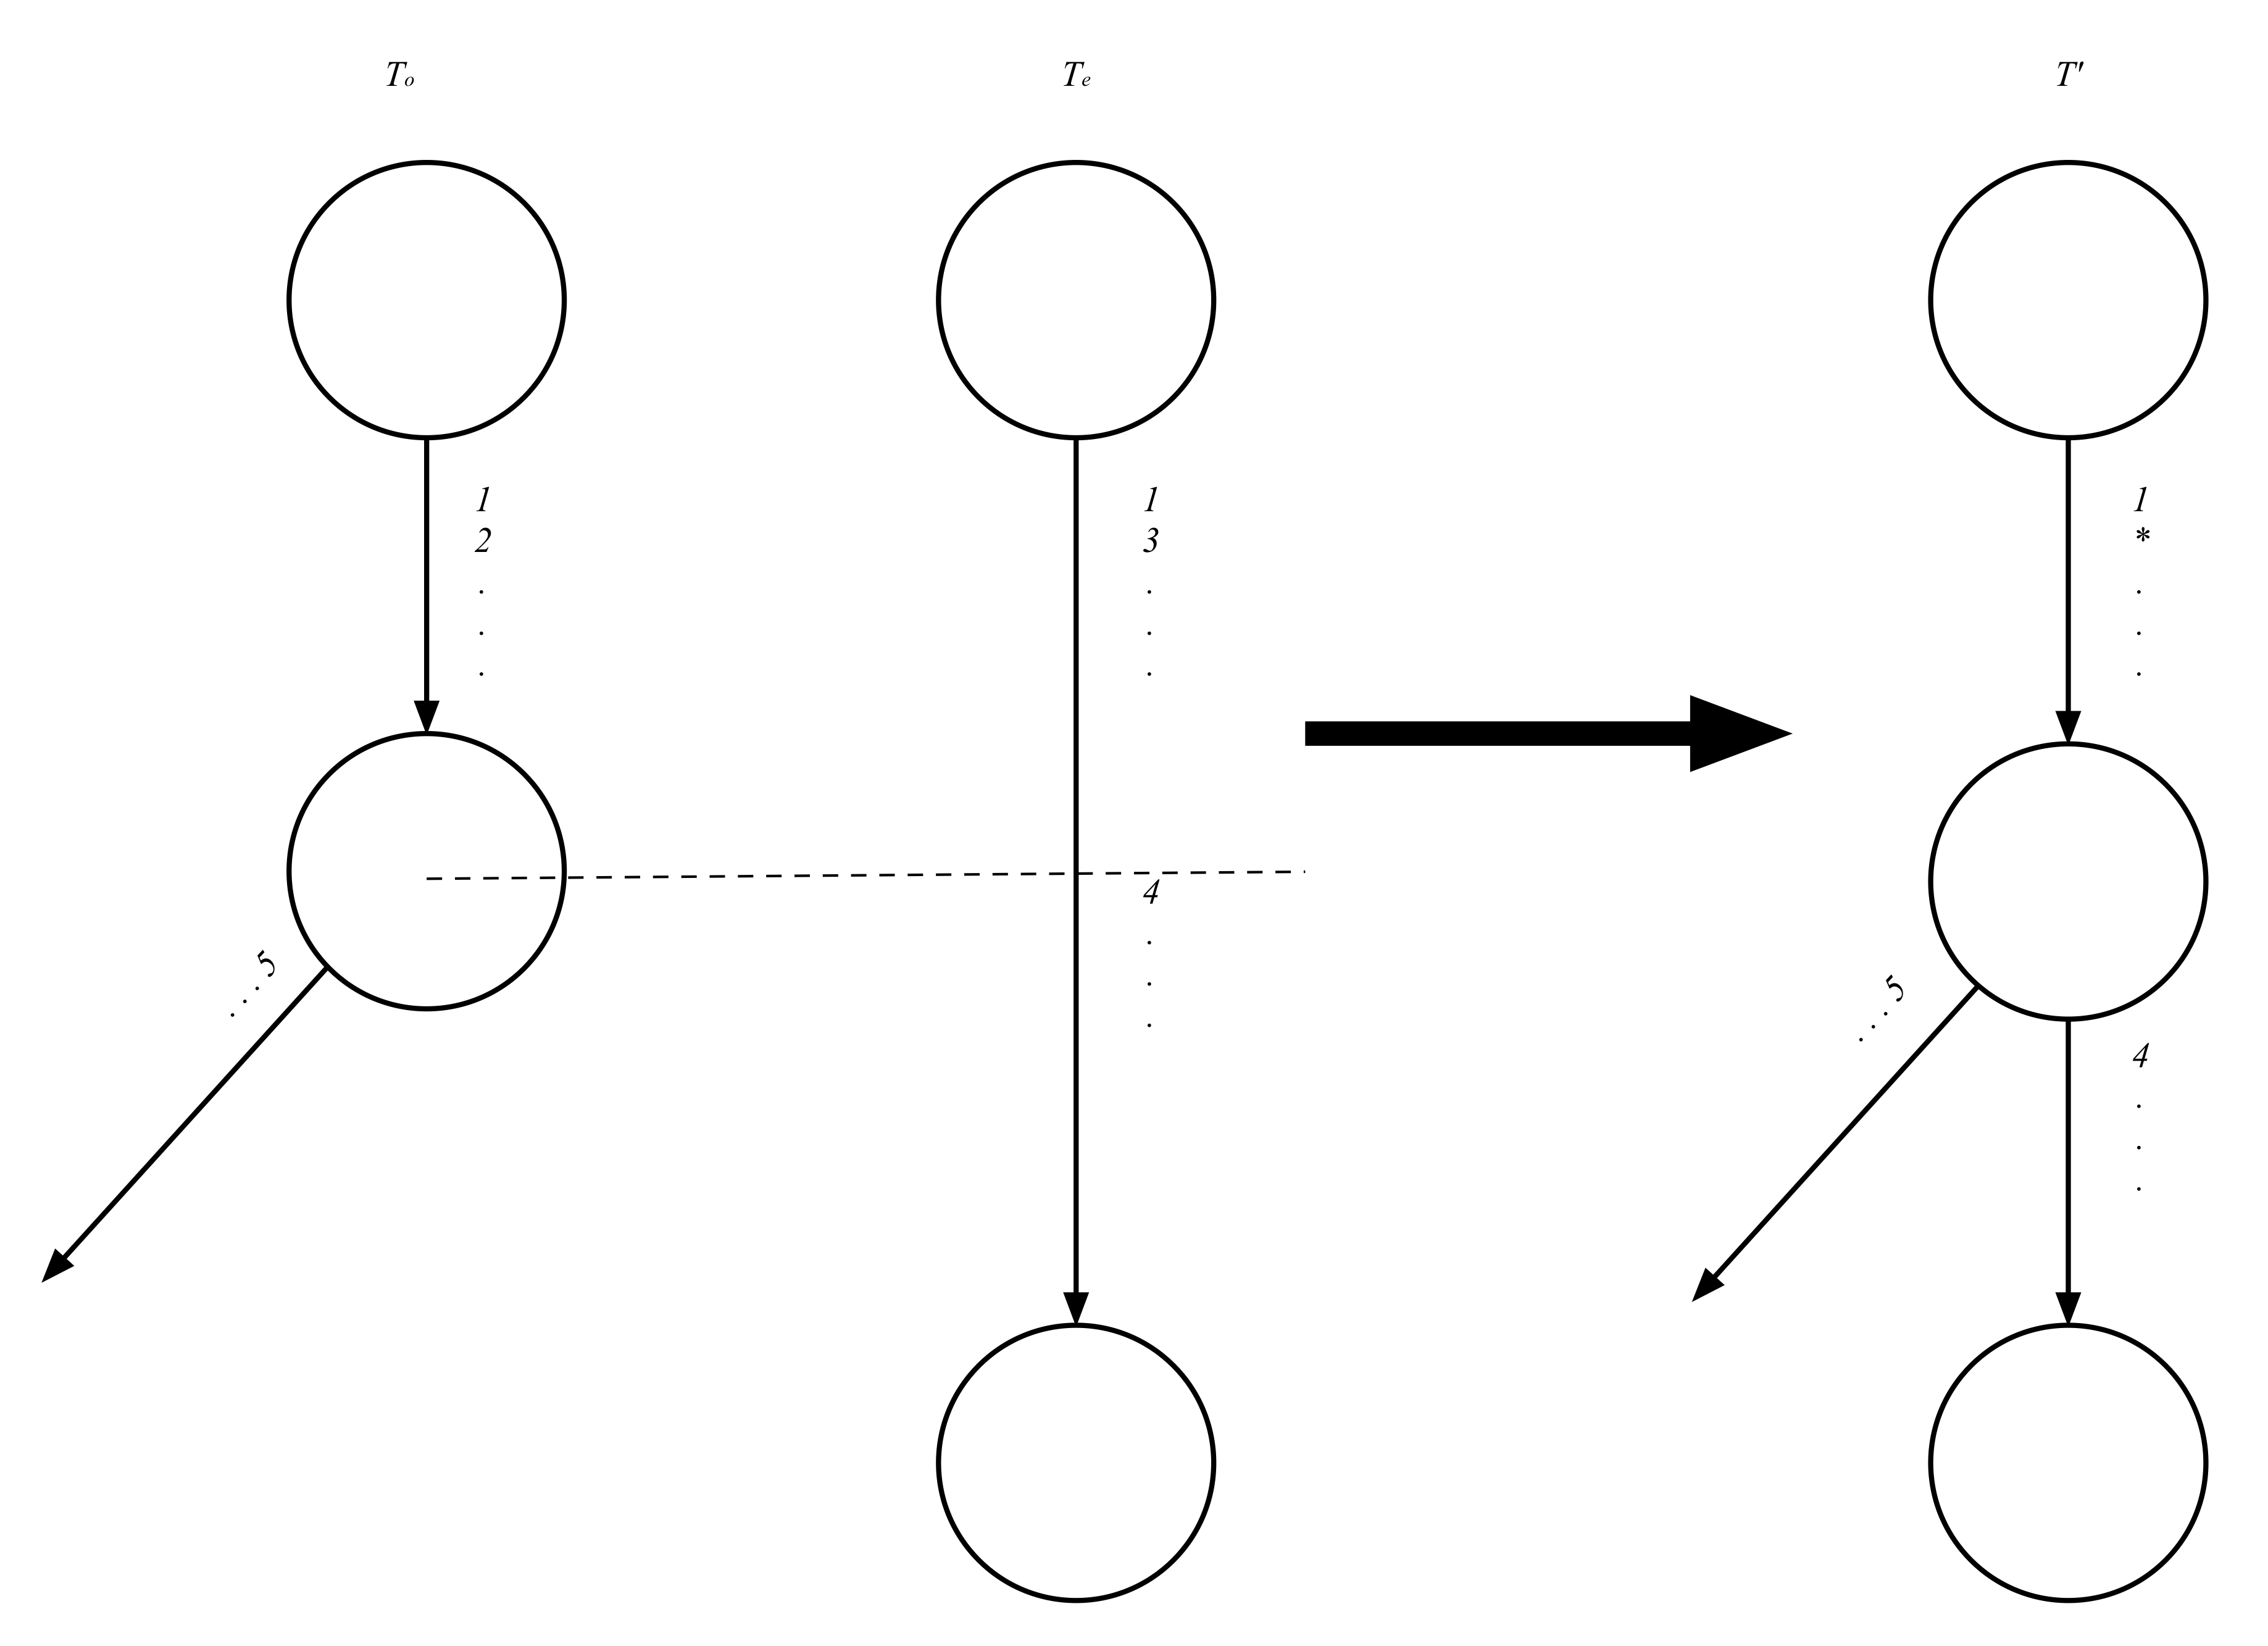
\includegraphics[scale=0.1,keepaspectratio=true]{graphics/farach-suffix-tree-overmerging.jpg}
 % overmergingSuffixTrees.jpg: 3674x2666 px, 72dpi, 129.61x94.05 cm, bb=0 0 3674 2666
\end{center}


Wiedząc jak jest konstruowane drzewo $T'$, zapiszmy kroki do stworzenia poprawnego drzewa $T$:
\begin{enumerate}
 \item Stwórz $T'$ tak jak zostało to wyżej opisane.
 \item Wierzchołek drzewa $T'$, który ma odpowiadający wierzchołek w $T_o$ nazwijmy \textit{nieparzystym}, a jeśli ma odpowiadający wierzchołek w $T_e$, to nazwijmy go \textit{parzystym}. Pewne wierzchołki (np. korzeń) mogą być zarówno parzyste jak i nieparzyste.\\
 Teraz, dla każdego wierzchołka $u \in T'$ znajdź parę wierzchołków (jeśli istnieje) $(a,b)$, które są jego potomkami i liśćmi drzewa, a ponadto $a$ jest parzysty, $b$ jest nieparzysty oraz \verb|lca(a,b) = u|. Załóżmy, że \verb|word(a) = w[2i,n], word(b) = w[2j-1,n]|. Dodatkowo, każdemu liściowi $c$ takiemu, że \verb|word(c) = w[k,n]| nadajmy etykietę $l_k$. Zgodnie z tą konwencją $a = l_{2i}, \, b = l_{2j - 1}$.
 \\
 Zdefiniujmy funkcję $d$ taką, że $d(u) = lca(l_{2i+1}, l_{2j})$ i policzmy ją dla każdego $u$. Zauważmy, że jeśli $T'$ byłoby poprawnym drzewem, to $d(u) = suffix
\_link(u)$.
 \item Zakładając, że funkcja $d$ definiuje drzewo, dla każdego wierzchołka $u$ policz głębokość $L(u)$ w tym drzewie. Skorzystaj z faktu, że $lcp(w[2i,n], w[2j-1]) = L(lca(l_{2i}, l_{2j-1}))$ i stwórz tablicę $LCP_T$. 
\end{enumerate}
\subsection{Dowód poprawności}
Wystarczy udowodnić poprawność punktów $2.$ i $3.$
\begin{theorem}{}{}
Najdłuższy wspólny prefiks dowolnej pary liści $(a,b)$, takich, że $a$ - parzysty, $b$ - nieparzysty, i takich, że \verb|lca|$(a,b) = u$, jest taki sam.
\end{theorem}
\begin{proof}[Dowód]
Weźmy wierzchołek parzysty $u$ mający zarówno parzystego jak i nieparzystego potomka. Weźmy teraz dwóch parzystych potomków (być może takich samych) $u$: $l_{2i},\,l_{2j}$. Wówczas, \verb|lcp|$(w[2i,n],w[2j,n]) \geq |word(u)|$, ponieważ $u$, $l_{2i}$, $l_{2j}$ były w drzewie $T_e$.


Teraz, weźmy parę $l_{2i'-1}$, $l_{2j'-1}$ potomków $u$. Zachodzi wtedy \verb|lcp|$(w[2i'-1,n],w[2j'-1,n]) \geq |word(u)|$. Jest tak, ponieważ, jeśli $u$ był również w $T_o$, to działa ten sam argument co poprzednio. Jeśli nie był w $T_o$, to ponieważ $l_{2i'-1}$, $l_{2j'-1}$ są liśćmi, to musi istnieć wierzchołek $u' = $\verb| lca|$(l_{2i'-1}, l_{2j'-1}) \in T_o$, który jest potomkiem $u$ w $T'$. 


Rozważmy teraz parę liści $l_{2i''}$ i $l_{2j''-1}$ w $T'$, takich że $u = $\verb| lca|$(l_{2i''}, l_{2j''-1})$. Zachodzi wtedy \verb|lcp|$(w[2i'',n], w[2j''-1, n]) \leq |word(u)|$. Wynika to z faktu, że jeśli byłoby inaczej, to wtedy więcej niż jedna krawędź wychodząca z $u$ zaczynała by się tym samym znakiem, co jednak w $T'$ nie ma miejsca. Analogiczne rozumowanie możemy przeprowaddzić dla $u$ będącego wierzchołkiem nieparzystym i wówczas każda z powyższych nierówności również będzie zachodziła.

Weźmy w końcu liście $l_{2i'},$, $l_{2i''}$, $l_{2j'-1}$, $l_{2j''-1}$ takie, że \verb|lca|$(l_{2i'}, l_{2j'-1}) = $ \verb| lca|$(l_{2i''}, l_{2j''-1}) = u$. Wtedy, \verb|lcp|$(w[2i',n], w[2j'-1,n]) = k \leq |word(u)|$, co udowodniliśmy przed chwilą. Wiemy jednak, że \verb|lcp|$(w[2i',n], w[2i'',n]) \geq |word(u)| \geq k$, a zatem musi zachodzić także \verb|lcp|$(w[2i'' \ldots n], w[2j'-1 \ldots n]) = k$. Podobnie, \verb|lcp|$(w[2i'' \ldots n], w[2j''-1 \ldots n]) = k$. Wobec tego:
\begin{align*}
    lcp(w[2i',n],w[2j'-1,n]) = lcp(w[2i'',n], w[2j''-1,n]) = k.
\end{align*}
\end{proof}

\begin{theorem}{}{}
Funkcja $d$ definiuje drzewo na wierzchołkach $T'$, a ponadto dla dowolnych $l_{2i}$ i $l_{2j-1}$ zachodzi $L($\verb|lca|$(l_{2i}, l_{2j-1})) = $\verb| lcp|$(w[2i,n], w[2j-1,n])$.
\end{theorem}
\begin{proof}[Dowód]
Dowód jest indukcyjny ze względu na długość \verb|lcp|. Jeśli \verb|lcp|$word[2i, n], word[2j-1,n]) = 0$, to wówczas $word[2i, n]$ i $word[2j-1,n]$ różnią się na pierwszym znaku, więc \verb|lca|$(l_{2i}, l_{2j-1}) = $\verb| root|, co wynika ze sposobu konstruowania drzewa $T'$.

Załóżmy teraz, że twierdzenie zachodzi dla pary sufiksów parzystych i nieparzystych, takich, że ich \verb|lcp| $< k$. Niech $l_{2i},\,l_{2j-1}$ będą liśćmi takimi, że \verb|lca|$(w[2i,n], w[2j-1,n]) = k > 0$. Ponadto, niech $u = $\verb| lca|$(l_{2i}, l_{2j-1})$. Wtedy $u$ nie jest korzeniem, bo $k > 0$.

Niech teraz $l_{2i'}$, $l_{2j'-1}$ będą liśćmi użytymi do zdefiniowania $d(u)$. Zatem, z definicji, $d(u) = $\verb| lca|$(l_{2i'+1},l_{2j'})$.

Z założeń indukcyjnych wiemy, że funkcja $d$ definiuje drzewo na dotychczas rozważonych wierzchołkach, a ponadto, że funkcja $L$ jest zdefiniowana na tych wierzchołkach i że zwraca poprawne wartości \verb|lcp|. Zatem, z faktu, że funkcja $d$ definiuje drzewo, wiemy że $L(u) = 1 + L(d(u))$. Ponadto, z faktu, że funkcja $L$ zwraca poprawne wartości dla dotychczas rozważonych wierzchołków wiemy, że $1 + L(d(u)) = 1 + $\verb| lcp|$(w[2i'+1,n],w[2j',n])$. Teraz, ponieważ $k > 0$ (w szczególności oznacza to, że $w[2i'] = w[2j'-1]$), zachodzi $1 + $\verb| lcp|$(w[2i'+1,n],w[2j',n]) = $\verb| lcp|$(w[2i',n],w[2j'-1,n])$. A z poprzedniego twierdzenia wiemy, że \verb|lcp|$(w[2i',n],w[2j'-1,n]) = $\verb| lcp|$(w[2i,n],w[2j-1,n])$.

Wobec tego, $L(u) = $\verb| lcp|$(w[2i,n],w[2j-1,n])$, a ponadto struktura zdefiniowana przez funkcję $d$ jest drzewem.
\end{proof}

\subsection{Złożoność}
\subsubsection{Tworzenie $T_o$}
\begin{enumerate}
\item Sortowanie pozycyjne dla par, w których maksymalna liczba jest mniejsza lub równa $n$ (tak jest, bo początkowe słowo spełnia to założenie, a każde następne powstaje przez zastąpienie elementu przez jego rangę) zajmuje $O(n)$ czasu.
\item Jeśli wszystkie inne kroki będą liniowe, to ten krok zajmie $T(n) = T(\frac{n}{2}) + O(n) = O(n)$ czasu.
\item Każdy element tablicy $A_{T_o}$ liczymy w czasie stałym, więc ten krok zajmuje $O(n)$ czasu.
\item Podobnie jak w poprzednim punkcie, mamy stały czas na przetworzenie jednego elementu tablicy, więc całość robimy w $O(n)$.
\item Jest możliwe skonstruowanie drzewa sufiksowego w czasie liniowym z tablic $A$ i $LCP$.\\ Idea: wstawiamy kolejne sufiksy w kolejności leksykograficznej. \\
Po wstawieniu każdego sufiksu, zatrzymujemy się w liściu, który go reprezentuje i dopóki \verb|lcp|$(word(v), next\_suffix) < |word(v)|$ wykonujemy, $v = v.parent$, a następnie dodajemy nową krawędź z wierzchołka $v$ albo dzielimy już wychodzącą.
\end{enumerate}
\subsubsection{Tworzenie $T_e$}
\begin{enumerate}
\item Da się w czasie liniowym zrobić preprocessing drzewa tak aby w czasie stałym odpowiadać na zapytania \verb|lca|. Jest to nietrywialny algorytm, który jest opisany w \url{https://www.ics.uci.edu/~eppstein/261/BenFar-LCA-00.pdf}.
\item Sortowanie pozycyjne na liczbach nieprzekraczających $n$ działą w $O(n)$.
\item Ponieważ zapytania o \verb|lcp| przetwarzane są w czasie stałym, czas działania tego kroku to $O(n)$.
\item Analogicznie jak dla $T_o$ - $O(n)$.
\end{enumerate}
\subsubsection{Łączenie drzew $T_o$ i $T_e$}
\begin{enumerate}
\item Ten krok to zwykły DFS działający liniowo względem sumarycznej ilości wierzchołków w drzewach $T_o$ i $T_e$, a ponieważ są to poprawne drzewa sufiksowe, to mają liniowe rozmiary względem $O(\frac{n}{2})$.
\item Odpowiednią parę liści dla każdego wierzchołka z $T'$ możemy znaleźć przy pomocy jednego DFS-a, korzystając z obliczonych wcześniej wartości dla potomków tego wierzchołka.

Funkcję $d$ liczymy dla każdego wierzchołka w czasie stałym, po wcześniejszym liniowym przetworzeniu drzewa $T'$ do zapytań o \verb|lca|.
\item Głębokość w drzewie liczymy ponownie używając algorytmu DFS i korzystając z obliczonych wartości, każdy element $LCP_T$ liczymy w czasie stałym. Odtworzenie drzewa z tablic $A_T$ i $LCP_T$ wykonujemy w czasie $O(n)$, jak wyżej.
\end{enumerate}

\subsubsection{Algorytm Karpa-Millera-Rosenberga}

Algorytm \emph{prefix-doubling}, zaproponowany w \citep{karp1972rapid}, opiera się na pomyśle prostej rekurencji. Załóżmy, że dla podsłów $t[i:i + k]$\footnote{Ściślej chodzi nam o $t[i:\min \{i + k, n\}]$ -- albo można równoważnie założyć, że na końcu dodajemy nieskończony ciąg symboli $\$$.} dla pewnego $k \ge 1$ oraz $1 \le i \le n$ mamy dostęp do funkcji $rank(i, k)$, zwracającej numer $t[i:i + k]$ w porządku leksykograficznym.
Wówczas wystarczy umieć wyznaczać na jej podstawie efektywnie wartości $rank(i, 2k)$ dla wszystkich $1 \le i \le n$.

\begin{code}
\captionof{listing}{Algorytm Karpa-Millera-Rosenberga budowania tablicy sufiksowej}
\inputminted{python}{code/suffix-array/kmr.py}
\label{alg:suffix-array-kmr}
\end{code}

\begin{lemma}{crochemore2007algorithms}{Lemma 4.8, s. 169-170}
  Dla dowolnych $1 \le i \le n$ oraz $k \ge 1$ wartość $rank(i, 2k)$ jest równa pozycji pary $(rank(i, k), rank(i + k, k))$ w porządku leksykograficznym na wszystkich takich parach.
\end{lemma}

\begin{proof}
  Z założenia, $rank(i, k) < rank(j, k)$ wtedy i tylko wtedy, gdy $t[i: i + k] < t[j: j + k]$ oraz $rank(i, k) = rank(j, k)$ wtedy i tylko wtedy, gdy $t[i: i + k] = t[j: j + k]$ dla dowolnych $i$, $j$, $k$.

  Jeśli $t[i: i + k] < t[j: j + k]$, to oczywiście zachodzi $t[i: i + 2 k] < t[j: j + 2 k]$ dla dowolnych $i$, $j$, $k$.
  Podobnie jeśli $t[i: i + k] = t[j: j + k]$ oraz $t[i + k + 1: i + 2 k] = t[j + k + 1: j + 2 k]$, to również $t[i: i + 2 k]$ < $t[j: j + 2 k]$ dla dowolnych $i$, $j$, $k$.

  Składając te wszystkie obserwacje razem, otrzymujemy wprost, że $t[i: i + 2 k]$ < $t[j: j + 2 k]$ wtedy i tylko wtedy, gdy $rank(i, 2 k) < rank(j, 2 k)$ dla dowolnych $i$, $j$, $k$.

  Aby zakończyć dowód wystarczy zaobserwować, że dla dwóch sąsiednich elementów w porządku $rank(i, 2 k)$ nie może również istnieć żaden element rozdzielający je w porządku par $(rank(i, k), rank(i + k, k))$.
\end{proof}

\begin{corollary}{}{}
  Algorytm \ref{alg:suffix-array-kmr} zwraca poprawną tablicę sufiksową.
\end{corollary}

\begin{proof}
  Po $\log{n}$ iteracjach głównej pętli otrzymujemy z $rank(i, 1)$ tablicę wartości $rank(i, n)$ -- a to z definicji jest dokładnie tablica sufiksowa.
\end{proof}

\begin{theorem}{}{}
  Algorytm \ref{alg:suffix-array-kmr} wykonuje się w czasie $O(n \log{n})$.
\end{theorem}

\begin{proof}
  Całkowita złożoność algorytmu \ref{alg:suffix-array-kmr} zależy od zastosowanego sortowania.
  Jeśli jest to sortowanie pozycyjne (\emph{radix sort}), to pojedyncza iteracja wymaga czasu $O(n)$. Iteracji mamy dokładnie $\log{n}$.
\end{proof}

\subsubsection{Algorytm K\"arkk\"ainena-Sandersa}

Algorytm \emph{skew}, wprowadzony w \citep{karkkainen2003simple}, umożliwia zejście do liniowego czasu obliczania tablicy sufiksowej.
Wymaga on założenia o tym, że alfabet można utożsamić ze zbiorem liczb naturalnych. W przeciwieństwie jednak np. do problemu sortowania w algorytmach tekstowych jest to założenie bardzo naturalne i często spotykane w praktyce (podobnie jak założenie, że $|\A| = O(1)$).

Sednem algorytmu K\"arkk\"ainena-Sandersa jest zamiana słowa $t$ na słowo $t'$ takie, że $|t'| = \frac{2}{3} |t|$.
Zauważmy, że bez straty ogólności możemy założyć, że słowo $t$ jest długości podzielnej przez $3$ -- wystarczy dołożyć na koniec odpowiednią liczbę znaków $\# \notin \A$ takich, że $\# > a$ dla każdego $a \in \A$.

Dokładniej, niech $triple(i)$ oznacza pozycję $t[i:i+3]$ wśród wszystkich unikalnych trzyliterowych podsłów $t$ posortowanych leksykograficznie.
Tworzymy nowe słowo $t'$ w następujący sposób:
\begin{align*}
  t' = triple(1) \cdot triple(4) \ldots \cdot triple(2) \cdot triple(5) \ldots
\end{align*}
Zwrócony wynik dla tego słowa umożliwia odrębne posortowanie sufiksów $t$ osobno dla zbiorów
\begin{align*}
  P_{12} & = \left\{1 \le i \le n: i \mod 3 \in \{1, 2\}\right\} \\
  P_0 & = \left\{1 \le i \le n: i \mod 3 = 0\right\}.
\end{align*}
Co więcej, na podstawie danego $t'$ możliwe jest scalenie również częściowych tablic sufiksowych dla $P_{12}$ i $P_0$.

\begin{code}
\captionof{listing}{Algorytm K\"arkk\"ainena-Sandersa budowania tablicy sufiksowej}
\inputminted{python}{code/suffix-array/skew.py}
\label{alg:suffix-array-skew}
\end{code}

\begin{problem}{}{}
  Pokaż że \ref{alg:suffix-array-skew} na podstawie $t'$ wyznacza poprawnie tablicę sufiksów dla $P_{12}$.
\end{problem}

\begin{problem}{}{}
  Pokaż że \ref{alg:suffix-array-skew} na podstawie $t'$ wyznacza poprawnie tablicę sufiksów dla $P_0$.
\end{problem}

\begin{theorem}{}{}
  Algorytm \ref{alg:suffix-array-skew} na podstawie $t'$ poprawnie scala tablice sufiksów dla $P_{12}$ i $P_0$.
\end{theorem}

\begin{proof}
  Na mocy założenia mamy dostępne posortowane listy sufiksów osobno dla indeksów należących do $P_{12}$ i $P_0$.
  
  Scalenie odbywa się zgodnie z funkcją \emph{merge} identyczną jak w algorytmie mergesort. Mamy 2 przypadki:
  \begin{enumerate}
    \item jeśli mamy $i \in P_{12}$ takie, że $i \mod 3 = 2$ oraz pewne $j \in P_0$, to wiemy, że $i + 1, j + 1 \in P_{12}$ -- wystarczy zatem porównać ze sobą pary $(t[i], S[i + 1])$ i $(t[j], S[j + 1])$,
    \item jeśli mamy $i \in P_{12}$ takie, że $i \mod 3 = 1$ oraz pewne $j \in P_0$, to wiemy, że $i + 2, j + 2 \in P_{12}$ -- wówczas postępujemy podobnie, tylko porównujemy trójki $(t[i], t[i + 1], S[i + 2])$ i $(t[j], t[j + 1], S[j + 2])$.
  \end{enumerate}
  Zauważmy, że $S[i + 1]$, $S[i + 2]$ lub $t[i + 1]$ mogą nie istnieć (podobnie dla $j$). Wówczas wystarczy zwracać wartości, które będą zawsze mniejsze od wartości odpowiednio z $S$ lub $\A$.
\end{proof}

\begin{theorem}{}{}
  Czas działania algorytmu \ref{alg:suffix-array-skew} wynosi $O(n)$.
\end{theorem}

\subsubsection{Wykonywanie zapytań w czasie $O(m \log{n})$}

Sprawdzanie, czy słowo $w$ o długości $m$ występuje w tekście $t$ dla danej tablicy sufiksowej $SA(t)$ jest wykonalne w czasie $O(m \log{n})$: wystarczy zwykłe binarne wyszukiwanie słowa $w$ w $SA(t)$.

Co więcej, tablica sufiksowa umożliwia nie tylko zliczenie wszystkich wystąpień słowa $w$ w tekście w czasie $O(m \log{n})$, ale również odnalezienie ich w czasie $O(m \log{n} + k)$. Wystarczy tylko wyszukać pozycje odpowiadające słowom $w$ oraz $w\#$, gdzie $\# \notin \A$ oraz $a < \#$ dla każdego $a \in \A$. Pozycje te wyznaczają w tablicy $SA(t)$ sekwencję początków sufiksów, dla których $w$ musi być prefiksem -- chociaż niekoniecznie w kolejności rosnącej.

\subsubsection{Wykonywanie zapytań w czasie $O(m + \log{n})$}

\todo[inline]{Algorytm Manbera-Myersa}

\subsubsection{Dalsze zagadnienia}

\citet{li2018optimal} pokazali algorytm obliczania tablicy sufiksowej w czasie $O(n)$ wymagający zaledwie $O(1)$ dodatkowej pamięci.


\section{Algorytm small-large}


\subsection{Tablica sufiksów}
Dla słowa s niech $T_i$ oznacza sufiks rozpoczynający się na indeksie $i$, a $t_i$ to znak na $i$-tej pozycji. Tablica sufiksów słowa $s$ to tablica zawierająca indeksy sufiksów $s$ posortowanych według porządku leksykograficznego tych sufiksów. Tablica ta przydaje się np. przy budowaniu drzew sufiksowych. Poniżej przedstawiony jest algorytm budujący tablicę sufiksów w czasie i pamięci liniowej.

W poniższych rozważaniach bez straty ogólności zakładamy, że każde słowo $s$ kończy się znakiem unikalnym i najmniejszym w słowie. Zakładamy również że alfabet to $\{1,2,...,n\}$.

\subsection{SL - kategoryzacja sufiksów}

Na początek przedstawimy kategoryzacje prefiksów na typy S (small) i L (large). Główna idea algorytmu jest oparta właśnie na tej kategoryzacji i jej własnościach.

\begin{definition}{}{}
Sufiks $i$ jest typu S/L, gdy jest mniejszy/większy od sufiksu $i+1$. Sufiks $n$ jest S i L (zależnie od potrzeby).
\end{definition}

Można, używając poniższego faktu, w czasie i pamięci liniowej dokonać kategoryzacji sufiksów na typy S/L.

\begin{remark-thm}
Dla sufiksu $T_i \ (i<n)$:

\begin{itemize}
\item jeśli $t_i \neq t_{i+1}$, to wystarczy porównać jeden znak aby dowiedzieć się jakiego typu jest $T_i$
\item
jeśli $t_{i} = t_{i+1}$, to znajdź pierwszy $j > i$, taki że $t_j \neq t_i$, wtedy \\
$ t_j > t_i \Rightarrow T_i,T_{i+1},...,T_{j-1}$ są typu S \\
$ t_j < t_i \Rightarrow T_i,T_{i+1},...,T_{j-1}$ są typu L
\end{itemize}

\end{remark-thm}

Przedstawmy również ważną własność kategoryzacji SL.

\begin{lemma}{}{}
\label{SL_order}
Sufiks typu S jest leksykograficznie większy od każdego sufiksu typu L, który rozpoczyna się tym samym znakiem.
\end{lemma}
\begin{proof}
Dowód nie wprost - załóżmy że istnieją sufiksy: $T_i = c \alpha c_1 \beta$ typ S i $T_j = c\alpha c_2 \gamma$ typ L, $c, c_1, c_2 \in \Sigma$, $\alpha, \beta, \gamma \in \Sigma^*$, $c_1 \neq c_2$, takie że $T_i < T_j$.

\item[Case 1:] $\alpha$ zawiera znak inny niż $c$\\
Niech $c_3$ - znak $\neq c$ najbardziej na lewo w $\alpha$. $T_i$ jest typu S, więc $c_3>c$. Podobnie z $T_j$ typu L otrzymujemy $c_3<c$, sprzeczność.

\item[Case 2:] $\alpha$ zawiera tylko $c$ lub jest puste\\
Z typów $T_i$ i $T_j$ mamy $c_1 \geq c$ i $c \geq c_2$ (dowód podobnie jak case 1). Stąd $c_1 \geq c_2$, co daje sprzeczność z $T_i < T_j$.

\end{proof}

\subsection{Algorytm small-large}

Na algorytm można patrzeć w dwóch fazach - sortowanie sufiksów S/L, w zależności których z nich jest mniej. Następnie wykorzystujemy otrzymane informacje utworzenie porządku na wszystkich sufiksach. Wybieranie gałęzi z mniejszą ilością prefiksów danego typu jest konieczne aby zachować złożoność, ale nie wpływa na poprawność algorytmu.

\begin{algorithmic}
\Procedure{small-large}{s}%\Comment{compute suffix array}
\State $SL \gets$ \Call{SL-categorization}{$s$}
\State if $SL.count("S") < len(n)/2$
	\State $sortedS \gets$ \Call{sortS}{$s$, $SL$}
	\State \Return \Call{finishS}{$s$, $SL$, $sortedS$}
\State Else
	\State $sortedL \gets$ \Call{sortL}{$s$, $SL$}
	\State \Return \Call{finishL}{$s$, $SL$, $sortedS$}
\EndProcedure
\end{algorithmic}

W kolejnych sekcjach opisane zostaną bardziej szczegółowo funkcje $sortS$ i $finishS$. Procedury dla typu L są bardzo podobne - należy przeglądać niektóre listy w odwrotnej kolejności, operacje przeniesienia na początek/koniec grupy zamienić na przeniesienie na koniec/początek i zastąpić odniesienia do typu S odniesieniami do typu L.

\subsection{Sortowanie S sufiksów - faza 1}

\begin{definition}{}{}
S odległość - dystans od $i$ do najbliższego na lewo S sufiksu (nie wliczając $i$).
\end{definition}

\begin{definition}{}{}
S podsłowo - podsłowo $t[i,i+1,...,j]$, gdzie $i$ oraz $j$ to S sufiksy, a pomiędzy są same L sufiksy.
\end{definition}

\begin{definition}{}{}
Jeśli słowo $t[i,i+1,...,j]$ jest S podsłowem, to każdy jego prefiks nazywamy prefiksem S podsłowa.
\end{definition}

S podsłowa są ściśle powiązane z S sufiksami - gdy weźmiemy ciąg kolejnych S podsłów i skleimy je ze sobą, otrzymamy S sufiks modulo duplikaty znaków na zetknięciu podsłów.


\begin{algorithmic}
\Procedure{sortS}{s, SL}
\State $SsubstrPrefixes \gets$ S substring prefixes, divided by Sdist, bucketed and sorted by first character
\State $Ssubstr \gets$ S substrings, bucketed and sorted by first character
\State For $d \gets 1,...,max\_Sdist$
\State For $j$ in $SsubstrPrefixes[d]$
\State move $j-d$ to the front of its group in $Ssubstr$
\State EndFor
\State update groups in $Ssubstr$ using old $Ssubstr$ and $SsubstrPrefixes[d]$ 
\State EndFor
\State $s' \gets$ map $Ssubstr$ to its buckets number, ordered as in $s$
\State \Return unmap \Call{small-large}{$s'$}
\EndProcedure
\end{algorithmic}

Po pętli for S podsłowa są uporządkowane w kolejności prawie leksyko-graficznej. Jedyny wyjątek to gdy $\alpha$ jest podsłowem $\beta$, wtedy $\alpha > \beta$ w tym porządku.

Oznaczmy jako $T'_i$ sufiks w $s'$ odpowiadający S sufiksowi $T_i$. Poprawność sortowania wynika z poniższego faktu.

\begin{lemma}{}{}
$T_i < T_j \iff T'_i < T'_j$
\end{lemma}
\begin{proof}
\item[$T_i < T_j \Rightarrow T'_i < T'_j$] - trywialnie z mapowania
\item[$T_i < T_j \Leftarrow T'_i < T'_j$] - opis idei\\
Rozważa się pierwszy znak różniący $T'_i < T'_j$. Jest to numer jakiejś grupy, która indukuje S podsłowo. Odzyskujemy te podsłowa $\alpha,\beta$ i rozważamy dwa przypadki - $\beta$ to prefiks $\alpha$ lub nie. Z tego można wywnioskować $T_i < T_j$.
\end{proof}


\subsection{Sortowanie całości - faza 2}


\begin{algorithmic}
\Procedure{finishS}{s, SL, sortedS}
\State $A \gets$ bucket and sort $s$ suffixes by first character
\State For $x$ in $reversed(sortedS)$ \Comment{\Cref{SL_order}}
\State move $x$ to the end of its bucket in $A$
\State move that buckets end to the left by one
\State EndFor
\State For $i \gets 1,...,n$ \Comment{\cref{phase2-invariant}}
\State If $SL[A[i]-1] == "L"$
\State move $A[i]-1$ to the front of its bucket
\State move that buckets front to the right by one
\State EndIf
\State EndFor
\State \Return A
\EndProcedure
\end{algorithmic}


Po pierwszej pętli sufiksy typu S są już na poprawnych pozycjach. Pętla druga porządkuje resztę.

\begin{lemma}{}{}\label{phase2-invariant}
W kroku i drugiej pętli algorytmu, sufiks $T_{A[i]}$ jest już na poprawnej pozycji w tablicy sufiksów.
\end{lemma}
\begin{proof}
Indukcja.
\item[Baza indukcji:] wynika z tego, że najmniejszy sufiks jest typu S wiec jest już na poprawnej pozycji
\item[Krok indukcyjny $i \rightarrow i+1$:] nie wprost - istnieje sufiks $k > i+1$, który w tablicy sufiksów powinien zająć miejsce $A[i+1]$.\\
Wprost z założenia $T_{A[k]} < T_{A[i+1]}$ i obydwa te sufiksy są typu L - sufiksy S są na poprawnych miejscach.\\
$T_{A[k]}$ i $T_{A[i+1]}$ muszą rozpoczynać się tą samą literą $c$ - przez wcześniejsze dzielenie na grupy przez pierwszą literę $T_{A[i+1]}$ ma jako pierwszą najmniejszą literę z sufiksów $A[i+1],A[i+2],...,A[n]$. Niech $T_{A[i+1]}=c \alpha$ i $T_{A[k]}=c \beta$.\\
\begin{gather*}
T_{A[k]}\ is\ type\ L \Rightarrow \beta < T_{A[k]}\\
T_{A[k]} < T_{A[i+1]} \Rightarrow \beta < \alpha\\
(T_{A[k]}\ is\ A[i+1]th\ in\ suffix\ array) \land \beta < T_{A[k]} \Rightarrow \beta \in \{A[1],A[2],...,A[i]\}
\end{gather*}
$\beta < \alpha$, więc $T_{A[k]}$ był przesunięty na początek grupy (w gałęzi if) przed $T_{A[i+1]}$. Sufiksy te należą do tej samej grupy, zatem $T_{A[k]}$ leży na lewo od $T_{A[i+1]}$, sprzeczność.
\end{proof}

Z \Cref{SL_order} i \Cref{phase2-invariant} wynika poprawność algorytmu.


\subsection{Złożoność}
Ze względu na rekurencję $T(n) = T(n/2) + \mathcal{O}(n)$ otrzymujemy złożoność czasową i pamięciową liniową w stosunku do długości słowa.


\subsection{Tablica największych wspólnych prefiksów}

\todo[inline]{Konstrukcja tablicy LCP.}

\begin{theorem}{}{}
  Algorytm Kasai zwraca poprawną tablicę sufiksową.
\end{theorem}

\begin{proof}{}{}
  Weźmy dwa dowolne sufiksy słowa $t$ sąsiednie w porządku leksykograficznym tj. zaczynające się na pozycjach $SA[i]$ oraz $SA[i + 1]$ dla pewnego $1 \le i \le n - 1$. Niech długość najdłuższego wspólnego prefiksu $LCP(t[SA[i]:n], t[SA[i + 1]:n]) = k$ dla pewnego $k \ge 0$.

  Weźmy teraz $j$ takie, że $SA[j] = SA[i] + 1$, tj. $t[SA[j]:n] = t[SA[i] + 1:n]$. Wówczas wiemy, że
  \begin{align*}
    LCP(t[SA[j]:n], t[SA[j + 1]:n]) \ge \max\{LCP(t[SA[i]:n], t[SA[i + 1]:n]) - 1, 0\},
  \end{align*}
  ponieważ $t[SA[j]:n] < t[SA[j + 1]:n] \le t[SA[i + 1] + 1:n]$
  oraz
  \begin{align*}
    LCP(t[SA[j]:n], t[SA[i + 1] + 1:n])
        & = LCP(t[SA[i] + 1:n], t[SA[i + 1] + 1:n]) \\
        & = \max\{LCP(t[SA[i]:n], t[SA[i + 1]:n]) - 1, 0\}.
  \end{align*}
  Wykorzystujemy tu prosty fakt, że jeśli mamy dowolne słowa $w_1 \le w_2 \le w_3$, to $LCP(w_1, w_2) \ge LCP(w_1, w_3)$.

  Jeśli nie istnieje szukane $j$, to $SA[i] = n$, a zatem rzecz jasna $t[SA[i] + 1:n] = \varepsilon$, a zatem jego najdłuższy wspólny prefiks z dowolnym innym podsłowem wynosi $k = 0$.
\end{proof}

\begin{theorem}{}{}
  Liczba różnych podsłów dla słowa $t$ ($|t| = n$) wynosi
  \begin{equation*}
    \binom{n}{2} - \sum_{i = 1}^{n - 1} LCP[i]
  \end{equation*}
\end{theorem}

\begin{proof}
  Wystarczy policzyć podsłowa zaczynające się na pozycjach $SA[i + 1]$ dla $0 \le i \le n - 1$ tj. prefiksy $t[SA[i + 1]:n]$ niebędące prefiksami słów $t[SA[j]:n]$ dla $1 \le j \le i$.
  
  Ponieważ sufiksy są posortowane, to wiemy, że każdy prefiks $t[SA[i + 1]:n]$ długości $0 \le k < LCP[i]$ już wystąpił wcześniej -- w szczególności jako prefiks $t[SA[i]:n]$.
  
  Dalej, wiemy że $t[SA[i]:n] < t[SA[i + 1]:SA[i + 1] + LCP[i] + 1]$, ponieważ słowa są posortowane oraz $t[SA[i + 1] + LCP[i] + 1]$ jest z definicji $LCP$ pierwszym znakiem różnym w słowach $t[SA[i]:n]$ i $t[SA[i + 1]:n]$. Oczywiście z przechodniości relacji $<$ wynika, że również
  \begin{align*}
    t[SA[j]:n] \le t[SA[i]:n] < t[SA[i + 1]:SA[i + 1] + LCP[i] + k]
  \end{align*}
  dla wszystkich $k \ge 1$ oraz $1 \le j \le i$, a zatem każdy prefiks $t[SA[i + 1]:n]$ długości większej niż $LCP[i]$ na pewno nie jest prefiksem $t[SA[j]:n]$ dla $1 \le j \le i$.
  
  $t[SA[i + 1]:n]$ ma łącznie $n - SA[i + 1]$ prefiksów, więc takich prefiksów jest oczywiście $n - SA[i + 1] - LCP[i]$. Dla $i = 0$ oczywiście będzie to tylko $n - SA[1]$.
  Ostatecznie, całkowita liczba różnych słów wynosi
  \begin{align*}
    \sum_{i = 0}^{n - 1} \left(n - SA[i + 1]\right) - \sum_{i = 1}^{n - 1} LCP[i - 1] = \binom{n}{2} - \sum_{i = 1}^{n - 1} LCP[i],
  \end{align*}
  ponieważ $\sum_{i = 0}^{n - 1} \left(n - SA[i + 1]\right)$ to zarazem liczba wszystkich (niekoniecznie różnych) podsłów w tekście.
\end{proof}

\subsection{Suffix trays}

\todo[inline]{Uzupełnić -- ale z niskim priorytetem}

\input{13-factorization.tex}
\section{Odległość edycyjna}

\begin{algorithm}[H]
    \caption{Odległość edycyjna}
    \Input{Słowa $t_1, t_2 \in \A^+$ ($|t_i| = n_i$ dla $i = 1, 2$)}
    \Output{Minimalna liczba operacji typu \emph{insert}, \emph{delete} i \emph{substitute} przeprowadzająca słowo $t_1$ w $t_2$.}
\end{algorithm}

Zwróćmy uwagę, że analogiczny problem, w którym dozwolona jest tylko operacja \emph{substitute} to obliczanie odległości Hamminga. Można ją wprost wyznaczyć przeglądając $t_1$ i $t_2$ od lewej do prawej, zliczając pozycje, dla których $t_1[i] \neq t_2[i]$.

\subsection{Algorytm Fischera-Wagnera}

Podstawowy algorytm obliczania odległości edycyjnej sprowadza się do sekwencyjnego obliczania wartości funkcji rekurencyjnej
\begin{align*}
  d_e(i, j) =
  \begin{cases}
    0 & \text{gdy $i = 0$ lub $j = 0$,} \\
    d_e(i - 1, j - 1) & \text{gdy $t_1[i] = t_2[j]$,} \\
    \min\{d_e(i - 1, j - 1), d_e(i - 1, j), d_e(i - 1, j - 1)\} + 1 & \text{gdy $t_1[i] \neq t_2[j]$.}
  \end{cases}
\end{align*}
Poprawność algorytmu wynika z indukcji ze względu na porządek par $(i, j)$. Czas działania algorytmu to $O(n_1 n_2)$.
Jak widać z powyższego wzoru, do obliczeń wystarczy zapamiętanie poprzedniego wiersza lub kolumny, więc wymagana pamięć wynosi $O(\min\{n_1, n_2\})$.

\begin{code}
\captionof{listing}{Obliczanie odległości edycyjnej w czasie $O(n_1 n_2)$ i pamięci $O(\min\{n_1, n_2\})$}
\inputminted{python}{code/other/edit-distance.py}
\label{alg:edit-distance}
\end{code}

Technika może być łatwo uogólniona do dowolnych macierzy ocen, przypisujących różne wagi za odległości dla operacji \emph{insert}, \emph{delete} i \emph{substitute}. Przykładem takiego wykorzystania są rodziny macierzy PAM i BLOSUM dla algorytmów dopasowań ciągów w zastosowaniach bioinformatycznych.

Można również łatwo zamienić problem na obliczanie funkcji podobieństwa jako maksymalnej (zamiast minimalnej) wartości dla danej macierzy operacji, tym razem interpretowanej jako macierz nagród \citep{sellers1974theory}.

\subsection{Technika czterech Rosjan}

Dla obliczeń macierzowych istnieje ogólna technika przyspieszania obliczeń, nazywana \emph{Four Russians speedup}\footnote{Najbardziej znanym z autorów był Jefim Dinic, znany również z algorytmu dla znajdowania maksymalnego przepływu w grafach.}.

Główna idea tej metody polega na podziale wejścia na małe bloki o niewielkim zakresie wartości.
Załóżmy, że pewien problem jest w ogólności rozwiązywany przez funkcję $y_n = f(y_{n - 1}, x_n)$, a jedna iteracja wymaga czasu $F(n)$ -- więc całość wykonuje się w czasie $\sum_{i = 1}^{n - 1} F(i)$.

Załóżmy teraz, że każda pozycja wejściowa pochodzi z małego zbioru $X$, a każda pozycja wyjściowa również z małego zbioru $Y$.
Wówczas dla dowolnego $k$ zawsze możemy obliczyć z wyprzedzeniem tablicę wszystkich $|X|^k |Y|$ wartości funkcji $f^{(k)}$, czyli $k$-krotnego złożenia $f$.
Wówczas można policzyć $f_n$ wykorzystując $\frac{n}{k}$ wyszukiwania w tablicy. Całkowity czas działania (zakładając stały dostęp do tablicy wartości) wynosi zatem
\begin{align*}
  |X|^k |Y| \sum_{i = 1}^{k - 1} F(i) + \frac{n}{k}.
\end{align*}
Przykładowo dla $F(n) = n^2$, $|X| = O(1)$ i $|Y| = O(n)$ wystarczy dobrać $k = \log_{|X|}{n}$, aby zmniejszyć czas wykonania z $O(n^3)$ do $O(n^2 \log^3{n})$.

Metoda ta używana jest m.in. do mnożenia i odwracania macierzy binarnych, a także do efektywnego liczenia domknięcia przechodniego grafu. Można ją również wykorzystać do optymalizacji algorytmu obliczającego odległość edycyjną \citep{masek1980faster}. Technika ta również uogólnia się na różnorodne macierze nagród i kar.

\paragraph{Omówienie algorytmu}

Odległość edycyjna pomiędzy dwoma słowami o długościach $n$ i $m$ jest definiowana jako minimalny koszt sekwencji operacji edytujących (dodania znaku, usunięcia znaku, zamiany jednego znaku w inny), które prowadzą do transformacji jednego słowa w drugie. Szczególnym przypadkiem problemu znajdywania odległości edycyjnej jest szukanie najdłuższego wspólnego podciągu dwóch słów. Rozwiązanie tego podproblemu w czasie szybszym niż $O(n^{2-\epsilon})$ (gdy słowa mają tę samą długość $n$), prowadziłoby do obalenia SETH. Autorzy pracy pokazują algorytm na szukanie odległości edycyjnej dwóch słów działający w czasie $O(n \cdot max(1,m/log n))$ pod warunkiem, że koszty operacji edycyjnych są całkowitymi wielokrotnościami tej samej liczby rzeczywistej, a alfabet jest skończony.

\paragraph{Przyjęte oznaczenia}

$A_n$ - n-ty znak słowa $A$\\
$A^{i,j}$ - słowo $A_i...A_j$\\
$D_a$ - koszt usunięcia znaku a\\
$I_a$ - koszt wstawienia znaku a\\
$R_{a,b}$ - koszt zamiany znaku a na znak b\\
$\delta$ - odległość edycyjna, minimum po sumie kosztów wszystkich możliwych sekwencji edycyjnych,
$\delta_{i,j}$ - odległość edycyjna między słowami $A^{1,i}$ oraz $B^{1,j}$\\

\paragraph{Algorytm Wagnera i Fischera}

Algorytm opisany w pracy opiera się na pomyśle z innego algorytmu, autorstwa Wagnera i Fischera. Algorytm ten wyznacza odległość edycyjną dynamicznie, w czasie proporcjonalnym do iloczynu długości słów. Tworzy w tym celu pomocniczą macierz o rozmiarze $(|A|+1) \times (|B|+1)$, w której komórka (i,j) odpowiada kosztowi $\delta_{i,j}$. Poniższe twierdzenia prezentują sposób obliczania bazy i kolejnych komórek:\\

\textbf{Twierdzenie 1}\\\\
$\delta_{0,0} = 0$ $\forall i,j : 1 \leq i \leq |A|, 1 \leq j \leq |B|$\\
$\delta_{i,0} = \sum_{1 \leq r \leq i}D_{A_r}$ oraz
$\delta_{0,j} = \sum_{1 \leq r \leq j}I_{B_r}$\\

\textbf{Twierdzenie 2}\\\\
$\delta_{i, j} = min(\delta_{i-1,j-1}+R_{A_i,B_j}, \delta_{i-1,j}+D_{A_i}, \delta_{i,j-1}+I_{B_j})$

\paragraph{Przyspieszenie metodą czterech Rosjan}

Technika "czterech Rosjan" pochodzi z algorytmu obliczania przechodniego domknięcia grafu skierowanego poprzez podział macierzy sąsiedztwa na podmacierze o niewielkiej ilości wierszy. Okazuje się, że podobny pomysł można wykorzystać do asymptotycznego przyspieszenia powyższego algorytmu, właśnie dzięki podziałowi obliczenia na dużo mniejszych obliczeń.\\

Zauważmy, że podmacierz $(i,j,m)$ macierzy edycyjnej z algorytmu Wagnera-Fischera - zaczynająca się w komórce $(i+1, j+1)$ i mająca rozmiar $m \times m$ - jest zdeterminowana tylko i wyłącznie poprzez koszt $\delta(i,j)$ oraz wektory inicjalne $\delta(i,j+1)...\delta(i,j+m)$ oraz $\delta(i+1,j)...\delta(i+m,j)$. Obliczając wartość w komórce $(i,j)$ odwołujemy się bowiem tylko do trzech sąsiednich komórek $(i-1,j-1), (i-1,j), (i, j-1)$. Możemy więc wcześniej dla każdej możliwej podmacierzy $(i,j,m)$ obliczyć i zapamiętać jej wektory finalne: $\delta(i+m,j+1)...\delta(i+m,j+m)$ oraz $\delta(i+1,j+m)...\delta(i+m,j+m)$.\\

Aby tego dokonać, musimy być w stanie wyenumerować wszystkie możliwe macierze rozmiaru $m$. Zakładamy, że alfabet jest skończony, więc słów długości $m$ jest skończona ilość. Jednak generowanie wszystkich możliwych wektorów inicjalnych może zająć zbyt dużo czasu - wartości komórek mają tendencję do wzrostu wraz z rozszerzaniem się macierzy głównej. Kiedy jednak ograniczymy funkcję kosztu do przypisywania operacjom edycyjnym wyłącznie wielokrotności jakiejś liczby rzeczywistej, okaże się, że mamy tylko skończoną ilość różnic pomiędzy sąsiednimi komórkami w macierzy edycyjnej.\\\\
Będziemy więc operować na wektorach różnic (kroków) pomiędzy komórkami sąsiadującymi ze sobą w poziomie lub pionie. Prowadzi to do następującej modyfikacji twierdzenia 2:\\

\textbf{Twierdzenie 2b}\\\\
$\delta_{i, j} - \delta_{i-1, j} =$\\
$min(R_{A_i,B_j} - (\delta_{i-1,j} - \delta_{i-1,j-1}), D_{A_i}, I_{B_j} + (\delta_{i,j-1} - \delta_{i-1,j-1}) - (\delta_{i-1,j} - \delta_{i-1,j-1}))$\\\\
$\delta_{i, j} - \delta_{i, j-1} =$\\
$min(R_{A_i,B_j} - (\delta_{i,j-1} - \delta_{i-1,j-1}), D_{A_i} + (\delta_{i-1,j} - \delta_{i-1,j-1}) - (\delta_{i,j-1} - \delta_{i-1,j-1}), I_{B_j})$\\\\

Proponowany w pracy \textbf{Algorytm Y} wykonuje pierwszy krok - generuje wszystkie możliwe pary $C, D$ słów długości $m$ oraz wszystkie możliwe wektory inicjalne różnic:  $R$ - pomiędzy sąsiednimi wierszami (wertykalny) i $S$ - pomiędzy sąsiednimi kolumnami (horyzontalny). Następnie oblicza odpowiadające danej podmacierzy wektory finalne różnic - $R'$ oraz $S'$, wyliczając kolejne wektory $T$ (wertykalne) i $U$ (horyzontalne), zgodnie ze wzorem z twierdzenia 2b. Obliczenie i zaindeksowanie każej możliwej podmacierzy zajmuje $O(m^2log m)$ czasu.\\

Następnie \textbf{Algorytm Z} łączy ze sobą podwyniki wygenerowane przez Algorytm Y i oblicza rzeczywistą odległość edycyjną. W tym celu dynamicznie oblicza kolejne finalne wektory dla podmacierzy $(i,j,m)$ dla $i \in \{0,m,...|A|*(m-1)\}$ oraz $j \in \{0,m,...|B|*(m-1)\}$, wykorzystując fakt, że wektor finalny danej podmacierzy jest wektorem inicjalnym dla sąsiadującej (odpowiednio pionowym lub poziomym). Rzeczywista odległość edycyjna może być następnie uzyskana jako suma wartości komórek na dowolnej ścieżce od komórki początkowej do końcowej (dodając kolejne różnice, docierając do ostatniej komórki otrzymamy jej wartość). Czas działania tej części to $O(|A| \cdot |B| \cdot (m+log|A|)/m^2)$. Jeśli wybierzemy $m = \lfloor log_k|A| \rfloor$, całość (Algorytm Y i Z) działa w czasie $O(|A| \cdot |B|/m)$.

\paragraph{Najdłuższy wspólny podciąg}

Powyższego algorytmu można również użyć do obliczenia najdłuższego wspólnego podciągu (LCS). W tym celu jako funkcje kosztu wybieramy:
$D_a = I_a = 1$ oraz $R_{a,b} = 0$ jeśli a=b oraz $R_{a,b} = 2$ w przeciwnym wypadku. Najtańszą ścieżką edycyjną jest w takim przypadku usunięcie z jednego słowa znaków z nie-LCS i dodanie do drugiego słowa znaków z LCS. Do odtworzenia LCS można wykorzystać pomysł analogiczny do odtwarzania ze standardowego algorytmu (Wagnera-Fischera). Zaczynając od ostatniej komórki w macierzy, patrzymy skąd otrzymaliśmy daną wartość i cofamy się. Za każdym razem kiedy operacją, którą wykonywaliśmy jest zamiana, a znaki się zgadzają - mamy do czynienia z literą z LCS. W przypadku algorytmu prezentowanego w pracy nie mamy obliczonej całej macierzy, ale możemy odtworzyć z wektorów inicjalnych podmacierze różnic przecinane przez ścieżkę. Wybór znaków należących do LCS będzie taki sam jak w przypadku rzeczywistej macierzy kosztów.

\section{Najdłuższy wspólny podciąg}

\begin{algorithm}[H]
    \caption{Najdłuższy wspólny podciąg}
    \Input{Zbiór słów $T = \{t_1, t_2, ..., t_k\} \subseteq \A^+$ takich, że $|t_i| \le n$ dla $1 \le i \le k$.}
    \Output{Słowo $t$ będące najdłuższym podciągiem wszystkich słów z $T$.}
\end{algorithm}

Problem najdłuższego wspólnego podciągu jest powiązany z problemem odległości edycyjnej.
Dla $|T| = 2$ niech $d(t_1, t_2)$ oznacza odległość dla dopuszczalnych operacji \emph{insert} i \emph{delete}.
Wówczas zachodzi
\begin{align*}
    |t_1| + |t_2| = 2 |t| + d(t_1, t_2),
\end{align*}
wystarczy bowiem zauważyć, że $t_1$ w $t$ przeprowadzają wszystkie operacje \emph{delete} a $t$ w $t_2$ -- \emph{insert}.

\subsection{Algorytm Needlemana-Wunscha}

Podstawowy algorytm obliczania najdłuższego wspólnego podciągu dla dwóch słów jest prostym rozszerzeniem algorytmu \ref{alg:edit-distance}. Jedyna różnica polega na konieczności trzymania całej tablicy odległości.
Odtwarzanie wyniku następuje na podstawie przejścia po ścieżce od ostatniej wartości tj. $d(t_1, t_2)$ do początku, odpowiadającemu $d(\epsilon, \epsilon)$.
Wybieramy rzecz jasna tylko te przejścia, które spełniają relację $\min$ w równaniu rekurencyjnym.

Oczywiście można odtwarzać kolejne przejścia i uzgodnione litery na podstawie $t_1$, $t_2$ porównując odpowiednie wartości macierzy $d$ -- lub też można zapisywać odpowiednie informacje równolegle w trakcie wypełniania tablicy $d$.

\begin{code}
\captionof{listing}{Obliczanie najdłuższego wspólnego podsłowa w czasie i pamięci $O(n_1 n_2)$}
\inputminted{python}{code/approximate-string-matching/needleman-wunsch.py}
\label{alg:lcs-needleman-wunsch}
\end{code}

\subsection{Algorytm Hirschberga}

Ponieważ dla dostatecznie dużych $n_1$ i $n_2$ w praktyce pamięć jest bardziej dotkliwą barierą niż czas, można zastanowić się nad usprawnieniem algorytmu, aby wykorzystywał tylko $O(\min\{n_1, n_2\})$ pamięci.

Okazuje się, że wystarczy zastosować podejście dziel-i-rządź. Z jednej strony jasne jest, że odpowiadająca najdłuższemu podciągowi optymalna ścieżka od punktu $(0, 0)$ do $(n_1, n_2)$ w macierzy $d$ musi przejść przez pewien punkt $(i, j)$ dla dowolnego $0 \le i \le n_1$. Możemy zatem wybrać $i$ w połowie aktualnie rozpatrywanego przedziału.

Znalezienie $j$ nie jest trudne. Okazuje się, że wystarczy do tego obserwacja z poniższego lematu:
\begin{problem}{}{}
  Punkt $(i, j)$ leży na (pewnej) optymalnej ścieżce w macierzy $d$ wtedy i tylko wtedy, gdy
  \begin{align*}
      j = \arg\max \{0 \le k \le n_2: d(t_1[1..i], t_2[1..k]) + d(\bar{t_1[i..n_2]}, \bar{t_2[k..n_2]})\}.
  \end{align*}
\end{problem}

\begin{code}
\captionof{listing}{Obliczanie najdłuższego wspólnego podsłowa w czasie $O(n_1 n_2)$ i pamięci $O(\min\{n_1, n_2\})$}
\inputminted{python}{code/approximate-string-matching/hirschberg.py}
\label{alg:lcs-hirschberg}
\end{code}

\subsection{Algorytm Myersa}

Algorytm omówiony w pracy służy do poszukiwania najdłuższego wspólnego podciągu. Powstał w oparciu o pracę \textbf{An O(ND) Diffrence Algorithm and Its Variations} autorstwa \textbf{Eugene'a W.Myers}.
\paragraph{Definicje}
Zanim przejdziemy do algorytmu zdefiniujmy graf edycji, definicje wspólnego podciągu oraz pewne pomocnicze określenia.

\paragraph{Graf edycji}
 Mając dane słowa $A = a_{1}a_{2}\dots a_{N}$ oraz $B = b_{1}b_{2}\dots b_{M}$ jako graf edycji G oznaczamy skierowany graf, dla którego zbiór wierzchołków to punkty siatki $(x,y),\:x\in[0,N]\:i\:y\in[0,M]$, natomiast na krawędzi składają się:
\begin{itemize}
    \item $(x-1,y) \xrightarrow{}(x,y)$ dla każdego $x\in[1,N]$ oraz $y\in[0,M]$.
    \item $(x,y-1) \xrightarrow{}(x,y)$ dla każdego $x\in[0,N]$ oraz $y\in[1,M]$.
    \item $(x-1,y-1) \xrightarrow{}(x,y)$ jeśli $a_{x} = b_{y}$, taka krawędź definiuje pewne dopasowanie pomiędzy wzorcami, punkty dla których $a_{x} = b_{y}$ nazwiemy punktami dopasowania.
\end{itemize}

\begin{definition}{}{Podciąg słowa}

Podciąg słowa A to każde słowo powstałe poprzez usunięcie 0 lub więcej symboli z A. Natomiast wspólny podciąg dwóch słów A i B to podciąg każdego z nich. 
\end{definition}

\paragraph{Graf edycji, a wspólny podciąg}

\begin{definition}{}{}
Śladem długości L nazywamy sekwencje L punktów dopasowania $(x_{1},y_{1}),(x_{2},y_{2})\dots(x_{L}, y_{L})$, gdzie dla każdego $1 \leq i < L:\:x_{i}<x_{i+1} \wedge y_{i}<y_{i+1}$. Jest to pewna sekwencji diagonalnych krawędzi. Ślad możemy powiązać z pewną ścieżka pomiędzy $(0,0)$ a $(N, M)$.
\end{definition}

Każdy ślad grafu edycji definiuje pewien wspólny podciąg słów A i B, który powstaje poprzez odpowiednie symbole zdefiniowane przez punkty dopasowania.

\begin{definition}{}{Odległość edycyjna}
Odległość edycyjna D to ilość operacji edycji które przeprowadzamy na tekście A żeby przeprowadzić go w tekst B. Jeśli spojrzymy na ścieżkę która zawiera pewien ślad L to każda krawędź pozioma w tej ścieżce definiuje pewną operację usunięcia symbolu z tekstu A, natomiast krawędzi pionowe definiują operację dodania symboli do tekstu A za odpowiednim indeksem w ciągu A. Możemy zauważyć że wartość odległości edycyjnej jest powiązana z długością śladu L, tj $D = N + M - 2L$.
\end{definition}

Idea algorytmu będzie opierała się na wyszukiwaniu najdłuższego śladu pomiędzy punktami (0,0) oraz (N,M), czyli znalezieniu ścieżki która zawiera największą ilość krawędzi diagonalnych, powyższy ślad wyznaczy nam najdłuższy wspólny podciąg słów A i B.

Pozostały nam jeszcze dwie definicję, które będą wykorzystywane w algorytmie:
\begin{definition}{}{D-ścieżka}
Jako D-ścieżkę definiujemy ścieżkę w grafie edycji rozpoczynającą się w punkcie $(0,0)$, posiadającą dokładnie D krawędzi niediagonalnych.
\end{definition}

\begin{definition}{}{k-diagonala}
W celu wprowadzenia algorytmu zdefiniujemy numerację diagonali. K-diagonala, to taka krawędź diagonalna, która składa się z punktów $(x,y)$, takich że $x - y = k$. Zgodnie z tym krawędzi są numerowane od $-M$ do $N$.
\end{definition}

Na podstawię definicji k-diagonali zauważmy, że krawędź pionowa (pozioma) której punkt startowy leży na k-diagonali, posiada drugi koniec krawędzi na (k-1)-diagonali (odpowiednio (k+1)-diagonali dla poziomej). Zbiór diagonali znajdujących się na końcu krawędzi pionowej/poziomej nazywamy ogonem (w przypadku gdy koniec krawędzi nie jest początkiem żadnej diagonali, wtedy ogon nazywamy pustym).

\paragraph{Algorytm: Poszukiwanie najdłuższej ścieżki}
Algorytm będzie opierał się na wyszukiwaniu najdalszych D-ścieżek w k-diagonali. Przed wprowadzeniem pseudokodu, najpierw omówimy pewne właściwości związane z diagonalami oraz ścieżkami

\begin{lemma}{}{}
Każda D-ścieżka musi kończyć się na k-diagonali, takiej że $k \in \{-D, -D + 2, \dots, D-2, D\}$
\end{lemma}

\begin{proof}
Dowód indukcyjny. Dla D = 0 zauważmy, że 0-ścieżka może kończyć się tylko na diagonali 0, ponieważ oba indeksy $(x,y)$ na tej ścieżce muszą być sobie równe (nie możemy wykorzystać żadnej krawędzi poziomej lub pionowej z definicji 0-ścieżki). Następnie zauważmy, że D-ścieżka składa się z pewnej (D-1)-ścieżki, pewnej poziomej/pionowej krawędzi oraz ogona. Z założenia indukcji mamy że ścieżka D-1 kończy się na pewnej k krawędzi gdzie $k \in \{ -D+1, -D + 3, \dots D -3, D - 1\}$, natomiast nowy ogon będzie składał się z pewnej krawędzi $k \pm 1$(bazując na obserwacji z k-diagonalami), stąd zbiór diagonali na których kończy się D-ścieżka to $k_{D} \in \{ -D + 1 \pm 1, -D + 3\pm 1, \dots D -3\pm 1, D - 1\pm 1\}$, czyli mamy $k_{D} \in \{ -D, -D + 2, \dots, D - 2, D\}$.
\end{proof}

\begin{definition}{}{Najdalej sięgająca D-ścieżka}
D-ścieżkę nazywamy najdalej sięgającą w diagonali k, jeśli jest to ścieżka której końcowy punkt ma największy numer kolumny (odpowiednio numer wiersza z definicji k-diagonali) spośród wszystkich D-ścieżek w k diagonali.
\end{definition}

\begin{lemma}{}{Rozbicie najdalej sięgającej D-ścieżki}
Najdalej sięgająca D-ścieżka w diagonali k może być rozbita na najdalej sięgającą (D-1)-ścieżkę kończącą się na diagonali k - 1, krawędź poziomą oraz najdłuższy ogon z tej krawędzi, lub w najdalej sięgającą (D-1)-ścieżkę w diagonali k + 1, krawędź pionową oraz najdłuższy ogon z tej krawędzi.
\end{lemma}

\begin{proof}
Wybranie odpowiedniej najdalszej (D-1)-ścieżki w diagonali k+1/k-1 związane jest ze wcześniej wspomnianą obserwacją na temat ogonu krawędzi poziomej/pionowej. Natomiast w celu udowodnienie faktu że to najdalej sięgająca (D-1)-ścieżka załóżmy że (D-1)-ścieżka składająca się na kompozycję najdalej sięgającej D-ścieżki nie jest najdalej sięgająca w diagonali k, ale możemy zaobserwować że skoro D-ścieżka musi sięgać dalej niż (D-1)-ścieżka, to oznacza że do ogona tej D-ścieżki będziemy mogli się też dostać z końca ogona najdalszej (D-1)-ścieżki przy pomocy odpowiedniej krawędzi niediagonalnej, więc zawsze możemy najdalszą D-ścieżkę rozłożyć na najdalszą (D-1)-ścieżkę.
\end{proof}

Na bazie obu lematów wprowadzamy algorytm obliczania punktu końca najdalej sięgającej D-ścieżki w diagonali k. Zauważmy że odległość edycyjna $D \in [0, M+N]$, więc będziemy kolejno badali możliwe odległości edycyjne, aż dojdziemy do punktu $(N,M)$.

\begin{verbatim}
\caption{Obliczanie odległości edycyjnej}
\begin{algorithmic}
\STATE $V:[0] + [0] * 2(m+n)$
\STATE $V[1] \leftarrow 0$
\FOR{$D \leftarrow 0$ \TO $M+N$}
    \FOR{$k \leftarrow -D$ \TO $D$ in steps of 2}
        \IF{$k= -D$ or $k \neq D$ and $V[k-1] < V[k+1]$}
            \STATE $x \leftarrow V[k+1]$
        \ELSE
            \STATE $x \leftarrow V[k-1] + 1$
        \ENDIF
        \STATE $y \leftarrow x-k$
        \WHILE{$x<N$ and $y<M$ and $a_{x+1}=b_{y+1}$}
            \STATE $V[k] \leftarrow x$ 
        \ENDWHILE
        \IF{$x \geq N$ and $y \geq M$}
            \RETURN D
        \ENDIF
    \ENDFOR
\ENDFOR
\end{algorithmic}
\end{verbatim}

\vspace{5mm}

Powyższy algorytm pozwala nam w czasie O((M + N)D) wyznaczyć odległość edycyjną (a co za tym idzie również długość najdłuższego wspólnego podciągu) przy wykorzystaniu O(D) pamięci.

Niestety problem pojawia się przy wyznaczeniu symboli na które składa się najdłuższy wspólny podciąg. Musielibyśmy po każdej iteracji zapisywać tablicę V, w celu wyznaczenia z których punktów przechodziliśmy w tej ścieżce, co sprawiałoby że musielibyśmy wykorzystać $O(D^2)$ pamięci.

W tym celu w następnej części omówimy algorytm bazujący na przeszukiwaniu najdalszych ścieżek, który będzie działał w O(D) pamięci.

\paragraph{Algorytm w liniowej pamięci}

Finalny algorytm na poszukiwanie najdłuższego wspólnego podciągu będzie opierał się na strategii dziel i rządź. Algorytm będzie korzystał z poszukiwania najdalej sięgającej ścieżki z punktu $(0,0)$ oraz odwrotnej ścieżki z punktu $(N,M)$. W celu obliczenia odwrotnej ścieżki będziemy korzystać z poprzedniego algorytmu, z tym że tym razem będziemy szukali ścieżki z $(N,M)$ w kierunku $(0,0)$ odwracając krawędzie z grafu edycji oraz minimalizując wartość Y w przeciwieństwie do maksymalizowania X z poprzedniego algorytmu (natomiast ścieżka w przód liczona jest analogicznie do poprzedniego algorytmu). Przed zaprezentowaniem algorytmu udowodnimy następujący lemat:

\begin{lemma}{}{}{Podział D-ścieżek}
Pomiędzy punktami $(0,0)$ i $(N, M)$ istnieje D-ścieżka wtedy i tylko wtedy gdy istnieje $\ceil*{D/2}$-ścieżka z $(0,0)$ do punktu $(x,y)$ oraz $\floor*{D/2}$-ścieżka z punktu $(u,v)$ do $(M,N)$, taka że
\begin{itemize}
    \item $u+v \geq \ceil*{D/2}$ oraz $x+y \leq N + M - \floor*{D/2}$
    \item $x-y = u-v$ oraz $x \geq u$.
\end{itemize}
\end{lemma}

Generalnie powyższy lemat opiera się na podziale D-ścieżki na pewne 2 ścieżki, jedna ścieżka z $(0,0)$ a druga ścieżka, którą możemy traktować jako odwrotną ścieżkę z $(N,M)$ w kierunku $(0,0)$. Zauważmy że jak rozłożymy D-ścieżkę na 2 takie przeciwne ścieżki, to ogon znajdujący się na końcu ścieżki do przodu będzie pokrywał się z ogonem znajdującym się na końcu ścieżki przeciwnej, będziemy właśnie z tej właściwości korzystać szukając ścieżkę do przodu i ścieżkę od końca, aż nasze ścieżki pokryją się w pewnej diagonali. Właśnie te diagonale z ogona które się pokrywają wyznaczą nam symbole które będą "środkiem" naszego najdłuższego wspólnego podciągu. 

Następnie wykorzystamy strategię dziel i rządź rozdzielimy sobie słowa na podstawie środkowego ogona i wykonamy się rekurencyjnie na naszych podsłowach, największy wspólny podciąg to rekurencyjne wywołanie lewej części słów, znaków z ogona oraz wywołania na prawej części słów.

Algorytm będzie opierał się na odpowiedniej adaptacji poprzedniego algorytmu do przeszukiwania wprzód D-ścieżek oraz wstecznych D-ścieżek, w przypadku gdy dla jakiejś diagonali k ogony ścieżek się pokryją zwracamy odpowiednią odległość edycyjną oraz ogon który znaleźliśmy. W przypadku gdy dla jakiegoś D, D-ścieżka wprzód pokrywa się z (D-1)ścieżką przeciwną, to zwracamy $2D - 1$, natomiast gdy D-ścieżka przeciwna pokrywa się z D-ścieżką wprzód zwracamy $2D$.

Nasz finalny algorytm na znalezienie największego wspólnego podciągu prezentuję się następująco:

\begin{verbatim}
\caption{LCS(A,B,N,M)}
\begin{algorithmic}
\IF{$N > 0$ and $M > 0$}
    \STATE{ Uruchamiamy naszą procedurę szukania środkowego ogona} 
    \STATE{$(X,Y) \xrightarrow{} (U,V)$ to nasz środkowy ogon, D - odległość edycyjna }
    \IF {$D > 1$}
        \STATE $left = LCS(A[1\dots x],B[1\dots y],x,y)$
        \STATE $middle = A[x+1\dots u]$
        \STATE $right = LCS(A[u+1\dots N],B[v+1\dots M],N-u,M-v)$
        \RETURN $left + middle + right$
    \ELSIF {$M > N$}
        \RETURN $A[1\dots N]$
    \ELSE
        \RETURN $B[1\dots M]$
    \ENDIF
\ENDIF
\end{algorithmic}
\end{verbatim}

\paragraph{Złożoność}

Oznaczmy jako $T(P,D)$ czas działania algorytmu gdzie $P = N + M$. Nasz czas działania opisuje następująco zależność

$$ 
T(P,D) \leq 
     \begin{cases}
       \alpha PD + T(P_{1},\ceil{D/2}) + T(P_{2}, \floor{D/2}) &\quad\text{if } D > 1 \\
       \beta P &\quad\text{if } D \leq 1 \\
     \end{cases}
$$


gdzie $P_{1} + P_{2} \leq P$. Korzystając z zależności $\ceil{D/2} \leq \frac{2D}{3}$ dla $D \geq 2$, możemy udowodnić że $T(P,D) \leq 3\alpha PD + \beta P$, co dowodzi że algorytm wykonuje się w $O((M+N)D)$ czasie.
\vspace{4mm}    

Natomiast nasza złożoność pamięciowa, zauważmy, że procedura poszukiwania środkowego ogonu zajmuje $O(D)$ miejsca, ze względu na wykorzystanie dwóch wektorów V, dodatkowo procedura poszukiwania środkowego ogona działa niezależnie od rekurencji, więc na całą rekurencje potrzebujemy miejsca tylko na 2 wektory, natomiast rekurencja składa się z $O(logD)$ poziomów więc zajmuje $O(logD)$ pamięci, stąd mamy złożoność $O(m+n)$ pamięciową.

\subsection{Algorytm Kumara-Rangana}
Algorytm zaprezentowany w pracy opiera się na zastosowaniu techniki \textit{dziel i zwyciężaj}. Pozwala ona znaleźć szukany najdłuższy wspólny podciąg w złożoności $O(n(m - p))$ oraz przy wykorzystaniu liniowego rozmiaru pamięci. W poniższym opisie $A$ oraz $B$ oznaczają słowa o długości odpowiednio $m$ oraz $n$, które są argumentami algorytmu, natomiast $C$ to szukany najdłuższy wspólny podciąg (LCS) o długości $p$. Zapis $T(i:j)$ oznacza podsłowo słowa T z początkiem o indeksie $i$ oraz końcem o indeksie $j$. Przez $\bar{A}$ oznaczane będzie odwrócone słowo $A$. W opisie pracy zakładam że słowa indeksowane są od cyfry $1$.\\
Pierwszą rzeczą, którą wykonuje algorytm jest obliczenie długości najdłuższego wspólnego podciągu. Znając jego długość możemy obliczyć \textit{perfekcyjne cięcie}, które definiowany jest w następujący sposób:
\begin{definition}{}
Parę $(u, v)$ nazywamy \textit{perfekcyjnym cięciem} dla słów A, B jeżeli:
\begin{enumerate}
    \item $(u, v)$ jest prawidłowym cięciem dla słów A, B; to znaczy jeśli $LCS(A, B)$ możemy przedstawić jako $C = C_1C_2$ wtedy $C_1$ to $LCS(A(1:u), B(1:v))$ oraz $C_2$ to $LCS(A(u+1:m), B(v+1:n))$,
    \item $W(A(1:u), B(1:v)) = (m - p)/2$, gdzie $W(A, B) = |A| - |C|$
\end{enumerate}
\end{definition}
Perfekcyjne cięcie pozwala podzielić zadany problem zgodnie z definicją na dwa podproblemy: \textit{LCS(A(1:u), B(1:v))} oraz \textit{LCS(A(u+1:m), B(v+1:n))}, a z otrzymanych wyników utworzyć rozwiązanie.
Głównym problemem algorytmu jest zatem znalezienie perfekcyjnego cięcia. Do rozwiązania tego problemu wykorzystywane są dwie procedury: \textit{calmid} oraz \textit{fillone}. By lepiej zrozumieć ich ideę wprowadźmy najpierw następujące definicje:
\begin{definition}{}{}
$L_i(k)$ oznacza największe $h$ dla którego słowa \textit{A(i:m), B(h:n)} mają najdłuższy wspólny podciąg długości $k$.
\end{definition}
\begin{definition}{}{}
$L_i^*(k)$ oznacza najmniejsze $h$ dla którego słowa \textit{A(i:m), B(h:n)} mają najdłuższy wspólny podciąg długości $k$.
\end{definition}
\noindent W pracy przedstawiona została zależność pomiędzy \textit{perfekcyjnym cięciem (u, v)} a wartościami $L_i(k)$ oraz $L_i^*(k)$. Pozwala ona znaleźć perfekcyjne cięcie słów $A$, $B$ jeśli zna się wartości $L_i(k)$ oraz $L_i^*(k)$ dla odpowiednich $i$, $k$:
\begin{theorem}{}{perf-cut}
Para (u, v) jest \textit{perfekcyjnym cięciem} wtedy i tylko wtedy gdy $L_{u+1}(m - u - w') \geq v \geq L^*_u(u - w)$, gdzie $w = \lfloor\frac{m-p}{2}\rfloor$ oraz $w' = \lceil\frac{m-p}{2}\rceil$.
\end{theorem}
Warto wspomnieć też o zależności pomiędzy $L_i(j)$ oraz $L_i^*(j)$:
\begin{lemma}{}{}
Załóżmy że znane są wartości $L_i(j)$ dla pary odwróconych słów $(A, B)$. Wartości $L_i^*(j)$ dla nieodwróconych słów $A, B$ są wtedy zadane w następujący sposób:
\[
    L_i^*(j)_{(A, B)} = n + 1 - L_{m-i+1}(j)_{(\bar{A}, \bar{B})}
\]
\end{lemma}
Procedura \textit{calmid(A, B, m, n, x, LL, r)} oblicza wartości $L_{m-x+1-j}(j)$ za pomocą procedury \textit{fillone(A, B, m, n, R1, R2, r, s)} i zapisuje je w tablicy $LL$. Zmienna $r$ po wykonaniu funkcji oznacza natomiast największe j dla którego dana wartość jest poprawnie zdefiniowana. Procedura \textit{fillone(A, B, m, n, R1, R2, r, s)} używa dwóch tablic by obliczyć wartości $L_{s+1}(0), L_s(1), L_{s-1}(2), ...$. Obliczenia te wykonywane są iteracyjne, z wykorzystaniem poprzednich wartości. Poprawność tych funkcji oraz dokładne ich działanie opiszę przy dowodzie ich poprawności.
\subsubsection{Opis dowodu poprawności oraz złożoności algorytmu}
Prezentowany w pracy dowód poprawności algorytmu podzielony został na dowód poprawności dla każdej z procedur zaprezentowanych przez autorów. Na początek przedstawmy dowody poprawności dla procedur \textit{fillone} oraz \textit{calmid} których działanie jest kluczowe dla większości pozostałych funkcji algorytmu. Następnie przyjrzymy się metodzie znajdowania \textit{perfekcyjnego cięcia}. Pozostałe procedury działają w sposób dość jasny do zrozumienia.
\paragraph{Procedura \textit{fillone}}
Tak jak zostało już wspomniane procedura \textit{fillone(A, B, m, n, $R_1, R_2$, r, s)} używa dwóch tablic by obliczyć wartości $L_{s+1}(0), L_s(1), L_{s-1}(2), ...$ . Mając zdefiniowaną pierwszą wartość $L_{s+1}(0) = n + 1$, która wynika wprost z definicji $1.2$, sposób w jaki uzyskiwane są kolejne wartości wynika z następującego lematu:
\begin{lemma}{}{}
Niech $h$ będzie największą liczbą taką że $A[i] = B[h]$ oraz $h < L_{i+1}(j - 1)$, wtedy liczba $L_i(j)$ jest definiowana przez $h$ oraz $L_{i+1}(j)$:
$$
y = \left\{ \begin{array}{ll}
h & \textrm{gdy $ L_{i+1} $ nie jest zdefiniowane}\\
L_{i+1}(j) & \textrm{gdy $ h $ nie istnieje}\\
max(h, L_{i+1}(j)) & \textrm{gdy obie wartości są zdefiniowane}
\end{array} \right.
$$
\end{lemma}
W procedurze wykorzystywana jest zmienna lokalna $lower_b$, która odpowiada za to, by nie przekroczyć wartości dla których $h$ oraz $L_{i+1}(j)$ z powyższego lematu dla danego $i, j$ są niezdefiniowane.\\
Dodatkowo wprowadzona zostaje zmienna $over$, która odpowiada za to by przerwać działanie funkcji gdy wszystkie szukane wartości zostały już obliczone.
Aby uzasadnić liniową złożoność pamięciową funkcji, wystarczy zauważyć że jedyne czego używa procedura \textit{fillone} to liniowej wielkości tablice $R_1$ oraz $R_2$, zatem złożoność pamięciowa to $O(n + m)$.
Złożoność czasowa natomiast wynika z tego że maksymalna liczba porównań którą możemy wykonać w pętli \textit{while} to $n$, ponieważ nigdy nie zwiększamy zmiennej $pos_b$, zatem złożoność to $O(n)$.
\paragraph{Procedura \textit{calmid}}
Procedura składa się z dwóch części. Pierwsza to pętla for, która w $i$-tej iteracji odpowiada za wyliczanie wartości $L_{m-i+2-j}(j)$ i zapisanie jej do $R_1[j]$. Przepisywanie wyników z tablicy $R_2$ do tablicy $R_1$ na koniec każdej iteracji zapewnia, że będą znajdowały się tam poprawne wartości dla wszystkich $0 \leq j \leq r$. Poprawność tych wartości wynika z poprawności działania procedury \textit{fillone} \\
Druga część to przepisanie ostatecznych wartości $L_{m-x-j+1}(j)$ które zapisane są w tablicy $R_1(j)$ do zwracanej tablicy $LL(j)$.\\
Podobnie jak przy procedurze \textit{fillone} złożoność pamięciowa oraz czasowa są dosyć proste do uzasadnienia.
Wykorzystanie pamięci to ponownie jedynie linowego rozmiaru tablice $R_1, r_2, LL$, zatem złożoność pamięciowa to $O(n + m)$.\\
Złożoność czasowa to natomiast $(x + 1)$ wywołanie procedury \textit{fillone} w pętli for. Przypominając że złożoność procedury \textit{fillone} wynosi $O(n)$, zatem złożoność czasowa procedury \textit{calmid} to $O((x+1)n)$.
\paragraph{Znajdowanie perfekcyjnego cięcia}
Procedura znajdowania \textit{perfekcyjnego cięcia} polega na dwukrotnym wywołaniu procedury calmid odpowiednio dla odwróconych słów $A, B$ oraz dla nieodwróconych. Po zakończeniu tych wywołań otrzymujemy w tablicach $LL_1, LL_2$ wyliczone wartości odpowiednio: $n + 1 - L_{m-w+1-k}(k)$ dla $k \leq r_1$ oraz $L_{w+k+1}(m-(w+k)-w')$\ $(= L_{m-w'+1-(p-k)}(p-k))$ dla $p-k \leq r_2$. Korzystając z lematu $1.1$ możemy otrzymać z wartości $n + 1 - L_{m-w+1-k}(k)$ odpowiednie wartości by móc przy pomocy twierdzenia 1.1 stwierdzić, że wystarczy dobrać $u = k + w$ oraz $v = LL_1(k)$ by dostać poprawne perfekcyjne cięcie.\\
Złożoność czasowa i pamięciowa to ta sama, która miała procedura calmid, gdyż dodatkowo wykonywana jest jedynie pętla \textit{for} by dobrać odpowiednie $(u, v)$, która ma złożoność $O(r_1) \leq O(n)$.
\paragraph{Złożoność czasowa i pamięciowa algorytmu}
Patrząc na główną procedurę \textit{Longest common subsequence}, która działa zgodnie z techniką \textit{dziel i zwyciężaj} opisaną na początku dokumentu możemy obliczyć złożoność czasową algorytmu.
Mamy do rozpatrzenia dwa przypadki:
\begin{itemize}
    \item Przypadku bazowego: jego rozwiązanie to wywołanie funkcji \textit{calmid} z parametrem $x = m-p$, gdzie $m - p \leq 2$, zatem jest to złożoność $O(n)$ oraz dodatkowe operacje w pętlach \textit{while}, których maksymalnie zostanie wykonanych $O(m)$. Zatem całkowita złożoność przypadku bazowego to $O(n + m)$.
    \item Znajdowanie \textit{perfekcyjnego cięcia} oraz dwa wywołania rekurencyjne: pierwsze to dwa wywołania procedury \textit{calmid} z parametrem $x = w$ lub $x = w'$ odpowiednio, zatem ich złożoność to $O(n(w + 1))$ i $O(n(w' + 1))$. Złożoność ta to inaczej $O(n(m - p))$, ponieważ tak dobrany był parametry $w$ i $w'$. Dodając dwa wywołania rekurencyjne zgodne z \textit{perfekcyjnym cięciem} $(u, v)$ dostajemy złożoność:
    \[
        T(m, n, p) = O(n(m - p)) + T(u, v, u - w) + T(m - u, n - v, m - u - w')
    \]
    która po przeliczeniach okazuje się wynosić $O(n(m - p))$, ponieważ musi tak być w przypadku gdy $m-p \leq 2$, ponieważ $p \leq n$.
\end{itemize}
Jedyną operacją wykonywaną poza procedurą \textit{Longest common subsequence} jest znalezienie na początku algorytmu długości najdłuższego wspólnego podciągu, która również wykonywana jest w czasie $O(n(m - p))$.
Podsumowując całkowita złożoność czasowa algorytmu to:
\[
O(n(m - p)) + O(n + m) + O(n(m - p)) = O(n(m - p))
\]\\
Złożoność pamięciowa algorytmu jest natomiast liniowa względem rozmiaru słów $A$ i $B$, czyli wynosi $O(n + m)$. By uzyskać taką złożoność przy wywołaniach rekurencyjnych zamiast podsłów przekazujemy jedynie indeksy początku i końca podsłowa. Tablice $LL_1$ oraz $LL_2$ wykorzystywane do obliczania i przechowywanych wartości mają zawsze wielkość liniową. Maksymalna głębokość rekursji jaka może wystąpić w algorytmie to $O(log(m-p))$, zatem całkowita złożoność pamięciowa algorytmu pozostaje liniowa.

\subsection{Inne wyniki}

W ramach wyników negatywnych dla problemu odległości edycyjnej wiadomo, że nie istnieje żaden algorytm dla obliczania odległości edycyjnej o złożoności $\Theta(n^{2 - \varepsilon})$ dla dowolnego $\varepsilon > 0$, o ile Strong Exponential Time Hypothesis jest prawdziwa \citep{backurs2015edit}. Twierdzenie to zachodzi nawet dla przypadku alfabetu binarnego \citep{bringmann2015quadratic}.



\section{Dopasowanie wzorca z wieloznacznikami}

Wprowadźmy teraz symbol specjalny $?$ jako wieloznacznik lokalny (\emph{don't care symbol}), pasujący do każdego pojedynczego symbolu z $\A$.

\begin{definition}{}{}
  Relacja $\simeq$ jest relacją {\bf\textit{dopasowania z wieloznacznikiem lokalnym}} tj. $u \simeq v$ wtedy i tylko wtedy, gdy $|u| = |v|$ oraz dla wszystkich $1 \le i \le |u|$ zachodzi $u[i] = v[i]$ lub $u[i] =\,?$, lub też $v[i] =\,?$.
\end{definition}

\begin{algorithm}[H]
    \caption{Wyszukiwanie wszystkich wystąpień wzorca z wieloznacznikami lokalnymi w tekście}
    \Input{Słowa $t, w \in (\A \cup \{?\})^+$ ($|t| = n$, $|w| = m$)}
    \Output{Zbiór liczb $S = \{1 \le i \le n: t[i..(i + m - 1)] \simeq w\}$.}
\end{algorithm}

Istnieje bardzo pomysłowy algorytm obliczania wszystkich wystąpień wzorca z wieloznacznikami lokalnymi w tekście, oparty o szybką transformatę Fouriera.
Jak wiadomo, FFT umożliwia obliczanie dla dwóch wektorów $X$ i $Y$ o długości odpowiednio $n$ i $m$ (zakładając, że $n \ge m$) w czasie $O(n \log{n})$ operacji splotu tj. takiego $Z$, że dla wszystkich $0 \le i \le n - m$ zachodzi
\begin{align*}
  Z[i] = \sum_{j = 0}^{m - 1} X[i + j] Y[m - 1 - j].
\end{align*}
Zwróćmy uwagę, że -- wyjątkowo -- mamy w tym przypadku indeksowanie od $0$.

\begin{code}
\captionof{listing}{Obliczanie wszystkie wystąpień wzorca z wieloznacznikami lokalnymi w tekście}
\inputminted{python}{code/approximate-string-matching/basic-fft.py}
\label{alg:string-matching-dont-care-basic-fft}
\end{code}

\begin{theorem}{}{}
  Algorytm \ref{alg:string-matching-dont-care-basic-fft} wyznacza poprawnie wszystkie wystąpień wzorca z wieloznacznikami lokalnymi w tekście.
\end{theorem}

\begin{proof}
Kluczowa obserwacja jest następująca: wybierzmy dwie różne litery $a, b \in \A$ i wyznaczmy odpowiednio dla wszystkich $0 \le i \le n - 1$ oraz $0 \le j \le m - 1$
\begin{align*}
    X[i] = \text{$1$ gdy $t[i + 1] = a$}, & \text{w przeciwnym przypadku $X[i] = 0$,} \\
    Y[j] = \text{$1$ gdy $w[m - j] = b$}, & \text{w przeciwnym przypadku $Y[j] = 0$.}
\end{align*}
Wówczas
\begin{align*}
    Z[i] = \sum_{j = 0}^{m - 1} X[i + j] Y[m - 1 - j] = |\{0 \le j \le m - 1: t[i + j + 1] = a \land w[j + 1] = b \}|,
\end{align*}
a zatem $Z[i]$ jest po prostu zliczeniem wszystkich niedopasowań między tekstem $t[i + 1..i + m]$ a wzorcem $w$,
takich że w tekście występuje $a$, a we wzorcu $b$.
Powtarzając to dla wszystkich par liter w alfabecie możemy zliczyć wszystkie niedopasowania między $t[i + 1..i + m]$ a $w$ -- a zatem dopasowania będą na na tych pozycjach, na których niedopasowań brak.
\end{proof}

Jak łatwo zauważyć, algorytm \ref{alg:string-matching-dont-care-basic-fft} działa w czasie $O(n \log{n} |\A|^2)$.

\subsection{Algorytm Clifforda-Clifforda}

Na wejściu do algorytmu dostajemy tekst i wzorzec w których oprócz liter mogą występować wildcardy (?) pasujące do dowolnego znaku. Na wyjściu ma się znaleźć lista pozycji w których wzorzec pasuje do tekstu.

\paragraph{Wersja bez wildcardów}

W rozwiązaniu problemu użyty jest splot obliczany za pomocą szybkiej transformaty Fouriera (FFT) zdefiniowany następująco:

$$
    p \otimes t \defeq (\sum^{m-1}_{j=0}p_{j}t_{i+j}, 0 \leq i \leq n-m)
$$

Normalne (bez wildcardów) dopasowanie wzorca p do tekstu t na pozycjach od i do i+m możemy obliczyć za pomocą splotu. Korzystamy z własności wzoru:

$$
    \sum_{j=0}^{m-1} (p_j - t_{i+j})^2 = \sum_{j=0}^{m-1} (p^2_{j} - 2 p_{j}t_{i+j}+t^2_{i+j})
$$

Zobaczmy że lewa część równania równa 0 to znaleźliśmy dopasowanie. Tekst nie różni się od wzorca na żadnej z m kolejnych pozycji. Prawą stronę potrafimy szybko obliczyć ponieważ podniesienie każdej pozycji do kwadratu wykonywane jest w czasie stałym a środkowy składnik liczmy za pomocą FFT.

\paragraph{Wersja z wildcardami}

Zdefiniujmy ciągi:
\begin{align*}
p'_j =
    \begin{cases}
    0  &  p_j = '?'\\
    1  &  wpp
    \end{cases}
\end{align*}
\begin{align*}
t'_j =
    \begin{cases}
    0  &  t_j = '?'\\
    1  &  wpp
    \end{cases}
\end{align*}

Wtedy łatwo jest widać że następujące równanie jest naturalnym rozszerzeniem rozwiązania poprzedniego problemu.

    $$ \sum_{j=0}^{m-1} p'_{j}t'_{i+j}(p_j - t_{i+j})^2 = 0 $$

Zobaczmy że tekst część pod sumą jest zawsze nieujemna $p'_{j}$ oraz $t'_{i+j}$ przyjmują wartości \{0,1\} oraz kwadrat różnicy jest zawsze nieujemny. Więc zastanówmy się kiedy suma jest równa zero. Wtedy kiedy wszystkie składniki są równe zero. Kiedy składnik jest równy zero? W jednym z 3 przypadków. $p'_{j} = 0$ wtedy mamy wildcard we wzorcu, $t'_{i+j}=0$ wtedy mamy wildcard w tekście, $(p_j - t_{i+j})^2$ wtedy litery wzorca i tekstu są równe. Zobaczmy że to zachodzi wtedy i tylko wtedy gdy mamy do czynienia z dopasowaniem.

Po rozpisaniu nawiasu dostajemy formę:

$$ \sum_{j=0}^{m-1} (p'_{j}p^2_{j}t'_{i+j} - 2 p'_{j}p_{j}t_{i+j}t'_{i+j}+p'_{j}t^2_{i+j}t'_{i+j}) $$

Takie rozwinięcie łatwo jest obliczyć wykorzystując 3 razy FFT oraz podstawowe operacje na ciągach.

\paragraph{Złożoność}

Trywialnie jest pokazać że algorytm działa $O(n \log n)$ gdy użyjemy FFT dla tekstu i patternu rozszerzonego do długości tekstu. Można jednak osiągnąć $O(n \log m)$ gdy podzielimy tekst na $n/m$ zachodzących na siebie kawałków wielkości $2m$ i dla każdego policzymy matching ze wzorcem a następnie wyniki złączymy. Zobaczmy że jest to poprawne ponieważ dla każdego miejsca początkowego istnieje kawałek, który zawiera część od długości co najmniej $m$ od tego miejsca. Złożoność: $n/m * O(m\log m)=O(n\log m)$.

\section{Przybliżone dopasowanie wzorca}

\subsection{Algorytm Landaua-Vishkina}
W podanym tekście $T[1,\dots,n]$ chcemy znaleźć wszystkie wystąpienia wzorca $A[1,\dots,m]$, które różnią się z nim na nie więcej niż $k$ pozycjach, w złożoności $O(k(m\ log\ m \ + \ n))$

\paragraph{Główna idea}
Niech PAT-MISMATCH będzie dwuwymiarową tablicą o rozmiarze $(m-1)(2k+1)$, gdzie 
$i$-ty wiersz tablicy zawiera $2k+1$ pierwszych pozycji, idąc od lewej strony, na których podsłowa $A[i+1:m]$ oraz $A[1:m-i]$ się różnią (PAT-MISMATCH$[i][j] = f$ oznacza, że $A[i+f] \neq A[f]$ oraz, że jest to niedopasowanie numer $j$). 
Domyślną wartością w tej tablicy jest $m+1$.

Niech TEXT-MISMATCH będzie dwuwymiarową tablicą o rozmiarze $(n-m+1)(k+1)$, w której $i$-ty wiersz zawiera informacje na temat $k+1$ pierwszych pozycji, idąc od lewej strony, na których podsłowo $T[i:i+m]$ różni się od wzorca $A$ (TEXT-MISMATCH$[i][j] = f$ oznacza, że $T[i+f] \neq A[f]$ oraz, że jest to niedopasowanie numer $j$). 
Domyślną wartością w tej tablicy jest $m+1$.

Dzięki tablicy TEXT-MISMATCH jesteśmy w stanie sprawdzić, czy podsłowo $T[i+1:i+m]$ jest dopasowaniem wzorca $A$ z $k$ niedopasowaniami.
Odpowiedź jest twierdząca, wtedy i tylko wtedy gdy TEXT-MISMATCH$[i][k+1] = m+1$. 

Pokażemy teraz jak wykorzystać tablicę PAT-MISMATCH do wyliczania wartości w tablicy TEXT-MISMATCH.
Niech $j$ będzie najdalszą pozycją niedopasowania litery wzorca, które znaleźliśmy w tekście.
Niech $r$ indeksem początku podsłowa tekstu, dla którego pozycja $j$ jest niedopasowaniem, tzn. $T[j] \neq A[j-r]$.
Obliczając wartości dla wiersza i-tego w tablicy TEXT-MISMATCH, takiego że $r\leq i < j$ możemy skorzystać z następującej obserwacji:
\begin{lemma}{}{}
\label{obs_1}
Pozycje na których T[i+1:j] będzie się różniło z A[1:j-i] są pozycjami rozróżniającymi podsłowa A[i-r+1:j-r] i A[1:j-i] (przypadek 1) lub T[i+1:j] i A[i-r+1:j-r] (przypadek 2). 
\end{lemma}

\begin{proof}
Niech x będzie pozycją w tekście oraz $i+1\leq x < j$. Rozważmy następujące przypadki:
\begin{enumerate}
    \item A[x-r] = A[x-i] oraz T[x] = A[x-r], wtedy T[x] = A[x-i],
    \item A[x-r] = A[x-i] oraz $T[x] \neq A[x-r]$, wtedy $T[x] \neq A[x-i]$, 
    \item $A[x-r] \neq A[x-i]$ oraz T[x] = A[x-r], wtedy
    $T[x] \neq A[x-i]$,
    \item $A[x-r] \neq A[x-i]$ oraz $T[x] \neq A[x-r]$, wtedy może zajść $T[x] \neq A[x-i]$ i T[x] = A[x-i].
\end{enumerate}
Tak, więc jedynymi pozycjami na których T[i+1:j] będzie się różniło z A[1:j-i], są te na których różnią się podsłowa A[i-r+1:j-r] i A[1:j-i] lub T[i+1:j] i A[i-r+1:j-r].
\end{proof}

Zauważmy, że poszukiwane pozycje są obliczone w tablicach PAT-MISMATCH[i-r] oraz TEXT-MISMATCH[r].

Niech operacja MERGE poszukuje pozycji rozróżniających słowa T[i+1:j] oraz A[1:j-i] przeglądając kolejne komórki w tablicach PAT-MISMATCH[i-r] oraz TEXT-MISMATCH[r], reprezentujące pozycje nie wykraczające poza j.
\begin{lemma}{}{}
\label{lem:pozycje}
Jeżeli jest $\geq k+1$ niedopasowań w pozycjach $\leq j$, wtedy MERGE znajduje pierwsze k+1 z nich. Jeżeli niedopasowań jest <k+1 w pozycjach $\leq j$, wtedy MERGE znajdzie je wszystkie. 
\end{lemma}

\begin{proof}
Zauważmy, że pozycji spełniających przypadek 2 jest nie więcej niż k. Niech y będzie liczbą pozycji spełniających przypadek 1. Wykażemy, że nie potrzebujemy więcej niż 2k+1 pozycji spełniających przypadek 1, aby procedura MERGE działa poprawnie. Jeżeli:
\begin{enumerate}
\item PAT-MISMATCH[i-r][2k+1] >= j-i, to korzystając z obserwacji \ref{obs_1} znajdziemy wszystkie lub k+1 pierwszych niedopasowań. 
\item PAT-MISMATCH[i-r][2k+1] < j-i, tzn. mamy 2k+1 pozycji >i oraz <j, które rozróżniają podsłowa wzorca. 
Przypomnijmy, że pozycji spełniających warunek 1 jest nie więcej niż k. Wtedy co najmniej k+1 pozycji spełnia przypadek 1, a nie spełnia przypadku 2.
Korzystając z obserwacji \ref{obs_1} procedura MERGE znajdzie k+1 pozycji rozróżniających słowa T[i+1:j] oraz A[1:j-i].
\end{enumerate}
\end{proof}

\paragraph{Algorytm}
Niech procedura EXTEND(i, j, b) iteracyjnie przegląda słowa T[j:] oraz A[j-i:] dopóki nie znajdzie k+1 niedopasowań. Liczba b to ilość niedopasowań znaleziona przez procedurę MERGE.

Pokażemy teraz algorytm wyznaczający wartości tablicy TEXT-MISMATCH, bazując na tablicy PAT-MISMATCH (której wyliczenie zaprezentujemy w następnej sekcji).
\begin{verbatim}
TEXT-MISMATCH[0,...,n-m][1,...,k+1] = m+1
r, j = 0, 0
for i in range(0, n-m):
    b = 0
    if i < j:
        MERGE(i, r, j, b)
    if b < k+1:
        r = i
        EXTEND(i, j, b)
\end{verbatim}
\paragraph{Analiza wzorca}
W tej sekcji zaprezentujemy obliczanie tablicy PAT-MISMATCH. 
Załóżmy, bez strat ogólności, że m jest potęgą dwójki. 
Podzielmy zbiór wierszy tablicy PAT-MISMATCH na log m następujących zbiorów: [1], [2,3], [4,5,6,7], ... [$\frac{1}{2}$m,...,m].

W kolejnych krokach analizy wzorca, będziemy wyliczali tablicę PAT-MISMATCH dla kolejnych zbiorów wierszy.
Analiza wzorca dla l-tego zbioru wierszy, tzn. dla wierszy [$2^{l-1}$, ..., $2^l-1$] przebiega w taki sam sposób jak analiza tekstu, przy czym rolę tablicy PAT-MISMATCH spełnia tablica PAT-MISMATCH[1:$2^{l-1}-1$], rolę tablicy TEXT-MISMATCH spełnia PAT-MISMATCH[$2^{l-1}$, ..., $2^l-1$], a $k$ zastępujemy przez min($2^{log\ m\ -\ l}2k+1, m-2^l$) (dowód, że takie k jest odpowiednie, jest analogiczny jak \ref{lem:pozycje})

\paragraph{Złożoność}
Każda faza analizy wzorca wykonywana jest w złożoności O($km$). 
Ponieważ mamy logm faz analizy wzorca dostajemy sumaryczną złożoność O$(km \ log \ m)$.
Analizy tekstu wykonana jest w złożoności O($kn$).
Złożoność całego algorytmu to $O(k(m\ log\ m \ + \ n))$.

\subsection{Algorytm Approximate Boyer--Moore}

\begin{algorithm}[H]
    \caption{$k$ - przybliżone wyszukiwanie wzorca w tekście względem odległości edycyjnej}
    \Input{Słowa $t, p \in \A^+$ ($|t| = n$, $|p| = m$)}
    \Output{Zbiór liczb $S = \{j: \text{istnieje podsłowo T zakończone na $t_j$ o odległości edycyjnej od p równej co najwyżej $k$}\}$.}
\end{algorithm}

\paragraph{Algorytm programowania dynamicznego.}
Podstawowym algorytmem rozwiązującym zadany wyżej problem jest następujący algorytm programowania dynamicznego wyliczający tablicę $D(i,j)$ oznaczającą minimalną odległość edycyjną między słowami $p_1...p_i$ oraz dowolnym podsłowem $T$ zakończonym na $t_j$:
\begin{align*}
    & D(0,j) = 0,\ 0 \leq j \leq n \\
    & D(i, j) = min\ \left\{\begin{array}{ll}
         &  D(i-1,j)+1\\
         &  D(i-1,j-1) + \text{ if } p_i = t_j \text{ then } 0 \text{ else } 1 \\
         &  D(i, j-1)+1
    \end{array} \right.
\end{align*}
Rozwiązaniem są wszystkie $j$ takie, że $D(m,j) \leq k$. Algorytm ten działa w czasie $O(mn)$.

\paragraph{Idea algorytmu ABM (Approximate Boyer-Moore)}

Algorytm oparty na pomyśle analogicznym do algorytmu Boyer'a-Moore'a będzie będzie działać w dwóch głównych fazach: \textit{skanowania} i \textit{sprawdzania}. 
W fazie skanowania przechodzimy przez dane słowo $t$ i zaznaczamy pewne komórki pierwszego rzędu tablicy $D$ (tj komórki postaci $D(0,j)$). 
Po zakończeniu fazy skanowania rozpoczynamy fazę sprawdzania, czyli dla każdej zaznaczonej komórki $D$ będziemy obliczali przekątną tablicy $D$ poprzez zwykłe programowanie dynamiczne. 
Kiedykolwiek nasza procedura dynamiczna będzie odnosić się do niewyliczonej komórki możemy przyjąć, że jej wartość wynosi $\infty.$\\
Faza sprawdzania wydaje się dość intuicyjna dlatego skupmy się na fazie skanowania.\\

Faza skanowania powtarza w pętli dwie czynności. \textit{Zaznacza} (mark) i \textit{przesuwa} (shift) indeks który skanujemy. Operacja przesuwania jest analogiczna do operacji przesuwania w algorytmie $Boyer'a-Moore'a$. Operacja zaznaczania wykonywana jest wtedy gdy obecny indeks wymaga dokładniejszego sprawdzenia przez wyliczenie tablicy $D.$

\paragraph{Faza skanowania algorytmu ABM}
\begin{definition}{}{}
    Mówimy, że dla każdego $D(i,j)$ istnieje {\bf \textit{łuk minimalizujący}} z $D(i-1, j)$ do $D(i, j)$ jeśli $D(i,j) = D(i - 1, j)+1$, z $D(i, j-1)$ do $D(i, j)$ jeśli $D(i,j) = D(i, j-1)+1$, oraz z $D(i-1,j-1)$ do $D(i, j)$ jeśli $D(i,j) = D(i-1, j-1)$ gdy $p_i = t_j$ albo 
    $D(i,j) = D(i-1, j-1) + 1$ gdy $p_i \neq t_j.$
\end{definition}
\begin{definition}{}{}
    {\bf \textit{Minimalizującą ścieżką}} nazywamy dowolną ścieżkę złożoną z minimalizujących łuków zaczynającą w $D(0,j)$ w pierwszym rzędzie tablicy $D$ do komórki $D(m, h)$ znajdującej się w ostatnim rzędzie. Minimalizującą ścieżkę nazywamy {\bf \textit{dobrą}} gdy prowadzi do $D(m, h) \leq k.$
\end{definition}
\begin{lemma}{}{}
    Komórki dowolnej dobrej ścieżki minimalizującej zawarte są wśród $\leq k+1$ kolejnych przekątnych tablicy $D.$
\end{lemma}
\begin{definition}{}{}
    Dla $i = 1,...m$ przez {\bf \textit{$k$-otoczenie}} znaku $p_i$ ze wzorca $p$ oznaczmy słowo $C = p_{i-k}...p_{i+k}$, gdzie $p_j = \epsilon$ dla $j < 1$ oraz $j > m.$
\end{definition}
\begin{lemma}{}{}
   Jeśli dobra ścieżka minimalizująca przechodzi przez pewne komórki przekątnej $h$ tablicy $D$, wtedy dla co najwyżej $k$ indeksów $i$, $1 \leq i \leq m$, znak $t_{h+i}$ nie występuje w $k$-otoczeniu $C_i.$
\end{lemma}

\begin{definition}{}{}
    Kolumnę $j$, $h+1 \leq j \leq h+m$ tablicy $D$ nazywamy {\bf \textit{złą}} jeśli $t_j$ nie należy do $k$-otoczenia $C_{j-h}.$
\end{definition}

\begin{remark-thm}
    Z lematu $1.5$ wynika, że dla danego $t_j$ złych kolumn jest co najwyżej $k$ o ile 
\end{remark-thm}

Na podstawie powyższej obserwacji i lematu możemy skonstruować następującą procedurę zaznaczania. Dla przekątnej $h$, dla $i=m, m-1, ..., k+1$ lub dopóki nie znaleźliśmy $k+1$ złych kolumn sprawdź czy $t_{h+1}$ należy do $C_i$. 
Jeśli znaleźliśmy $\leq k$ złych kolumn wtedy zaznaczmy komórki $D(0, h-k),...,D(0,h+k)$.\\
Aby szybko odpowiadać na to czy kolumna jest zła możemy obliczyć tablicę $BAD(i,a)$ dla $1 \leq i \leq m$, $a \in \A$ taką, że
\[
    Bad(i,a) = \text{ \textbf{ true}, wtw  gdy $a$ \textbf{nie} należy do $k$-otoczenia $C_i$.}
\]
Taką tablicę dla wzorca $p$ możemy obliczyć w czasie $O((|\A|+k)m)$.\\
Po zbadaniu przekątnej $h$ możemy ustalić przesunięcie $d$ tak aby rozpocząć sprawdzanie od przekątnej $d$. Oczywistym jest, że minimalnie $d$ może wynosić $k+1$ i niczego nie pominiemy, jednak oby zrobić to lepiej, możemy skorzystać z podejścia analogicznego do algorytmu $Boyer'a-Moore'a$. Skorzystajmy tutaj z tablicy przesunięć $BM_k[i,a] = min \{s:\ s=m \text{ lub } (1\leq s < m oraz p_{i-s} = a)\}$ wymiaru $(k+1) \times |\A|$. Poniższy algorytm oblicza ją w czasie $O(m+k|\A|)$:

\begin{code}
\captionof{listing}{Obliczanie tablicy przesunięć Boyer'a-Moore'a}
\inputminted{python}{text/code/approximate-string-matching/bm_multidim.py}
\end{code}

Cała faza skanowania opisana jest w następującym kodzie:

\begin{code}
\captionof{listing}{Faza skanowania algorytmu ABM}
\inputminted{python}{text/code/approximate-string-matching/scan_faze.py}
\end{code}

\paragraph{Złożoność}

Obliczanie tablic $BAD$ i $BM_k$ przy założeniu, że $k < m$ zajmuje $O((k+|\A|)m).$ Cały algorytm skanowania w najgorszym przypadku zajmuje $O(\frac{mn}{k}).$ Autorzy pracy \url{https://www.researchgate.net/publication/220616992_Approximate_Boyer-Moore_String_Matching} udowodnili (dość nietrywialnie) następujące twierdzenie:

\begin{theorem}{}{}
    Dla $2k+1 < |\A|$ oczekiwana czas trwania Algorytmu 2 zajmuje $O(\frac{|\A|}{|\A| - 2k} \cdot kn \cdot (\frac{k}{|\A| + 2k^2} + \frac{1}{m})).$
\end{theorem}

Fazę sprawdzania można zaimplementować tak by działała w czasie $O(kn),$ co sprawia, że cały algorytm $ABM$ rozwiązuje problem $k$-przybliżonego dopasowania względem odległości edycyjnej w oczekiwanym czasie $O(kn\cdot(\frac{1}{m-k} + \frac{k}{|\A|}))$

\section{Kompresja}


\subsection{LZ78}

Istnieje wiele technik i algorytmów służących do kompresji tekstu. Jednymi z najpopularniejszych, a zarazem prostymi przykładami są te autorstwa Lempela i Ziva: LZ78 oraz jego późniejsze rozszerzenie LZW. Oba oparte są na konstruowaniu w trakcie czytania słowa tzw. słownika fraz (dalej oznaczanego przez $D$) wraz z odpowiadającymi im kodami (w angielskiej literaturze znane szerzej jako \textit{phrases} i \textit{codes}), wykorzystywanego przy parsowaniu powtarzających się fragmentów. 

Najczęściej spotykana (oryginalna) implementacja powyższych algorytmów polega w skrócie na utrzymywaniu i wydłużaniu obecnie przetwarzanego fragmentu tekstu, dopóki znajduje się on w słowniku. W momencie, gdy fragment wydłużony o następny przeczytany znak przestaje należeć do słownika, na wyjście wypisywany jest kod fragmentu bez tego znaku i dodawana jest nowa fraza. Szczegółowy opis algorytmów można znaleźć bez problemu w sieci. Różnią się one głównie zasadą dodawania fraz i ich kodów do słownika.

Istotne spostrzeżenie dotyczące tych metod jest takie, że w gruncie rzeczy są to algorytmy zawierające podejście zachłanne. W danym momencie kandydatem na kod do wypisania jest ten odpowiadający najdłuższej frazie ze słownika zgodnej z aktualnie parsowanym fragmentem. Takie rozwiązanie w praktyce okazało się mieć zaskakująco dobre rezultaty i znalazło zastosowanie m.in. w UNIX-owych programach jak $gzip$ czy formacie kompresji obrazów $.gif$.

Okazuje się jednak, że potrafi być ono dalekie od optymalnego z punktu widzenia liczby wypisanych kodów składających się na skompresowane wyjście (co, przy założeniu, że \textbf{kody są jednakowej długości}, bezpośrednio przekłada się na współczynnik kompresji). Dokładnie 20 lat po opracowaniu LZ78, Matias i Şahinalp wskazali optymalną metodę wykorzystania słownika, udowodnili jej poprawność i zaproponowali efektywną implementację.\\
Metoda ta jest uniwersalna nie tylko dla algorytmów LZ, ale dla całej klasy kompresorów, których słowniki spełniają pewne konkretne własności.

W poniższym tekście przedstawiamy ideę wzorcowego rozwiązania, szkic dowodu poprawności oraz omówienie efektywnej jego implementacji.

\subsubsection{Opis kompresji}
Wspomnianą, kluczową własnością algorytmów kompresji, dla której uzyskamy nasz pożądany, optymalny wynik jest tzw. \textit{prefiksowość} słownika (ang. \textit{prefix property}):

\begin{definition}{}{Prefiksowość}
Algorytm kompresji $A$ spełnia kryterium prefiksowości, gdy w każdym momencie wykonania algorytmu spełniony jest warunek: jeżeli słowo $x$ należy do słownika $D$, to również wszystkie prefiksy $x$ znajdują się w $D$.
\end{definition}

Okazuje się, że własność tę spełnia wiele algorytmów opartych o dynamiczną konstrukcję słownika, w tym wspomniane LZ78 i LZW (dowód wynika z konstrukcji). Bez straty ogólności skupimy się na tym ostatnim.

\subsubsection{Kompresja}

Zasadniczo podstawowym krokiem algorytmu kompresji tekstu jest przeczytanie i analiza pojedynczego znaku. To na jej podstawie aktualizowany jest wewnętrzny stan (w naszym przypadku stan słownika) i zawartość wyjścia. Przyjrzyjmy się zatem temu, co w danej iteracji może się wydarzyć. Możemy wyszczególnić dwie potencjalne akcje (mogące oczywiście wystąpić jednocześnie):
\begin{itemize}
    \item do słownika zostanie dodana nowa fraza
    \item na wyjście zostanie wypisany kod pewnej frazy (stanowiącej prefiks jeszcze nieskompresowanego fragmentu tekstu)
\end{itemize}

Wygodnie będzie myśleć o nich jako o dwóch (częściowo!) niezależnych elementach.\\
I tak, niech $P_{d}$ oznacza tzw. \textit{parser słownika}, a $P_{o}$ \textit{parser wyjścia}.
Intuicyjnie, $k$-ty krok kompresji będzie miał następującą postać:
(1) Wczytaj $t_{k}$
(2) Przekaż $t_{k}$ do $P_{d}$, który kontroluje stan słownika $D$.
(3) Przekaż $t_{k}$ do $P_{o}$, który na podstawie aktualnego stanu $D$ i $t_{k}$ może wypisać na wyjście $code(x)$, dla pewnej frazy $x$ z $D$.

Szczegółowy opis modelu znajduje się w pracy. Dzięki jego wprowadzeniu wyraźnie nakreślona zostaje granica między tym, co jest ustaloną cechą danego algorytmu, a tym, co chcemy poprawić. Działanie $P_{d}$ jest cechą danego kompresora (inne dla LZ78, inne dla LZW etc.), $P_{o}$ natomiast (najczęściej realizowane jako wspomniany już algorytm zachłanny) możemy modyfikować.
Co więcej, jak zauważają autorzy, model ten jest na tyle elastyczny, że nie tylko obejmuje szeroką gamę algorytmów kompresji, ale pozwala również na swobodne "łączenie" $P_{d}$ i $P_{o}$ w pary i upraszcza implementację kompresora w wersji $online$.
\subsubsection{Dekompresja}
W niniejszym tekście nie będziemy poświęcać wiele miejsca dekompresji, gdyż z algorytmicznego punktu widzenia jest ona taka podobna dla wszystkich algorytmów w klasie "prefiksowych". To, co tu być może warto podkreślić to fakt, że dekompresja odbywa się jedynie z pomocą $P_{d}$ (zdefiniowanego identycznie jak w kompresorze), nie ma zatem znaczenia w jaki sposób parsowaliśmy wyjście kompresora (wybór $P_{o}$).

\subsubsection{Algorytm i dowód poprawności}
W ramach wprowadzenia do zasadniczej części przekonajmy się, że rzeczywiście  $P_{o}$ realizowany w postaci algorytmu zachłannego może dać wyniki dalekie od oczekiwanych:

\begin{theorem}{}{Nieoptymalność zachłannego parsera \cite{matias1999optimality}}
Zachłanny parser wyjścia w każdej iteracji algorytmu wybiera najdalej sięgający prefiks nieskompresowanej części tekstu. Istnieją słowa, które używając słownika $D$ z alg. LZW można zakodować przy użyciu $O(l)$ fraz, a dla których zachłanny $P_{o}$ używa $O(l^{3/2})$ fraz.
\end{theorem}
\begin{proof}[Szkic dowodu]
Niech $k$ będzie l. pierwszą. Zdefiniujmy $\Sigma=\{0,1,...,k+\sqrt{k}\}$, $R=1,...,k$, $R_{i} = R^{i}$, $S=1,2,1,2,3,...,1,2,...,k$. Za słowo do skompresowania weźmy \[T=0,S,k+1,0,R_{1},1,k+2,0,R_{2},1,...,k+\sqrt{k},0,R_{\sqrt{k-1}},1\]
Pozostaje przeanalizować, co zrobi zachłanny parser, a co można uzyskać w sprytniejszy sposób (np. podział na $O(k)$ fraz).
\end{proof}

Teraz pora na najważniejszą część niniejszego rozważania. Okazuje się, że \textbf{jeżeli zamiast wybierania prefiksu, który w danej iteracji pokryje najwięcej tekstu wybierzemy taki, który spowoduje największy postęp w następnej iteracji, to uzyskamy algorytm optymalny (oznaczmy go $FP$)}. Stwierdzenie to formalizuje poniższe twierdzenie:

\begin{theorem}{}{Optymalność $FP$ \cite{DBLP:conf/soda/MatiasS99}}
Dla jakiegokolwiek $P_{d}$ które tworzy słownik $D$ mający własność prefiksowości przez cały czas trwania algorytmu, $FP$ generuje skompresowany ciąg o najmniejszej liczbie użytych kodów (fraz), bez względu na dobór tekstu $T$.
\end{theorem}
\begin{proof}[Dowód]
Niech $P_{d}$ będzie takie jak w wypowiedzi. Niech $C$ i $C'$ to będą kompresory używające kolejno $P_{o} = FP$ i jakiegokolwiek inny sposób parsowania wyjścia. Chcemy pokazać, że \begin{center}
$\#output(C) \leq \#output(C')$
\end{center}

Niech $i$-ta fraza wypisana przez $C$ kończy się na pozycji $E(i)$. 
Niech najdalej sięgająca fraza w $D$ będąca prefiksem $T[E(i)+1:n]$ kończy się na pozycji $L(i)$.
Analogicznie definiujemy $E'(i)$ oraz $L'(i)$ dla $C$.
Jeżeli pokażemy, że $\forall_{i}$ $L(i) \geq L'(i)$ to otrzymujemy tezę. Dowód przebiega indukcyjnie:\\
Baza: jest trywialnie spełniona, bo $C$ i $C'$ startują z tej samej pozycji.\\
Krok indukcyjny: zauważmy, że $t_{0} = T[E'(i)+1:L'(i)]$ jest frazą w $D$ (z definicji $L'$) i zachodzi: 
\[E'(i) \overset{\text{(z def. L')}}{\leq} L'(i-1) \overset{\text{(z zał. ind.)}}{\leq} L(i-1) \]

Gdy $E'(i) > E(i-1)$] to z prefiksowości $D$ i nierówności powyżej wynika, że $t_{1} = T[E(i-1)+1:E'(i)]$ również należy do $D$. Zgodnie z zasadą działania $P_{d}$ katenacja $t_{1}t_{0}$ musiała być rozpatrzona przy wyborze $E(i)$. Zatem $L(i) \geq L'(i)$.

Przypadek $E'(i) \leq E(i-1)$] jest oczywisty.
\end{proof}
Widzimy więc, że również zachłanna, z pozoru naiwna modyfikacja pierwotnego podejścia skutkuje algorytmem dającym teoretyczne gwarancje (można by myśleć, że patrzenie o 2 i więcej kroków w przód polepszy wynik, tak się jednak nie dzieje)! \\ W literaturze $FP$ można spotkać również pod nazwą \textit{FlexibleParsing} lub \textit{semi-greedy parsing}.
\subsubsection{Implementacja}
Skoro mamy już pomysł na efektywne parsowanie wyjścia, pozostaje jedynie zastanowić się nad implementacją, która sprawi, że znajdzie on zastosowanie w praktyce.\\
Nieoczywiste jest, jak możemy szybko wyznaczyć prefiks, którego wybór poskutkuje największym progresem przy następnym wypisywaniu wyjścia. Wzorcowy pomysł realizacji $P_{o}=FP$ polega na parsowaniu kolejnych $t_{k}$ dopóki $T[E(i-1)+1:k]$ należy do $D$. Dojdziemy w ten sposób do $T[a:b]=T[E(i-1)+1:L(i-1)]$. W tym momencie wiemy już, że $E(i)$ leży między $a$ i $b$. Chcemy więc wybrać takie $E(i)$, że $L(i)$ będzie możliwie największe. Prosta obserwacja: kandydatami na takie $E(i)$ są tylko te pozycje, dla których $T[E(i)+1:b]$ należy do $D$.\\
Próbujmy zatem znaleźć kolejnych kandydatów. "Ucinajmy" po literze od przodu $T[a:b]$ (uzyskując $T[a+1:b]$ etc.) dopóki nie trafimy na takie $a'$, że $T[a':b]$ jest w $D$. Wtedy przechodzimy do drugiej fazy, która polega na wydłużaniu $T[a':b]$ (poprzez parsowanie kolejnych $t_{k}$) ponownie dopóki fraza należy do $D$. Uzyskane tak podsłowo $T[a':b']$ ponownie "ucinamy" od przodu i powtarzamy cały proces. Robimy tak dopóki nie wyjdziemy z $a'$ poza $T[a:b]$, czyli dopóki $a' < b$. Nietrudno dowieść, że ostatnie napotkane, prawidłowe $a'$ jest poszukiwaną wartością $E(i)+1$.

No dobrze, ale jak szybko sprawdzać, czy $T[a+x:b]$ jest w $D$ oraz rozszerzać frazy? Drzewa sufiksowe mogą być niezłym pomysłem, użyjemy jednak pary drzew \textit{Trie}: drzewo $T$ będzie utrzymywać po prostu $D$, a $T^{r}$ wszystkie słowa z $D$, ale odwrócone. Ponadto, każda fraza drzewa $D$ będzie posiadać link do odpowiadającej frazy odwrotnej w $T^{r}$ (i w drugą stronę).
W ten sposób, operacje \textit{insert} i \textit{search} odbywają się jak w normalnym \textit{Trie} (uwaga: \textit{search} pamięta swój ostatni stan, aby po dodaniu jednej litery nie iść znowu od korzenia po całym istniejącym prefiksie), natomiast dodatkowa operacja \textit{contract} bierze węzeł aktualnej frazy, "skacze" po linku do $T^{r}$, wychodzi w górę o jeden węzeł i "wraca" po linku do drzewa $T$. W ten sposób, w czasie $O(1)$ "ucina" pierwszy znak frazy.

Teraz zauważamy, że \textit{contract} wykona się maksymalnie raz na każdy znak tekstu, tak samo \textit{search}, suma operacji \textit{insert} zaś sumarycznie nie przekracza $|T|$, zatem sumarycznie nasz algorytm działa w amortyzowanym czasie $O(|T|)$ - optymalnie!

Jeżeli istotna jest również używana pamięć, to gdy zamiast zwykłych \textit{Trie} użyjemy \textit{skompresowanych Trie} i odpowiednio zadbamy o utrzymywanie etykiet krawędzi w $T^{r}$ to złożoność pamięciowa poprawi się do optymalnego $O(|D|)$.\\
\\
Oto pełna analiza techniki \textit{optimal parsing} dla kompresorów z dynamicznym słownikiem. Dla przypomnienia, powyższe rozumowanie jest dla algorytmu LZW, w szczególności indeksy dla pozostałych algorytmów mogą się różnić, własności jednak pozostają te same.

\section{Najkrótsze wspólne nadsłowo}

\begin{algorithm}[H]
    \caption{Najkrótsze wspólne nadsłowo}
    \Input{Zbiór słów $T = \{t_1, t_2, \ldots, t_k\} \subseteq \A^+$ takich, że $|t_i| \le n$ dla $1 \le i \le k$.}
    \Output{Słowo $t$ będące najkrótszym nadsłowem wszystkich słów z $T$.}
\end{algorithm}

Bez straty ogólności zakładamy, że dla żadnej pary słów $t_i$ i $t_j$ nie zachodzi sytuacja, że $t_i$ jest podsłowem $t_j$. Gdyby taka sytuacja wystąpiła, to moglibyśmy usunąć $t_i$ z $T$ bez zmiany optymalnego rozwiązania.

W ogólności problem jest trudny, zarówno dla krótkich słów, jak i dla małych alfabetów.
\begin{theorem}{gallant1980finding}{}
  Niech $T = \{t_1, t_2, ..., t_k\}$ i $|t_i| = 3$ dla $1 \le i \le k$.
  Problem znalezienia najkrótszego nadsłowa dla $T$ jest NP-trudny.
\end{theorem}

\begin{theorem}{gallant1980finding}{}
  Niech $T = \{t_1, t_2, ..., t_k\}$ oraz $|\A| = 2$.
  Problem znalezienia najkrótszego nadsłowa dla $T$ jest NP-trudny.
\end{theorem}

Pokazano, że problem znalezienia najkrótszego nadsłowa należy do klasy złożoności MAX-SNP, a zatem istnieje stała $c > 1$, dla której nie istnieje algorytm $c$-przybliżony dla tego problemu. \citet{vassilevska2005explicit} dowiodła, że $c \ge \frac{1217}{1216}$, \citet{karpinski2013improved} poprawili to do $c \ge \frac{333}{332}$.

\begin{problem}{apostolico-galil}{Theorem 8.2, s. 239-240}
  Niech $T = \{t_1, t_2, ..., t_k\}$ przy $|t_i| \le 2$ dla $1 \le i \le k$.
  Pokaż, jak możliwe jest wyznaczenie najkrótszego nadsłowa $t$ dla $T$ w czasie wielomianowym.
\end{problem}

\subsection{Algorytm zachłanny}

\todo[inline]{Kod i dowód złożoności}

Niech $T = \{c(ab)^k, (ba)^k, (ab)^kc\}$, wówczas algorytm zachłanny najpierw złoży ze sobą dwa skrajne ciągi, a zatem $t_{APX} = (ba)^kc(ab)^kc$, $|t_{APX}| = 4 k + 2$, podczas gdy $t_{OPT} = c(ab)^{k + 1}c$, $|t_{OPT}| = 2 k + 4$.

Została postawiona hipoteza, że algorytm zachłanny jest $2$-przybliżony, ale dotychczas udało się tylko pokazać współczynnik aproksymacji równy $4$ \citep{blum1994linear}, a następnie poprawić współczynnik go do $3.5$ \citep{kaplan2005approximation}.

Zamiast porównywać długości słowa optymalnego i zwróconego przez algorytm możemy też zmienić kryterium optymalizacji.
Naturalnym alternatywnym kryterium wydaje się wielkość kompresji:

\begin{algorithm}[H]
    \caption{Wspólne nadsłowo o największej kompresji}
    \Input{Zbiór słów $T = \{t_1, t_2, \ldots, t_k\} \subseteq \A^+$ takich, że $|t_i| \le n$ dla $1 \le i \le k$.}
    \Output{Słowo $t$ będące nadsłowem wszystkich słów z $T$ i maksymalizujące $d = \sum_{i = 1}^k |t_i| - |t|$.}
\end{algorithm}
Oczywiście zbiór rozwiązań optymalnych dla obu problemów jest identyczny.

Okazuje się, że przy tych założeniach można pokazać, że algorytm zachłanny jest $2$-przybliżony tj. osiąga kompresję taką, że $2 d_{APX} \ge d_{OPT}$ \citep{tarhio1988greedy}.

\subsection{Algorytm $O(\log{n})$-przybliżony}
Problem najkrótszego nadsłowa w wersji decyzyjnej jest problemem NP zupełnym. W związku z tym pojawiało się wiele podejść do aproksymacji optymalizacyjnej wersji problemu. Tarhio i Ukkonen oraz Turner napisali dwie niezależne prace naukowe, w których opisano algorytmy aproksymacyjne dla rozważanego problemu. Mimo, że autorzy twierdzili, że skonstruowane przez nich algorytmy powinny być $2$-aproksymacyjne, to nie udało im się udowodnić żadnego ograniczenia. 

Algorytm opisany przez Minga Li jest pierwszą aproksymacyją, dla której udało się udowodnić współczynnik - $log(n)$. Autor pracy twierdzi, że współczynnik w rzeczywistości wynosi co najwyżej $2$.
  
\paragraph{Algorytm}
Zakładamy, że podane na wejściu słowa spełniają warunek, iż żadne nie jest podsłowem innego. Możemy tak zrobić, ponieważ wyeliminowanie tego typu sytuacji jest niezmiennicze ze względu na wynik i zajmuje wielomianowy czas.
\newline 

\begin{definition}{}{}
Dla danych słów $s_1, s_2$ słowo $m(s_1, s_2)$, długości nie większej niż $|s_1| + |s_2|$, nazywamy scaleniem, jeżeli $s_1$ jest jego prefiksem, a $s_2$ sufiksem (lub $s_2$ prefiksem, a $s_1$ sufiksem).
\end{definition}

\begin{lemma}{}{}
Dla danych słów $s_1, s_2$ istnieje co najwyżej $2 min(|s_1|, |s_2|)$ scaleń.
\end{lemma}

Dowód powyższego lematu jest trywialny.

\textbf{Algorytm}
\begin{enumerate}
    \item Input to $S = \{s_1, \dots, s_n\}$. Jeżeli $|S| = 1$, to zwróć $s_1$.
    \item Zdefiniujmy $T = \emptyset$.
    \item Niech $s, s'$ będą słowami minimalizującymi 
    $$\min_{m - \text{scalenie}} \frac{|m(s, s')|}{v(m(s, s'))},$$
    gdzie 
    $$v(m(s, s')) = \sum_{a\in A(m(s,s'))} |a|$$ 
    dla $A(m(s,s'))$ będącego zbiorem podsłów $m(s,s')$ z $S$. Wrzucamy $m(s, s')$ do $T$ dla $m$ realizującego powyższe minimum, natomiast wszystkie słowa z $A(m(s,s'))$ wyrzucamy z $S$.
    \item Jeżeli $|S| \leq 1$, to $S = T \cup S$ i przechodzimy do $1$.
    \item W przeciwnym przypadku przechodzimy do $3$.
\end{enumerate}

Złożoność jest oczywiście wielomianowa - przy każdym powrocie do punktu~$1$, moc zbioru $S$ zmniejszyła się przynajmniej dwukrotnie, natomiast sumaryczna długość słów znajdujących się w nim może się tylko zmniejszyć.

Wyszukiwanie minimum i modyfikacja zbiorów w punktach $3$ i $4$ jest trywialnie realizowane w czasie wielomianowym.

Pozostaje ograniczyć współczynnik aproksymacji algorytmu.

\paragraph{Współczynnik aproksymacji}

\begin{theorem}{}{}
Algorytm przedstawiony powyżej jest $log(n)$ aproksymacyjny.
\end{theorem}
\begin{proof}
Niech $s_1, \dots, s_m$ będzie ułożeniem słów wejściowych w kolejności ich występowania w optymalnym rozwiązaniu - jeżeli słowo występuje kilka razy, to rozważamy najbardziej lewe wystąpienie. Dzielimy słowa na następujące grupy:
\newline
Grupa $G_1$ zawiera $s_1, \dots, s_i$, gdzie $s_i$ to ostatnie słowo takie, że pierwsze wystąpienie $s_1$ nachodzi na pierwsze wystąpienie $s_i$ w optymalnym rozwiązaniu.
\newline
Grupa $G_2$ budowana jest w analogiczny sposób, z tym że zaczynamy konstrukcje od $s_{i+1}$. W ten sposób dzielimy całe wejście $s_1, \dots, s_m$ na rozłączne grupy $G_1, \dots, G_k$.

Dla każdej grupy $G_i$ wyróżniamy elementy $b_i, t_i$ - pierwsze i ostatnie słowa (we wcześniej wspomnianym porządku) budujące grupę. Jako że $b_i$ nachodzi na $t_i$, to istnieje scalenie $m_i$ takie, że wszystkie słowa z grupy $G_i$ są podsłowami $m_i(b_i, t_i)$.
Zauważmy, że 
$$\sum_{i=1}^{k} |m_i(b_i, t_i)| \leq 2n,$$
gdzie $n$ to długość optymalnego rozwiązania, ponieważ każda litera słowa optymalnego jest pokrywana przez maksymalnie dwie grupy.

Wprowadźmy teraz pojęcie kosztu słowa w kontekście analizowanego przez nas algorytmu. Załóżmy, że słowo $s$ odpadało ze zbioru $S$ na rzecz scalenia $m(s', s'')$. 
$$cost(s) = \frac{|m(s', s'')|}{v(m(s', s''))} \cdot |s|.$$

Zauważmy, że koszt całego algorytmu (długość słowa wynikowego) jest równa nie więcej niż długość wszystkich słów, które powstały w trakcie pierwszej fazy opróżniania zbioru $S$ - elementów $s_1, \dots, s_m$. Niech $S_h = A(M_h(B_h, T_h))$ to zbiór elementów wyrzuconych $h$-tym kroku wspomnianej fazy. 
$$COST \leq \sum_{h=1}^{r} |M_h(B_h, T_h)| = \sum_{i=h}^{r} \frac{|M_h(B_h, T_h)|}{v(M_h(B_h, T_h))} \cdot v(M_h(B_h, T_h))= $$
$$\sum_{h=1}^{r} \sum_{s \in S_h} \frac{|M_h(B_h, T_h)|}{v(M_h(B_h, T_h))} \cdot |s| = \sum_{h=1}^{r} \sum_{s \in S_h} cost(s) = \sum_{s \in S} cost(s).$$
\end{proof}

Rozważmy teraz grupę $G_j$ i koszt, jaki płacimy za wyrzucenie jej elementów. Grupę $G_j$ dokładnie przed fazą $h$ będziemy oznaczać $G_j^{h}$.
Sumę długości słów w zbiorze $A$ oznaczamy $||A||$.
 

$$Cost(G_j) = \sum_{h=1}^{k} \sum_{s \in (G_j^{h+1} \backslash G_j^{h})} cost(s) = \sum_{h=1}^{k} \frac{|M_h(B_h, T_h))|}{v(M_h(B_h, T_h))} \cdot (||G_j^{h+1}|| - ||G_j^{h}||).$$
Jako że nasz algorytm wybierał scalenia $M_h(B_h, T_h)$ realizujące minimalne wartości, to
$$\sum_{h=1}^{k} \frac{|M_h(B_h, T_h))|}{v(M_h(B_h, T_h))} \cdot (||G_j^{h+1}|| - ||G_j^{h}||) \leq \sum_{h=1}^{k} \frac{|m_j(b_j, t_j))|}{v(m_j(b_j, t_j))} \cdot (||G_j^{h+1}|| - ||G_j^{h}||) = $$
$$\sum_{h=1}^{k} \frac{|m_j(b_j, t_j))|}{||G_j^{h}||} \cdot (||G_j^{h+1}|| - ||G_j^{h}||) \leq |m_j(b_j, t_j))| \cdot Harm(||G_j||).$$
Jako że $n$ jest co najwyżej wielomianowo większe niż każde $||G_j||$, to dostajemy oszacowanie
$$Cost(G_j) \leq |m_j(b_j, t_j))| \cdot log(n),$$
co z poprzednim lematem skutkuje w
$$COST \leq 2nlog(n).$$



\subsection{Algorytm 3-przybliżony}

Mając na wejściu słowa $S = \{s_1,...,s_m\}$, takie, że żadne z nich nie zawiera żadnego innego w całości, możemy poszukać wspólnego nadsłowo $s$ dla danego zbioru $S$.

Najprostszym przykładem może być słowo $s=s_1s_2...s_m$. Jednakże, tak uzyskane nadsłowo będzie niepotrzebnie długie.

Jako, że problem ten ma duże znaczenie praktyczne (w sekwencjonowaniu DNA) naturalnym jest próba znalezienia najkrótszego wspólnego nadsłowa.

Oczywistym podejściem jest następujący algorytm zachłanny. Po kolei łącz słowa mające największą część wspólną nachodzącą na siebie określaną jako \textit{overlap}. Rób tak, aż do uzyskania 
jednego słowa. Postawiona jest hipoteza, że takie podejście ma współczynnik aproksymacji równy 2, ale przed opublikowaniem pracy przez Blum et al. nie było wiadome, czy taki algorytm jest w ogóle liniową aproksymacją. Okazuje się, że ten algorytm (określać będziemy go poprzez \textbf{GREEDY}) ma współczynnik aproksymacji co najwyżej 4.

Ponadto Blum et al. zaprezentowali alternatywny algorytm, nazywany \textbf{TGREEDY}, dla którego udowodnili, że jest on 3-aproksymacyjny. Sam problem znalezienia najkrótszego wspólnego nadsłowa jest NP trudny.

W pierwszej sekcji przedstawimy podstawowe definicje i notacje, a w kolejnych algorytm \textbf{MGREEDY}, a w następynej sekcji algorytm 
\textbf{TGREEDY} wykorzystujący algorytm \textbf{MGREEDY} by uzyskać pożądany współczynnik aproksymacji. W ostatniej sekcji postaramy się udzielić odpowiedzi na pytanie, który z tych dwóch algorytmów jest lepszy? \pagebreak
\paragraph{Podstawowe definicje}

Mając dwa niekoniecznie różne słowa $s = uv, t = vw$, takie, że $u,w$ są niepuste, a $v$ maksymalnej długości, mianem \textit{overlap}'u słów $s,t$ określamy $v$.
Długośc overlap'u słów $s,t$ oznaczamy jako $ov(s,t) = |v|$. Zauważmy, że dla $s=t$ overlap jest maksymalnym właściwym prefikso-sufiksem. 

Ponadto $u$ nazwiemy \textit{prefiksem słowa $s$ względem słowa $t$} i oznaczymy poprzez \linebreak $pref(s,t) = u$. \textit{Odległością między $s$, a $t$} nazwiemy $d(s,t)=|pref(s,t)|$.

Wtedy słowo postaci $uvw = pref(s,t)t$ jest najkrótszym nadsłowem $s$ i $t$ o długości $d(s,t) + |t| = |s| + |t| - ov(s,t)$. Takie słowo będziemy też określali jako
\textit{merge słów $s$ i $t$}. 
Dla słów $s_i, s_j \in S$ będziemy używali 
$pref(i,j), d(i, j), ov(i, j)$ zamiast \linebreak
$pref(s_i,s_j), d(s_i,s_j), ov(s_i, s_j)$.

Mając słowa $s_{i_1}, s_{i_2},...,s_{i_r}$ zdefiniujemy $s = \langle s_{i_1},...,s_{i_r}\rangle$ jako \\ $s = pref(i_1,i_2)...pref(i_{r-1}, i_r)s_{i_r}$, czyli najkrótsze słowo, w którym słowa
$s_{i_1},...,s_{i_r}$ pojawiają się dokładnie w tej kolejności.

Określmy $s_{i_1}$ poprzez $first(s)$ oraz $s_{i_r}$ poprzez $last(s)$.

W trakcie algorytmu \textbf{GREEDY}, a także \textbf{MGREEDY} następujący niezmiennik jest zachowany.

\begin{lemma}{}{}
  
W dowolnym momencie algorytmu \textbf{GREEDY} w aktualnie przetwarzanym zbiorze słów dla każdych dwóch różnych słów $s,t$ z tego zbioru jest, że 
$first(s)$ ani $last(s)$ nie jest podsłowom słowa $t$.

\end{lemma}

\begin{proof}
Udowodnimy lemat dla $first(s)$, dowód dla $last(s)$ jest zupełnie analogiczny.

Początkowo $first(s)=last(s)=s$ dla każdego słowa $s$ w aktualnym zbiorze. Załóżmy, że niezmiennik jest w pewnym momencie naruszony poprzez złączenie dwóch słów 
$t_1,t_2$ w słowo $t = \langle t_1,t_2\rangle$, czyli, że $t$ ma $first(s)$ jako podsłowo. Wtedy wiemy, że 
$t = ufirst(s)v$ dla jakichś $u,v$. Skoro $first(s)$ nie może być podsłowem 
$t_1$ ani $t_2$ (założenie o zbiorze $S$), to $|first(s)| > ov(t_1,t_2)$ oraz 
$|u| < d(t_1,t_2)$. Czyli, $ov(t_1, s) > ov(t_1, t_2)$, co daje nam sprzeczność z faktem, że $ov(t_1,t_2)$ jest największym.
\end{proof}

Lemat ten mówi nam, że algorytm wybierająć dwa słowa $s,t$ o największym $ov(s,t)$ wybiera de facto słowa o największym $ov(first(s), last(t))$.
W wyniku takiego łączenia powstaje słowo $\langle first(s),...,last(s),first(t),...,last(t)\rangle$.
Możemy, więc powiedzieć, że \textbf{GREEDY} porządkuje słowa w ten sposób (dla każdej pary słów porównując ich overlap'y), a następnie 
znajduje najkrótsze wspólne nadsłowo zawierające te słowa w tej kolejności.

Wprowadzimy teraz pojęcie grafu odległości, który opisuje nam naszą instancję problemu. Mianowicie,
$G_S = (V,E)$, gdzie wierzchołkom przypisane są poszczególne słowa z $S$, a krawędziom będą przypisane 
słowa $pref(i,j)$ o wadze $|pref(i,j)|=d(i,j)$.

Możemy na takim grafie łatwo stwierdzić, że jest zachowana nierówność: \linebreak
$CYC(G_S) \leq TSP(G_S) \leq OPT(S) - ov(last(s), first(s)) \leq OPT(S)$.

Dzięki temu można pokazać, że znajdując minmialne pokrycie cyklowe ($CYC(G_S)$) możemy skonstruować wspólne nadsłowo o długości co najwyżej $4 \cdot OPT(S)$ poprzez konkatenacje 
słów wynikających z poszczególnych cyklów w pokryciu cyklowym. Tak opisany algorytm nazywamy \textbf{CONCATCYCLES}.

\paragraph{Algorytm \textit{\textbf{MGREEDY}}}
Możemy teraz opisać algorytm \textbf{MGREEDY}.
\begin{enumerate}
  \item Niech $S$ będzie zbiorem słów początkowych, a $T$ zbiorem pustym.
  \item Dopóki $S$ jest niepusty, wybierz $s,t$ z $S$ maksymalizujące $ov(s,t)$.\\
  Dla $s\neq t$, niech $S := (S \setminus \{s, t\}) \cup \{\langle s, t \rangle\}, T := T$.\\
  Dla $s = t$, niech $S := S \setminus \{s\}$, a $T := T \cup \{s\}$. 
  \item Jako wspólne nadsłowo zwróc konkatenację słów ze zbioru $T$.
\end{enumerate}

Rozważmy teraz graf $G'_S$, analogiczny jak $G_S$, ale dla każdej krawędzi mamy jako wagę $ov(i,j)$ zamiast $d(i,j)$.
Zauważmy, że dla dowonlego pokrycia cyklowego grafu $G_S$ oraz tego samego pokrycia cyklowego grafu $G'_S$ mamy, że 
suma wag z pokrycia cyklowego z tych dwóch grafów równa się sumie długości słów w $S$. Jest tak ponieważ $\forall s,t: ov(s,t) + d(s,t) =  |s|$. Czyli maksymalne pokrycie cyklowe grafu $G'_S$, będzie tożsame z
minimalnym pokryciem cyklowym grafu $G_S$. Okazuje się, że \textbf{MGREEDY} łącząc dwa słowa $s\neq t \in S$ w jedno, de facto 
wybiera krawędź w grafie $G'_S$ między $s_\alpha := last(s)$, a $s_\beta := first(t)$ takie, że $ov(\alpha, \beta)$ jest maksymalne wśród wszystkich wolnych $ov(i,j)$.

Wystarczy teraz tylko pokazać, że taka zachłanna strategia dla tego rodzaju grafu konstruuje pokrycie cyklowe o maksymalnej wadze, co będzie oznaczało, że \textbf{MGREEDY} jest niegorszy niż \textbf{CONCATCYCLES}, czyli aproksymuje ze współczynnikiem 4. To też pokazali w swojej oryginalnej pracy Blum et al.

\paragraph{Algorytm \textit{TGREEDY}}

Algorytm \textbf{TGREEDY} najpierw wykonuje kroki od 1 do 2 z algorytmu \textbf{MGREEDY}, a następnie na uzyskanym zbiorze $T$, który odpowiada
maksymalnemu pokryciu cyklowemu grafu $G'_S$, wykonuje algorytm \textbf{GREEDY}. Aby pokazać, że \textbf{TGREEDY} ma pożądany współczynnik aproksymacj potrzebujemy wprowadzić parę dodatkowych definicji i lematów.

\begin{definition}{}{} Niech $\equiv$ będzie relacją równoważności dla słów, taką, że $s \equiv t \Leftrightarrow \exists u,v: s = uv, t = vu$. 
Wtedy, jeżeli $c$ to cykl na wierzchołkach (słowach) $i_0, ..., i_r$ to 
$strings(c)$ jest klasą równoważności $[pref(i_0, i_1)pref(i_1,i_2)...pref(i_{r-1},i_0)]_\equiv$.\\
Ponadto, $strings(c, i_k)$ zdefiniujemy jako
$pref(i_k, i_{k+1})...pref(i_{k-1},i_{k})$, gdzie indeksowanie jest modulo $r$. Oczywiście, $strings(c, i_k) \in strings(c)$.
\end{definition}
\begin{definition}{}{}
Niech $w(c)$, będzie wagą cyklu, czyli $w(c) = |s|, s\in strings(c)$. Dla wygody będziemy pisać, że $s\in c$ zamiast $s\in strings(c)$.
\end{definition}

\begin{lemma}{}{}\label{lemma9}
  Niech $c_1,c_2$ będą dwoma cyklami w minimalnym pokryciu cyklowym $C$, z $s_1\in c_1$ oraz $s_2 \in c_2$ Wtedy, $ov(s_1,s_2) \leq w(c_1) + w(c_2)$. 
\end{lemma}
\begin{lemma}{}{}\label{claim4}
Nadsłowo $\langle s_{i_0},...,s_{i_{r-1}} \rangle $ jest podsłowem $strings(c, i_0)s_{i_0}$.
\end{lemma}

\begin{theorem}{}{}
\textbf{TGREEDY} dla zbioru $S = \{s_1, ..., s_m \}$ zwraca nadsłowo $s$ nad $S$ o długości co najwyżej $3\cdot OPT(S)$.
\end{theorem}
\begin{proof}
Niech $n:=OPT(S)$, pokażemy, że $|s| \leq 3n$. Niech $T$ będzie zbiorem samo-nachodzących się słów uzyskanych przez \textbf{MGREEDY}
na $S$, a $C$ będzie minimalnym pokryciem cyklowym skonstruowanym przez \textbf{MGREEDY}. Dla każdego $x\in T$, niech $c_x$ oznacza cykl w $C$ odpowiadający 
słowie $x$ oraz niech $w_x = w(c_x)$ będzie jego wagą. Dla każdego zbioru słów $R$ niech $||R|| = \sum_{x\in R}|x|$ będzie 
sumaryczną długością wszystkich słów w zbiorze $R$. Niech $w = \sum_{x\in T} w_x$. Skoro, 
$CYC(G_S) \leq TSP(G_S) \leq OPT(S)$, wiemy że $w \leq n$.

Dzięki lematowi \cref{lemma9}, wiemy, że kompresja uzyskana w najkrótszym nadsłowie nad $T$ jest mniejsza niż $2w$, 
i.e $||T|| - n_T \leq 2w$, gdzie $n_T := OPT(T)$. Ponadto, znanym rezultatem jest (Tarhio i Ukkonen, 1988), że 
algorytm zachłanny osiąga kompresję ze współczynnikiem 2. Łącząc te dwa wyniki dostajemy, że:
$||T|| - |s| \geq (||T|| - n_T)/2 = ||T|| - n_T - (||T||-n_T)/2 \geq ||T|| - n_T - w$.

Z tego wynika, że $|s| \leq n_T + w$.

Dla każdego $x\in T$, niech $s_{i_x}$ będzie słowem z cyklu $c_x$, który jest prefiksem $x$. 
Niech $S' = \{s_{i_x} | x\in T \}, n' = OPT(S'), S'' = \{ strings(c_x, i_x)s_{i_x}|x\in T\}, n'' = OPT(S'')$.

Z lematu \cref{claim4} wynika, że nadsłowo $S''$ jest także nadsłowem $T$, więc $n_T \leq n''$. Dla dowolnej permutacji 
$\pi$ prawdą jest, że $|S''_\pi| \leq |S'_\pi| + \sum_{x\in T}w_x$, więc $n'' \leq n' + w$, gdzie 
$S'_\pi, S''_\pi$ jest nadsłowem uzyskanym poprzez połączenie słów z $S', S''$ w kolejności narzuconej przez $\pi$.

Wiemy, że $S' \subset S''$, a więc $n' \leq n$. Możemy teraz połączyć te wyniki i dostać, że
\[n_T \leq n'' \leq n' + w \leq n + w \]
Łącząc to z faktem, że $|s| \leq n_T + w$ dostajemy, że $|s| \leq n + 2w \leq 3n$.
\end{proof}

\paragraph{Uwagi końcowe}

Blum et al. pokazali dodatkowo, że \textbf{GREEDY} osiąga współczynnik aproksymacji równy 4, ale hipoteza czy ten współczynnik można obniżyć do 2 jest wciąż otwarta. 
Możnaby się pokusić wysunąć hipotezę, że \textbf{TGREEDY} jest lepszy niż \textbf{GREEDY}. Tak nie jest. Są przykłady zbioru $S$ dla których zarówno jeden jak i drugi wypada lepiej. 

Dla zbioru $S = \{c(ab)^k, (ab)^{k+1},(ba)^kc\}$ \textbf{TGREEDY} wygeneruje słowo $c(ab)^{k}ac(ab)^{k+1}a$ o długości $n=4k+6$, podczas gdy \textbf{GREEDY} zwróci słowo optymalne
$c(ab)^{k+1}ac$ o długośći $n=2k+5$. 

Z kolei dla zbioru $S = \{cab^k, ab^kab^ka, b^kdab^{k-1} \}$ \textbf{TGREEDY} wygeneruje słowo $cab^kdab^kab^ka$ o długości $3k+6$, podczas gdy 
\textbf{GREEDY} wygeneruje słowo $cab^kab^kab^kdab^{k-1}$ długości $4k+5$.

\subsection{Inne wyniki}

Oprócz algorytmu zachłannego opracowywano inne algorytmy o współczynnikach aproksymacji kolejno $\frac{8}{3}$ \citep{armen19962}, $\frac{5}{2}$ \citep{kaplan2005approximation, sweedyk2000boldmath}, $\frac{57}{23}$ \citep{mucha2013lyndon} i -- obecnie najlepszego -- $\frac{71}{30}$ \citep{paluch2014better}.
Większość z tych rezultatów polega na odpowiednio sprytnej redukcji do odpowiednio efektywnego algorytmu dla problemu maksymalnej ścieżki komiwojażera w grafie asymetrycznym.

Dodatkowo, jeśli przyjmiemy, że $|t_i| = r \ge 3$, to istnieje algorytm $\frac{r^2 + r - 4}{4r - 6}$-przybliżony \citep{golovnev2013approximating}. W \citet{braquelaire2018improving} ten wynik został nieznacznie poprawiony -- pozostaje on nadal jednak lepszy niż algorytm ogólny tylko dla $2 \le r \le 7$.

\section{Dokładne dopasowanie 
wielu wzorców}


\subsection{Algorytm Aho-Corasick}

Niech $\W=\{w_1,...,w_k\}$ będzie zbiorem wzorców (niepustych słów nad alfabetem $\Sigma$). Otrzymawszy słowo $T\in\Sigma^n$ chcemy wyznaczyć wszystkie indeksy z $[n]$, na których w $T$ zaczyna się pewien wzorzec z $\W$. Naturalnym rozwiązaniem jest $k$-krotne użycie jednego z wydajnych (liniowych) algorytmów do szukania pojedynczego wzorca. Podejście takie oczywiście jest poprawne, niestety skutkuje złożonością czasową $\Theta(kn)$. Okazuje się, że na podstawie $\W$ jesteśmy w stanie skonstruować w czasie $\Theta(\sum_{i\in[k]}|w_i|)$ odpowiednią strukturę, która będzie potrafiła znaleźć naraz wszystkie wystąpienia wzorców oglądając $T$ wyłącznie raz. Przed nami: automat Aho-Corasick.

Pomysł polega na zbudowaniu odpowiedniego deterministycznego automatu skończonego $\A$. Czytając $T$ będziemy podróżować zgodnie z krawędziami $\A$. W każdym stanie $s$ będziemy mieć zapisaną listę tych wzorców z $\W$, które \textit{kończą się} w $s$ -- tzn. aby znaleźć się w stanie $s$ musieliśmy przejść skądś krawędziami etykietowanymi kolejnymi literami pewnego wzorca. Spacerowanie po $\A$ wzdłuż $T$ możemy interpretować jako poruszanie się \textit{jednocześnie} po wszystkich słowach z $\W$.

Zaczniemy konstrukcję od utworzenia \textit{drzewa trie} na podstawie $\W$. Następnie dodamy do każdego stanu informacje o wzorcach które się w nim kończą i podniesiemy funkcję przejścia z częściowej do totalnej. Na koniec uprościmy automat. Po tych zabiegach otrzymamy strukturę, dzięki której wyszukiwanie wielu wzorców okaże się bardzo proste:

\begin{minted}[xleftmargin=20pt,linenos]{python}
def find_occurrences(self, text, n):
  state = self._root
  for i in range(1, n + 1):
    state = state.nxt(text[i])
  for keyword_len in state.output():
    start_pos = i - keyword_len + 1
    yield text[start_pos:i + 1], start_pos
\end{minted}

Warto zwrócić uwagę na fakt, że jeśli dany zbiór wzorców chcemy wyszukać w wielu różnych tekstach $T_1,...,T_t$, to wystarczy tylko raz skonstruować automat Aho-Corasick i użyć go niezależnie na każdym z $T_j$.

\textit{Uwaga: sednem naszych rozważań jest opis sposobu, w jaki można przechodzić pomiędzy stanami automatu. Wygodnie nam będzie utożsamić ze sobą różne podejścia realizacji -- równoważne dla nas będą pojęcia zbioru etykietowanych krawędzi (skierowanych) pomiędzy dwoma stanami, funkcji mapujących pary (stan, symbol) w stan oraz lokalne w stanach tablice routingu.}

\subsection{Drzewo trie}
Mając zbiór słów $\W$ nad alfabetem $\Sigma$ możemy w prosty sposób zbudować tzw. \textit{drzewo trie}, ozn. $\trie_{\W}$. Jest to skierowane, ukorzenione drzewo, którego krawędzie etykietowane są symbolami z $\Sigma$. Każde słowo $w\in\W$ ma odpowiadającą mu ścieżkę z korzenia, etykietowaną kolejnymi literami $w$. Jeśli $w\in\W$ nie jest prefiksem żadnego innego słowa z $\W$, to jego ścieżka kończy się w liściu. Inaczej ujmując, istnieje bijekcja pomiędzy ścieżkami w $\trie_{\W}$ a wszystkimi (różnymi) prefiksami słów z $\W$. Krawędź etykietowaną symbolem $a$ pomiędzy $s_1$ a $s_2$ możemy kodować jako trójkę $(s_1, a, s_2)$.

\begin{figure}[h!]
    \centering
    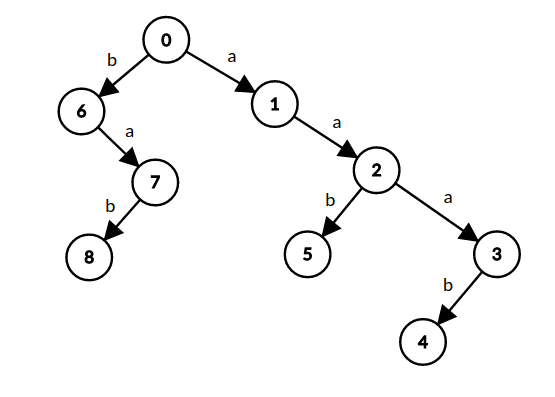
\includegraphics[width=0.4\textwidth]{graphics/trie-example.png}
    \caption{$\trie_{\{aaab, aab, bab, ba\}}$}
    \label{fig:trie}
\end{figure}

Zacznijmy temat konstrukcji od zdefiniowania funkcji, które będą nam potrzebne. Niech $\W$ oznacza zbiór wzorców, $\trie$ oznacza drzewo trie dla $\W$ (skrót dla $\trie_{\W}$), $\rot$ oznacza korzeń $\trie$, $\states$ oznacza zbiór wierzchołków $\trie$ (czyli docelowo zbiór stanów $\A$).

\begin{itemize}
    \item $\goto::\states\times\Sigma\mapsto\states$ -- ta funkcja w zasadzie reprezentuje zbiór krawędzi $\trie$; dodatkowo jednak, dla każdego symbolu w $\Sigma$, który nie etykietuje żadnej krawędzi wychodzącej z $\rot$, dodajemy pętlę w $\rot$; czyli:
    \begin{gather*}
        \goto(s_1, a)=\begin{cases}
        s_2 &\qquad \text{jeśli } (s_1,a,s_2)\in E[\trie] \\
        \rot &\qquad \text{jeśli } s_1=\rot\ \wedge\ \forall_{s}\ (\rot,a,s)\notin E[\trie] \\
        \none
        \end{cases}
    \end{gather*}

    \item $\out::\states\mapsto\wp(\W)$ -- jak zostało już wspomniane, chcemy w każdym stanie $s$ przechowywać listę wzorców, których wystąpienie w $T$ będzie poświadczone odwiedzeniem stanu $s$; w sporym zakresie możemy to obliczyć już przy konstrukcji $\trie$ (np. wracając do rysunku \ref{fig:trie}, $\out(1)=\emptyset$, $\out(5)=\{aab\}$, $\out(7)=\{ba\}$); będziemy musieli jeszcze jednak obsłużyć przypadki, gdy jeden wzorzec będzie sufiksem drugiego (np. $\out(4)=\{aaab, aab\}$)

    \item $\fail::\states\mapsto\states$ -- ostatecznie $\A$ będzie skonstruowane na wierzchołkach $\trie$ więc już teraz możemy spróbować zinterpretować obecność w stanie $s$ po przeczytaniu $j$-tego symbolu $T$ -- otóż etykiety na ścieżce pomiędzy $\rot$ a $s$ tworzą najdłuższy możliwy prefiks któregoś ze wzorców z $\W$, który da się dopasować w $T$ kończąc na pozycji $j$; funkcja $\goto$ jest częściowa, a więc dla niektórych stanów i niektórych symboli nie mamy zdefiniowanego przejścia (na razie otrzymamy $\none$); aby nie utknąć i zachować poprawność interpretacji, to $\fail(s)$ musi wskazywać na taki stan $s'$, żeby słowo powstałe ze ścieżki $\rot\rightsquigarrow s'$ było najdłuższym możliwym sufiksem słowa odpowiadającemu $\rot\rightsquigarrow s$; w dalszej części utożsamiać będziemy ścieżki ze słowami;

    Chodzenie krawędziami $\fail$ opiera się na identycznym pomyśle co rekurencyjne używanie tablic $Border$ w algorytmie Morrisa-Pratta. Warto również zauważyć, że $\fail$ nie ma sensu definiować dla $\rot$.

    \item $\cnext::\states\times\Sigma\mapsto\states$ -- trzy zdefiniowane funkcje powyżej zupełnie wystarczają, aby nasz docelowy automat robił to, czego pragniemy; jak jednak łatwo zauważyć, próba przeczytania jednego znaku z $T$ może wymagać więcej niż jednego przejścia krawędzią korzystając z $\goto$ oraz $\fail$ -- możemy musieć schodzić wzdłuż $\fail$ wielokrotnie; aby uniknąć tego, pod sam koniec utworzymy funkcję $\cnext$, która skompresuje nam tego typu ścieżki i zastąpi $\goto$ oraz $\fail$
\end{itemize}

\subsection{Obliczanie $\goto$, $\out$, $\fail$}
Jak już wiemy \textit{co} chcemy policzyć, to możemy przejść do tego \textit{jak} to zrobić. Funkcję $\goto$ oraz część $\out$, jak już zauważyliśmy, możemy obliczyć konstruując $\trie_{\W}$:
\begin{verbatim}
def _construct_goto(self, keywords, alphabet):
  for k, k_len in keywords:
    self._enter(k, k_len)

  for a in alphabet:
    if self._root.goto(a) is None:
      self._root.update_goto(a, self._root)

def _enter(self, keyword, keyword_len):
  current_state = self._root
  j = 1

  while j < keyword_len and current_state.goto(keyword[j]) is not None:
    current_state = current_state.goto(keyword[j])
    j += 1

  for a in keyword[j:keyword_len + 1]:
    next_state = AhoCorasickAutomaton.Node()
    current_state.update_goto(a, next_state)
    current_state = next_state

  current_state.append_outputs([(keyword, keyword_len)])
\end{verbatim}

Funkcja def \_enter(...) uzupełnia częściowo skonstruowane drzewo trie o ścieżkę dla podanego wzorca, w razie potrzeby tworząc nowe węzły. W pętli w wierszu 5. uzupełniamy definicję $\goto$ dla korzenia.

\vspace{10pt}

Funkcję $\fail$ powinniśmy obliczać dla coraz bardziej odległych od $\rot$ węzłów -- podobnie jak w algorytmie Morrisa-Pratta długości najdłuższych borderów obliczaliśmy na podstawie wartości dla krótszych słów:

\begin{verbatim}
def _construct_fail(self, alphabet):
  q = Queue()
  for s in (self._root.goto(a) for a in alphabet):
    if s != self._root:
      q.put(s)
      s.update_fail(self._root)

  while not q.empty():
    current = q.get()
    for a, child in ((a, current.goto(a)) for a in alphabet):
      if child is not None:
        q.put(child)

        fallback = current.fail()
        while fallback.goto(a) is None:
          fallback = fallback.fail()

        child_fallback = fallback.goto(a)
        child.update_fail(child_fallback)
        child.append_outputs(child_fallback.output())
\end{verbatim}

Przechodzimy zatem po $\trie$ za pomocą algorytmu BFS. Będąc w wierzchołku $\texttt{current}$, widząc krawędź etykietowaną przez $\texttt{a}$ do wierzchołka $\texttt{child}$, chcemy obliczyć $\fail(\texttt{child})$. Szukamy więc najdłuższego sufiksu słowa generowanego przez $\rot\rightsquigarrow\texttt{child}$ obecnego w $\trie$. Będzie to najdłuższy sufiks ścieżki $\rot\rightsquigarrow\texttt{current}$, który można przedłużyć o symbol $\texttt{a}$.

Znalazłszy odpowiedni wierzchołek $\texttt{child\textunderscore fallback}$ powiększamy zbiór $\out(\texttt{child})$ o wartości z  $\out(\texttt{child\textunderscore fallback})$ -- z indukcji wynika, że $\out(\texttt{child\textunderscore fallback})$ zawiera już wszystkie wzorce, które są sufiksami $\rot\rightsquigarrow\texttt{child\textunderscore fallback}$.

\subsection{Obliczanie $\cnext$}

Jeśli $\goto$ była określona dla $s\in\states$ oraz $a\in\Sigma$, to $\cnext(s, a) = \goto(s, a)$. W przeciwnym wypadku będąc w $s$ i chcąc przejść symbolem $a$, powinniśmy schodzić krawędziami $\fail$ tak długo, aż znajdziemy się w $s'$, dla którego $\goto(s', a)\neq\none$. Jest to podobny zabieg co poprawka Knutha do algorytmu Morrisa-Pratta.
\begin{verbatim}
def _construct_next(self, alphabet):
  q = Queue()
  for a in alphabet:
    a_child = self._root.goto(a)
    self._root.update_next(a, a_child)
    if a_child != self._root:
      q.put(a_child)
  self._root.use_only_next()

  while not q.empty():
    current = q.get()
    for a, child in ((a, current.goto(a)) for a in alphabet):
      if child is not None:
        q.put(child)
        current.update_next(a, child)
      else:
        fallback = current.fail()
        current.update_next(a, fallback.next(a))
    current.use_only_next()
\end{verbatim}

Instrukcje w wierszach 8. oraz 19. pozwalają zwolnić pamięć zapominając o wartościach funkcji $\goto$ i $\fail$. Formalnie dopiero teraz, struktura $\A$ ze zbiorem stanów $\states$ oraz funkcją przejścia $\cnext$ jest deterministycznym automatem skończonym.

\subsubsection{Analiza poprawności}
Z tego, co już zostało przedstawione, powinna wynikać poprawność zastosowanej metody. Aby jednak formalnie jej dowieść, wystarczy postawić trzy proste lematy:

\begin{lemma}{}{}
Niech $s,t\in\states$ i niech $u, v$ będą słowami generowanymi przez ścieżki $\rot\rightsquigarrow s$ i $\rot\rightsquigarrow t$. Wówczas $\fail(s) = t \iff v$ jest najdłuższym właściwym sufiksem $u$, który jest prefiksem pewnego $w_i\in\W$.
\end{lemma}

\begin{lemma}{}{}
Słowo $k$ należy do $\out(s)\iff$ $w\in\W$ oraz $k$ jest sufiksem słowa generowanego przez $\rot\rightsquigarrow s$.
\end{lemma}

\begin{lemma}{}{}
Po przeczytaniu $j$ znaków z $T$ znajdujemy się w stanie $s\iff$ słowo generowane przez $\rot\rightsquigarrow s$ jest najdłuższym sufiksem $T[1..j]$, który jest prefiksem pewnego $w\in\W$.
\end{lemma}

\noindent Ich uzasadnienia są prostymi dowodami rekurencyjnymi zapisanymi we fragmentach kodu powyżej.

\subsection{Analiza złożoności}
Konstrukcja całego automatu polega na sekwencyjnym wywołaniu procedur obliczających funkcje przejścia:

\begin{minted}[xleftmargin=20pt,linenos]{python}
class AhoCorasickAutomaton:
  def __init__(self, keywords, alphabet):
    self._root = AhoCorasickAutomaton.Node()
    self._construct_goto(keywords, alphabet)
    self._construct_fail(alphabet)
    self._construct_next(alphabet)
\end{minted}

Niech $m=\max_i |w_i|$. Bardzo łatwo zauważyć, że każdą z powyższych operacji wykonać można w czasie $\Otime(km)$ (dokładnie $\Theta(\sum_{i\in[k]}|w_i|)$) -- za każdym razem przechodzimy po całym drzewie $\trie$ odwiedzając każdy wierzchołek dokładnie raz oraz wykonując $\Theta(1)$ operacji w każdym z nich. Zakładamy również, że łączenie zbiorów $\out$ wykonuje się w czasie stałym (jak np. listy wiązane). Warto dodać, że moc $\Sigma$ wlicza się w zapotrzebowanie (zarówno pamięciowe jak i czasowe) liniowo -- rozmiar grafu jest z góry ograniczony przez $|\Sigma|\cdot km$ (z każdego wierzchołka może wychodzi $|\Sigma|$ krawędzi). Konstrukcja $\A$ oraz wyszukiwanie w $T$ odbywają się w czasie liniowo proporcjonalnym do wielkości $\trie$.

Pozostaje zastanowić się, ile czasu zajmie przeczytanie tekstu $T$ ($|T|=n$) i wypisanie wszystkich wystąpień wzorców. Moc $\Sigma$ traktujemy jak stałą.

Najpierw rozważmy sytuację, w której nie zgłaszamy żadnego wystąpienia wzorca (możemy np. tylko zaznaczyć pozycje $T$ o których wiemy, że na nich coś się kończy):
\begin{itemize}
    \item używając funkcji $\goto$ oraz $\fail$ wykonamy co najwyżej $2n$ przejść w $\A$ -- po przeczytaniu dowolnego symbolu przejdziemy dokładnie raz według funkcji $\goto$ i być może wielokrotnie krawędziami $\fail$; łatwo jednak zaobserwować, że każde przejście $\fail$ skraca odległość z obecnego wierzchołka do $\rot$, a z $\rot$ zawsze można wyjść używając $\goto$; zatem nie możemy przejść krawędziami $\fail$ więcej razy niż przeszliśmy $\goto$;

    można również spojrzeć na to w ten sposób, że przechodząc automatem $\A$ wzdłuż $T$, pamiętamy dwa wskaźniki w $T$ -- słowo pomiędzy nimi to właśnie to, które jest generowane przez ścieżkę z korzenia do obecnego wierzchołka; przejście $\goto$ przesuwa 'prawy' wskaźnik o 1 w prawo, przejście $\fail$ przesuwa 'lewy' wskaźnik o dodatnią liczbę pozycji w prawą, ale na tyle małą by nie przeskoczyć prawego;

    \item używając funkcji $\cnext$, przy każdym przeczytanym symbolu z $T$ wykonujemy zawsze jedno przejście -- $n$ ruchów
\end{itemize}

Problem może się pojawić, gdy będziemy chcieli wypisywać wszystkie wystąpienia wzorców. Pesymistycznym przykładem jest $\W=\{a,a^2,a^3,...,a^k\}$ oraz $T=a^n$. Liczba wystąpień będzie $\Theta(kn)$. Jednakże, nie jest to wada zastosowanego algorytmu -- każdy inny algorytm zgłaszający wszystkie wystąpienia wzorców musiałby wykonać co najmniej tyle samo pracy.

Zatem możemy określić złożoność czasową wyszukiwania wielu wzorców w tekście za pomocą automatu Aho-Corasick jako liniową w stosunku do sumy długości wszystkich wzorców oraz ilości ich wystąpień.

\subsubsection{Zastosowanie do wzorców 2D}
Okazuje się, że bardzo prosto można użyć automatu Aho-Corasick do wyszukiwania wzorców dwuwymiarowych. W skrócie:
\begin{enumerate}
    \item niech $T$ będzie kwadratową tablicą rozmiaru $n^2$, $P$ - kwadratową tablicą rozmiaru $m^2$ o różnych kolumnach, $m < n$
    \item niech $\W$ będzie zbiorem kolumn $P$
    \item automatem Aho-Corasick szukamy $\W$ w każdej z kolumn $T$; jeśli fragment $j$-tej kolumny od indeksu $i$ pokrywa się z $k$-tą kolumną $P$, to niech $T_P[i][j]=k$
    \item algorytmem KMP szukamy w każdym wierszu $T_P$ ciągu $(1,2,...,m)$
\end{enumerate}
Całość działa w czasie liniowym od wielkości wejścia i rozmiaru zbioru z którego pochodzą elementy w $T$ oraz $P$.


\subsection{Algorytm Commentz-Walter}
Algorytm Commentz-Walter to algorytm tekstowy służący do wyszukiwania wystąpień wzorca w tekście opracowany przez Beate Commentz-Walter (Uniwersytet Kraju Saary w Saarbrücken) w 1979 roku. Podobnie jak algorytm Aho-Corasick znajduje on w tekście wystąpienia słów ze słownika (pewnego zadanego zbioru wzorców), czyli jest w stanie jednocześnie w zadanym tekście wyszukiwać wiele wzorców. 

Algorytm Commentz-Walter jest merytorycznie ciekawy z tego powodu, że stanowi bardzo sprytną fuzję dwóch innych algorytmów, łącząc idee leżące u podstaw wspomnianego już algorytmu Aho-Corasick oraz algorytmu Boyera-Moore'a. Algorytm, o którym sobie dziś opowiemy, dla tekstu o długości $n$ i takiego zestawu wzorców, że najdłuższy spośród nich ma długość $m$, ma pesymistyczny czas działania $O(mn)$. W praktyce okazuje się jednak bardzo często, że czas działania tego algorytmu jest dużo lepszy. Stąd też nazwa pracy autorstwa Beate Commentz-Walter - ,,A String Matching Algorithm - Fast on the Average''. 

Najprawdopodobniej z powodu bardzo optymalnego średniego czasu działania, w GNU grep jest zaimplementowany algorytm wyszukujący wiele wzorców, bardzo podobny do oryginalnego algorytmu Commentz-Walter.

Najpierw przyjrzymy się nieco dokładniej dwóm głównym algorytmom, z których idei korzysta algorytm Commentz-Walter. Pierwszy z nich, algorytm Aho-Corasick jest jednym z algorytmów wyszukiwania wzorca w tekście. Znajduje on w tekście wystąpienia słów ze słownika (pewnego zadanego zbioru wzorców). Wszystkie wzorce są szukane jednocześnie, co powoduje, że złożoność obliczeniowa algorytmu jest liniowa od sumy długości wzorców, długości tekstu i liczby wystąpień wzorców w tekście. W tekście może jednak występować nawet kwadratowa od długości tekstu liczba wystąpień wzorców. 

Ideą algorytmu jest stworzenie drzewa trie o sufiksowych połączeniach pomiędzy wierzchołkami reprezentującymi różne słowa. Inaczej mówiąc tworzone jest drzewo (automat) o etykietowanych krawędziach, w którym każdy wierzchołek reprezentuje pewne słowo, składające się ze złączonych etykiet krawędzi znajdujących się na ścieżce od korzenia do tego węzła. Dodatkowo dołączane są krawędzie od wierzchołka do innego wierzchołka reprezentującego jego najdłuższy sufiks (fail). 

W czasie fazy wyszukiwania algorytm porusza się po tym drzewie zaczynając od korzenia i przechodząc do wierzchołka po krawędzi etykietowanej znakiem odczytanym z tekstu. W przypadku gdy takiej nie ma w drzewie, algorytm korzysta z krawędzi fail i tam próbuje przejść do wierzchołka po krawędzi etykietowanej odczytanym znakiem. W przypadku natrafienia na węzeł oznaczony jako koniec słowa, algorytm wypisuje je jako znalezione w tekście oraz sprawdza, czy czasem w tym miejscu nie kończy się więcej wzorców przechodząc krawędziami fail aż do korzenia sprawdzając, czy nie przechodzi po wierzchołku będącym końcem wzorca. 

Reasumując algorytm Aho-Corasick składa się z dwóch głównych faz, jedna to skonstruowanie odpowiedniego automatu dla zestawu podanych wzorców, a druga to użycie tego automatu do wyszukiwania tych wzorców w już podanym tekście. Oczywiście raz skonstruowany automat można wykorzystywać dowolnie wiele razy dla wielu różnych tekstów.

Drugi algorytm, z którego idei będziemy czerpać, to algorytm Boyera i Moore'a. Jest to algorytm wyszukiwania jednego wzorca w tekście. Polega na porównywaniu, zaczynając od ostatniego elementu wzorca. Jego główną zaletą jest to, że jeżeli okaże się, że znak, który aktualnie sprawdzamy, nie należy do wzorca, to możemy przeskoczyć w analizie tekstu o całą długość wzorca. Z reguły skoki wzorca są większe od $1$. Między innymi to sprawia, że algorytm ten jest często znacznie lepszy niż algorytm KMP, a także w przypadku, gdy algorytm Aho-Corasick jest uruchamiany z jednym wzorcem, to prawie na pewno algorytm Boyera-Moore'a poradzi sobie z nim szybciej niż algorytm Aho-Corasick. Asymptotycznie czas potrzebny na wyszukanie wszystkich wystąpień wzorca długości $m$, w tekście długości $n$ wynosi bardzo często średnio $O(n/m)$. Istnieją również ulepszenia oryginalnego algorytmu Booyera-Moore'a, które sprawiają, że faza wyszukiwania ma czas liniowy względem długości tekstu, nawet w przypadku pesymistycznym.

Uzbrojeni w to drobne przypomnienie dotyczące tych dwóch bazowych algorytmów jesteśmy gotowi przyjrzeć się algorytmowi Commentz-Walter. Algorytm ten podobnie jako Aho-Corasick składa się z dwóch faz. Pierwsza faza to zbudowanie struktury pozwalającej wyszukiwać wiele wzorców jednocześnie, a druga faza to już samo wyszukiwanie tych wzorców w konkretnym tekście. Wyszukiwanie zachowuje się dość podobnie jak wyszukiwanie w algorytmie Boyera-Moore'a, również osiągając średnio czas podliniowy względem rozmiaru tekstu. W kolejnych sekcjach tego omówienia przyjrzymy się z detalami kolejnym fazom tego algorytmu, a na koniec skomentujemy szerzej czas jego działania.

Do przechowywania w pamięci pewnego zestawu wzorców w użyteczny sposób pomocna będzie nam następująca struktura:

\begin{definition}{}{}
\textbf{Drzewem trie} nazywamy takie ukorzenione drzewo $T$, że:
\begin{enumerate}
    \item Każdy wierzchołek $v \in T$, poza korzeniem $r$ ma pewną etykietę $a = l(v)$. Jest to element ustalonego alfabetu $\Sigma$.
    \item Korzeń $r$ ma przypisaną etykietę $\epsilon$, za pomocą której oznaczamy puste słowo.
    \item Jeżeli wierzchołki $v_1$, $v_2$ są różnymi dziećmi tego samego wierzchołka $v$, to $l(v_1) \neq l(v_2)$.
\end{enumerate}
\end{definition}

\noindent Mówimy, że ścieżka $v_1, \cdots, v_k$ (gdzie $v_{i+1}$ jest synem $v_i$) w drzewie trie $T$ \textbf{reprezentuje} słowo $l(v_1)\cdots l(v_k)$. Słowo to oznaczamy za pomocą $w(v_k)$, jeżeli $v_1 = r$. Dodatkowo 

\begin{definition}{}{}
dla każdego węzła $v\in T$ definiujemy jego \textbf{głębokość} $d(v) := 0$, jeżeli $v=r$ oraz $d(v) := d(v') + 1$, jeżeli wierzchołek $v$ jest synem $v'$.
Dodatkowo wprowadzamy oznaczenie na \textbf{głębokość całego drzewa trie} $d(T) := \max \{ d(v) : v \in T\}$.
\end{definition}

Niech $\mathcal{W} = \{ w_1, \cdots, w_r\}$ będzie zbiorem wzorców nad pewnym alfabetem $\Sigma$, które będziemy chcieli wyszukiwać w pewnym tekście $t$. Podobnie jak w algorytmie Aho-Corasick reprezentujemy zbiór $\mathcal{W}$ za pomocą drzewa trie $T$. \textbf{Główna różnica polega na tym, że nie trzymamy w drzewie trie wzorców, ale odwrócone wzorce.} Dokładniej dla każdego $h = 1,\cdots, r$ istnieje wierzchołek $v_h \in T$ reprezentujący odwrócony wzorzec $w_h^R$. Dodatkowo każdy wierzchołek drzewa trie jest wyposażony w tak zwaną \textbf{funkcję wyjścia} zdefiniowaną jako $out(v) := \{ w : w^R = w(v)\}$. 

Główna idea tego algorytmu zawiera się w dodaniu do drzewa trie dwóch funkcji \textbf{shift1} i \textbf{shift2}. Są to funkcje, które przypisują wierzchołkom drzewa trie liczby naturalne, które to liczby będą nam bardzo pomocne w fazie wyszukiwania, aby symulować przesunięcia znane z algorytmu Boyera-Moore'a. Formalna definicja tych funkcji jest następująca i wykorzystuje definicje dwóch typów zbiorów. Mianowicie 

\begin{definition}{}{}
dla każdego $v \not = r, v \in T$, definiujemy
zbiór $set1(v)$ jako zbiór tych wszystkich wierzchołków $v'$, że $w(v)$ jest poprawnym sufiksem słowa $w(v')$, tzn. $w(v') = uw(v)$, dla pewnego niepustego słowa $u$. Definiujemy również zbiór $set2(v)$ jako zbiór tych wszystkich wierzchołków $v'$ takich, że $v' \in set1(v)$ oraz $out(v') \not = \emptyset$. 
\end{definition}

\noindent Przydadzą nam się jeszcze oznaczenia $wmax := \max_{1 \leq h \leq r}|w_h|$ oraz $wmin := \min_{1 \leq h \leq r}|w_h|$. Teraz jesteśmy już gotowi zdefiniować funkcje przesunięcia i definicje te są następujące.

\begin{definition}{}{}
dla każdego $v \in T$ definiujemy funkcję \textbf{shift1} jako $shift1(v) := 1$ jeżeli $v=r$. W przeciwnym przypadku $$shift1(v) :=  min \left( \{d(v')-d(v) : v' \in set1(v) \} \cup \{wmin\}\right)$$
\end{definition}

\begin{definition}{}{}
dla każdego $v \in T$ definiujemy funkcję \textbf{shift2} jako $shift2(v) := wmin$ jeżeli $v=r$. W przeciwnym przypadku $$shift2(v) :=  min \left( \{d(v')-d(v) : v' \in set2(v) \} \cup shift2(parent(v))\right)$$
\end{definition}

\noindent Ostatnia funkcja, którą będziemy potrzebować to funkcja $char: \Sigma \longrightarrow \mathrm{N}$ zdefiniowana jako $$char(a) := \min (\{ d(v) : l(v) = a \} \cup \{ wmin+1 \})$$

\noindent Poniżej mamy przykład (pochodzący z oryginalnej pracy) tak zbudowanej struktury dla zbioru wzorców $\{cacbaa, acb, aba, acbab, ccbab\}$, gdzie $wmin = 3$. Na poniższej ilustracji dla każdego wierzchołka $v \not = r$, ostrzałkowane linie ciągłe wskazują na elementy zbioru $set2(v)$, natomiast ostrzałkowane, jak i przerywane linie wskazują na elementy zbioru $set1(v)$.

\begin{center}
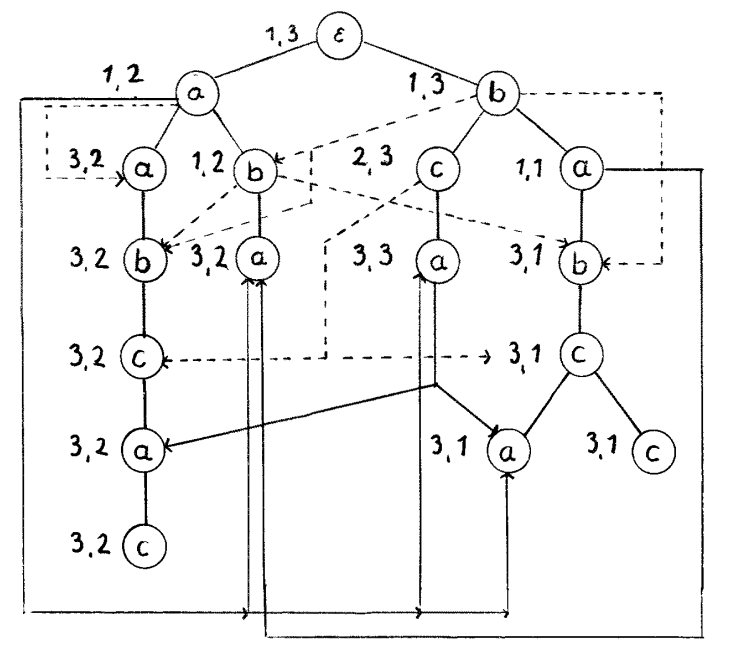
\includegraphics[scale=0.4]{graphics/trie-example-2.png}
\end{center}

\subsubsection{Faza wyszukiwania w tekście}
Wynikiem tej fazy jest lista par postaci $(w, i)$, gdzie $w$ to któryś z szukanym wzorców, natomiast $i$ to pozycja w tekście, na której został znaleziony wzorzec $w$. Faza ta działa następująco. Załóżmy, że mamy już zbudowane drzewo trie składające się z wszystkich wzorców, ale wstawionych do drzewa trie w odwróconej kolejności. Cała sztuczka polega teraz na tym, że dopasowywanie robimy jak w algorytmie Aho-Corasick chodząc po drzewie trie, ale korzystając z pomysłu zapożyczonego z algorytmu Boyera-Moore'a, w przypadku niezgodności znaków używamy funkcji shift1 oraz shift2, aby wykonać odpowiedni skok w tekście, w którym dopasowujemy wzorce z drzewa trie. Zamieszczony poniżej pseudokod dość dokładnie tłumaczy jak wygląda ta kluczowa faza algorytmu.

\begin{algorithm}
\caption{Commentz-Walter, faza wyszukiwania}\label{euclid}
\begin{algorithmic}
\Procedure{Commentz-Walter-search}{$text, n, trie$} \Comment{tekst, długość, drzewo trie wzorców}
\State $v := root(r)$ \Comment{obecnie przetwarzany wierzchołek trie}
\State $i := wmin$ \Comment{obecnie przetwarzana pozycja w tekście}
\State $j := 0$ \Comment{głębokość $v$ w drzewie trie}

\State While{ $j \leq n$ }
    \State While {$\exists$ dziecko $v'$ wierzchołka $v$ takie, że $l(v')=t[i-j]$} \Comment{faza skanowania}
        \State $v = v'$
        \State $j = j + 1$
        \State \textbf{yield} $(w, i)$ dla każdego $w \in out(v)$
    \State EndWhile
\State $shift(v, t[i-j]) := \min(\max(shift1(v), char(t[i-j])-j-1), shift2(v))$
\State $i = i + shift(v, t[i-j])$ \Comment{faza przesuwania tekstu}
\State $j = 0$
\State EndWhile
\EndProcedure
\end{algorithmic}
\end{algorithm}

Pozostaje uzasadnić, że ten algorytm na pewno zwraca wszystkie wystąpienia wzorców w tekście. Nie ma wątpliwości co do tego, że każda zwrócona para $(w, i)$ jest na pewno dobrym wystąpieniem. Pozostaje więc się upewnić, że na pewno żadne wystąpienie któregoś z wzorców nie jest pomijane. Z budowy algorytmu wynika, że jedynym podejrzanym miejscem jest moment robienia przesunięcia w tekście. Potrzebujemy, więc podać argument, że $t[i-j+1]\cdots t[i] = w_t^R(v)$ dla pewnego $v \in T$ implikuje, że nie istnieje takie $i'$, że $i < i' < s(v, t[i-j])$ oraz $t[i'-|w|+1]\cdots t[i']$ dla pewnego wzorca $w$. Jednak z definicji $s(v, t[i-j])$ mamy tę własność po prostu za darmo.

\subsubsection{Faza przygotowania wzorców}
W tej fazie algorytmu na wejściu mamy zbiór wzorców, a na wyjściu chcemy mieć drzewo trie dla tego zestawu wzorców oraz obliczone dla niego funkcje out, shift1, shift2 oraz char. Chcielibyśmy to wszystko zrobić w czasie liniowym względem sumy długości wzorców. Oczywiście konstrukcja trie w takim czasie jest natychmiastowo. Po prostu dodajemy kolejne słowa budując jednocześnie drzewo. Z definicji funkcji char i out również wynika prostota ich obliczania wprost z definicji. Kłopotliwe mogą się wydawać na pierwszy rzut oka kluczowe funkcje shift1 oraz shift2.

Jednak cały problem mamy już rozwiązany za pomocą algorytmu Aho-Corasick. Mianowicie rozważmy pewną funkcje $f$ zdefiniowaną na wierzchołkach drzewa trie $T$ za pomocą formuły $f(v') = v$, jeżeli $w(v)$ jest maksymalnym sufiksem właściwym $w(v')$ w drzewie $T$. Funkcja ta idealnie współgra z funkcją fail z automatu Aho-Corasick, więc to co musimy zrobić, aby ją obliczyć, to odpalić fazę konstrukcji z algorytmu Aho-Corasick i w czasie jednego przejścia algorytmem bfs po drzewie trie obliczyć funkcję fail. Okazuje się bowiem, że funkcja $set1'$ odwrotna do funkcji $f$, czyli $set1'(v) = \{v' : f(v')=v \}$, to dokładnie podzbiór szukanego przez nas zbioru $set1$, który potrzebujemy do obliczenia funkcji przesunięć. Ponadto zawiera on wierzchołki $v' \in set1(v)$ takie, że $d(v')-d(v)$ jest minimalne. Wynika stąd, że funkcję shift1 można istotnie obliczyć w czasie liniowym. Analogicznie obliczamy funkcję shift2 rozważając zbiór $set2'(v) = \{ v' : v' \in set1'(v), out(v') \not = \emptyset\}$. 

\subsection{Złożoność obliczeniowa algorytmu}
Faza konstrukcji drzewa trie opisana powyżej jest wykonywana w czasie liniowym względem sumy długości wszystkich wzorców. Przeszukiwanie tekstu pesymistycznie może mieć czas liniowy względem iloczynu długości tekstu, w którym wyszukujemy, z długością najdłuższego wzorca, ale dzięki temu, że mamy funkcje przesunięć, bardzo często nie skanujemy całego tekstu znak po znaku, tylko jego części. Poprzez silną analogię do algorytmu Boyera-Moore'a stwierdzamy, że algorytm Commentz-Walter, działa średnio podobnie jak algorytm Boyera-Moore'a, czyli bardzo szybko. Pesymistycznie jednak pamiętać należy, że może mieć złożoność $O(nm)$, gdzie $n$, to długość tekstu, a $m$ to długość najdłuższego wzorca.

\nocite{*}
\printbibliography

\end{document}
